\documentclass[a4paper]{tmanotes}


% Paths
\newcommand{\figs}{../figs}
\newcommand{\data}{../data}

% Fonts
\usepackage{newpxtext,newpxmath}
\renewcommand*\sfdefault{cmss}

% Double hlines
\usepackage{hhline}

% Listings
\usepackage{textcomp}
\usepackage{listings}
\lstset{
  keywordstyle=\bfseries\color{orange},
  stringstyle=\color{darkblue!80},
  commentstyle=\color{darkblue!80},
  showstringspaces=false,
  basicstyle=\ttfamily,
  upquote=true,
}
\lstdefinestyle{fortran}{
  language=Fortran,
  morekeywords={for},
  deletekeywords={status},
}
\lstdefinestyle{c}{
  language=C,
  morekeywords={include},
}
\lstdefinestyle{shell}{
  language=bash,
}


\newtheorem{ex}{Exercise}[chapter]


% Tikz
\usepackage{tikz}
\usetikzlibrary{positioning,shapes,arrows,calc,intersections}


% Make footnotes work inside tables
\usepackage{footnote}
\makesavenoteenv{tabular}
\makesavenoteenv{table}

% Numbering
\makeatletter
\AtBeginDocument{%
  \let\c@lstlisting\c@figure
  \let\c@table\c@figure
}
\makeatother


% Units
\usepackage[detect-weight=true, binary-units=true]{siunitx}
\DeclareSIUnit\flop{Flops}

%-------------------------------------------------------------------------------
% @collection	Discretization
% @description
% @version		1
% @author		Aurélien Larcher <aurelien.larcher@gmail.com>
%-------------------------------------------------------------------------------
% @category		Discretization
%---------------------------------------
% @subcategory	Discretization subscript
% @macro disc		admissible discretization
\newcommand{\disc}{{\mathcal M}}
% @macro disc		space-time discretization
\newcommand{\discd}{{\mathcal D}}
% @macro disc		simplicial discretization
\newcommand{\disct}{{\mathcal T}}
%---------------------------------------
% @subcategory	Mesh
% @macro mesh		admissible finite volume mesh
\newcommand{\mesh}{{\mathcal M}}
% @macro xD
\newcommand{\xD}{{\rm D}}
% @macro size		size
\newcommand{\size}{{\rm size}}
%---------------------------------------
% @subcategory	Mesh topology
\newcommand{\mgraph}[2]{\bigl(\;#1,\:#2\;\bigr}
% @macro connect		connectivity
\newcommand{\connect}[2]{{\mathcal C}_{#1, #2}}
% @macro edges		set of cells of the discretization
\newcommand{\cells}{{\mathcal{K}}}
\newcommand{\cell}{{K}}
% @macro edges		set of vertices of the discretization
\newcommand{\vertices}{{\mathcal{V}}}
\newcommand{\vertex}{{\mathrm v}}
%---------------------------------------
% @subcategory	Edges
% @macro edge		edge
\newcommand{\edge}{\sigma}
% @macro edged		edge of diamond cell
\newcommand{\edged}{\xi}
% @macro edges		set of edges of the discretization
\newcommand{\edges}{\mathcal{E}}
% @macro edgesint	set of internal edges
\newcommand{\edgesint}{\edges_{{\rm int}}}
% @macro edgesext	set of external edges
\newcommand{\edgesext}{\edges_{{\rm ext}}}
% @macro edgesextD	set of external edges of the diamond mesh
\newcommand{\edgesextD}{{\cal E}_{{\rm ext,D}}}
% @macro nK			outward normal from K across edge
\newcommand{\nK}{\bfn_{\edge,K}}
% @macro nL			outward normal from L across edge
\newcommand{\nL}{\bfn_{\edge,L}}
% @macro nedge		normal vector on edge
\newcommand{\nedge}{\bfn_\edge}
% @macro nKL 		outward normal from K to L
\newcommand{\nKL}{\bfn_{KL}}

% @macro 			points	set of points of the discretization
\newcommand{\points}{\mathcal{P}}
% @macro neigh		neighbouring cells of K
\newcommand{\neigh}{{\mathcal N}(K)}

%-------------------------------------------------------------------------------
% @collection	Finite Element Method
% @description
% @version		1
% @author		Aurélien Larcher <aurelien.larcher@gmail.com>
%-------------------------------------------------------------------------------

\newcommand{\uh}{{u_h}}
\newcommand{\vh}{{v_h}}
\newcommand{\uuh}{{\boldsymbol u}_h}
\newcommand{\vvh}{{\boldsymbol v}_h}
\newcommand{\meshT}{{\mathcal T}_h}
\newcommand{\sizeT}{h_{\mathcal T}}
\newcommand{\CellK}{{K}}
\newcommand{\SpaceP}{{\mathcal P}}
\newcommand{\DualBasis}{{\Sigma}}
\newcommand{\RefK}{{\hat \CellK}}
\newcommand{\RefP}{{\hat \SpaceP}}
\newcommand{\RefSigma}{{\hat\DualBasis}}
\newcommand{\FE}{{(\CellK,\SpaceP, \DualBasis)}}
\newcommand{\RefFE}{{(\RefK,\RefP, \RefSigma)}}
\newcommand{\Ndof}{{N_{\mathrm dof}}}
\newcommand{\NxVh}{{N_{\xVh}}}
\newcommand{\Res}[1]{{\mathcal{R}(#1)}}
\newcommand{\ResK}[1]{{\mathcal{R}_K(#1)}}
\newcommand{\Stab}{\mathcal{S}}
\newcommand{\Etol}{\epsilon_{\mathrm tol}}
\newcommand{\EindK}{\epsilon_K}
\newcommand{\EindT}{\epsilon_{\mathcal T}}

\newcommand{\Iop}[1]{\mathop{\mathcal{I}_{#1}}}
\newcommand{\IopK}[1]{\mathop{\mathcal{I}_{K,#1}}}

% @category		Discrete spaces
%---------------------------------------
\newcommand{\xM}{{M}}
\newcommand{\xMh}{{\xM}_h}
\newcommand{\xMker}{{\xM}_0}
\newcommand{\xMz}{{\mathrm{\tilde M}}}
\newcommand{\xMzh}{{\mathrm{\tilde M}_h}}
\newcommand{\xV}{{V}}
\newcommand{\xVh}{{\xV}_h}
\newcommand{\xVdisc}{{\xV}_h}
\newcommand{\xVdiscm}{{\xVdisc}^{(m)}}
\newcommand{\xVd}{\boldsymbol{\xV}}
\newcommand{\xVhd}{\boldsymbol{\xV}_h}
\newcommand{\xVV}{\boldsymbol{W}}
\newcommand{\xWd}{\boldsymbol{\xVV}}
\newcommand{\xWdisc}{{\boldsymbol W}_h}
\newcommand{\xWdiscm}{{\xWdisc}^{(m)}}
\newcommand{\xPzero}{{\xP}_1}
\newcommand{\xPone}{{\xP}_1}
\newcommand{\xPtwo}{{\xP}_2}
\newcommand{\xPn}[1]{{\xP}_{#1}}
\newcommand{\xQone}{{\xQ}_1}
\newcommand{\xisoQone}{\tilde {\xQ}_1}
\newcommand{\xQtwo}{{\xQ}_2}
%-------------------------------------------------------------------------------
% @category		Operators
\newcommand{\Ph}{{\Pi_h}}
\newcommand{\rh}{{r_h}}
\newcommand{\rhv}{\boldsymbol{r}_h}
\newcommand{\Gradh}{{\boldsymbol \nabla_h}}
\newcommand{\Divh}{{\boldsymbol \nabla_h\cdot}}
\newcommand{\Divrh}{{\mathop{\mathrm div}_h}}
\newcommand{\Stabh}[1]{{S_h^{#1}}}
%-------------------------------------------------------------------------------
\def\snormFE{\norm}
\newcommand{\refelm}{\hat K}

%-------------------------------------------------------------------------------
% @collection	Latin Locutions
% @description 
% @version		1
% @author		Aurélien Larcher <aurelien.larcher@gmail.com>
%-------------------------------------------------------------------------------
\newcommand{\apriori}{\textit{a priori\/} }
\newcommand{\afortiori}{\textit{a fortiori\/} }
\newcommand{\aposteriori}{\textit{a posteriori\/} }
\newcommand{\cf}{\textit{cf.\/} }
\newcommand{\eg}{\textit{e.g.\/} }
\newcommand{\etal}{\textit{et al.\/} }
\newcommand{\etc}{\textit{etc\/} }
\newcommand{\ie}{\textit{i.e.\/} }
\newcommand{\loccit}{\textit{a loc. cit.\/} }
\newcommand{\vg}{\textit{v.g.\/} }

%-------------------------------------------------------------------------------
% Operators:
%-------------------------------------------------------------------------------
\newcommand{\Lgr}[2]{\mathcal L^{#1}_{#2}}
\newcommand{\Abs}[1]{\left\lvert #1 \right\rvert}
\newcommand{\card}{\mathrm{card}}
\newcommand{\fromto}{\rightarrow}
\newcommand{\tendsto}{\rightarrow}
\newcommand{\tendstoweak}{\rightharpoonup}
\newcommand{\forany}{{\forall\;}}
\newcommand{\m}{{(m)}}
\newcommand{\seq}[1]{\bigl({#1}^\m\bigr)_{m\in\xN}}
\newcommand{\seqn}[1]{\left({#1}^n\right)_{n\in\xN}}
\newcommand{\Proj}[1]{\,\mathrm{P}_{#1}\,}
\newcommand{\Projh}[1]{\,\mathrm{\pi}_{#1}\,}
\newcommand{\opA}{\mathcal{A}}

\newcommand{\Empty}{\varnothing}
\newcommand{\Union}{\mathop\bigcup}
\newcommand{\Inter}{\mathop\bigcap}
\newcommand{\Interior}[1]{\mathring{#1}}



%-------------------------------------------------------------------------------
% Miscellaneous
\newcommand{\Grp}[1]{\displaystyle\left({#1}\right)}
\newcommand{\indic}[1]{\displaystyle{1\!\!1_{#1}}}
\newcommand{\mean}[1]{\brace\lbrace#1\rbrace\rbrace}
\newcommand{\jump}[1]{[#1]}
% @macro diam		diameter
\newcommand{\diam}{{\mathrm diam}}

%-------------------------------------------------------------------------------
% Derivatives
\newcommand{\ds}{\hspace{.5ex}{\mathrm d}s}
\newcommand{\md}{\hspace{.5ex}{\mathrm d}}
%
\newcommand{\dt}{\delta \hspace{-0.05ex} t}
\newcommand{\pdt}{\partial_t}
\newcommand{\ddt}{\hspace{.5ex}{\mathrm d}t}
%
\newcommand{\pd}[1]{\partial_{#1}\,}
\newcommand{\pdx}{\partial_x}
\newcommand{\dxd}{\hspace{.5ex}{\mathrm d}\bfx}
\newcommand{\dx}{\hspace{.5ex}{\mathrm d}\bfx}
\newcommand{\dy}{\hspace{.5ex}{\mathrm d}\bfy}
\newcommand{\dz}{\hspace{.5ex}{\mathrm d}\bfz}
%\newcommand{\ddx}{\frac{{\mathrm d}}{{\mathrm d}x}}
%\newcommand{\ddy}{\frac{{\mathrm d}}{{\mathrm d}y}}
%\newcommand{\ddz}{\frac{{\mathrm d}}{{\mathrm d}z}}
\newcommand{\ddx}{\frac{{\partial}}{{\partial}x}}
\newcommand{\ddy}{\frac{{\partial}}{{\partial}y}}
\newcommand{\ddz}{\frac{{\partial}}{{\partial}z}}

\newcommand{\pddx}[1]{\frac{{\partial #1}}{{\partial}x}}
\newcommand{\pddy}[1]{\frac{{\partial #1}}{{\partial}y}}
\newcommand{\pddz}[1]{\frac{{\partial #1}}{{\partial}z}}
\newcommand{\dd}[2]{\frac{{\partial #1}}{{\partial#2}}}
\newcommand{\ddd}[1]{\frac{{\mathrm d}}{{\mathrm d #1}}}

%-------------------------------------------------------------------------------
\newcommand{\xDot}{\,{\mathbf\cdot}\,}
\newcommand{\Cross}{\mathbf X}
\newcommand{\DualP}[2]{\mathbf{\langle}\;#1\:,\: #2 \;\mathbf{\rangle}}
\newcommand{\Inner}[2]{{{\scriptstyle\mathbf{(}}\;#1\:,\: #2 \;{\scriptstyle\mathbf{)}}}}
\newcommand{\InnerP}[3]{{{\scriptstyle\mathbf{(}}\;#1\:,\: #2 \;{\scriptstyle\mathbf{)}}}_{\,#3}}
\newcommand{\Span}{\mathop{\mathrm{span}}}
\newcommand{\T}{{^{\mathrm T}}}
\newcommand{\Trace}[2]{{\mathbf{Tr}}^{(#1)}(#2)}
\newcommand{\trans}{{^{\mathsmaller{T}}}}
\newcommand{\Tens}{{\otimes}}
\newcommand{\Vect}{\wedge}

%-------------------------------------------------------------------------------
% Differential Operators
% continuous
\newcommand{\D}{{\boldsymbol{\mathrm D}}} % gradient
\newcommand{\Grad}{{\boldsymbol\nabla}} % gradient
\newcommand{\Gradt}{{\boldsymbol\nabla^t}}
\newcommand{\Gradx}{\Grad_x}
\newcommand{\GradxR}{\Grad_{\xR}}
\newcommand{\Div}{{\boldsymbol\nabla\cdot\,}} % divergence
\newcommand{\Divr}{{\mathrm div}}
\newcommand{\Lap}{{\boldsymbol\Delta}} % laplacian
\newcommand{\Lapl}{{\boldsymbol\nabla^2}} % laplacian
\newcommand{\Curl}{{\Grad\boldsymbol\wedge}}
%
\newcommand{\udiv}{(\vec{\bfv}\cdot\nabla)} % advection
\newcommand{\uhdiv}{(\vec{\bfv_h}^n\cdot\nabla)}

\newcommand{\DualProd}[2]{{\langle #1,\: #2 \rangle}}

%-----------------------------------------------------------------------
%   Thermophysical Properties
%-----------------------------------------------------------------------
\newcommand{\dens}{\varrho}             % density
\newcommand{\cond}{\lambda}             % conductivity
\newcommand{\visc}{\eta}                % dynamic viscosity ($Pa.s$)
\newcommand{\kvisc}{\nu}                % kinematic viscosity ($m^2/s$)
\newcommand{\tension}{\sigma}           % surface tension
\newcommand{\Tt}{\Sigma}                % surface tension
\newcommand{\Ttm}{\underline{\Sigma}}   % constante
\newcommand{\cp}{c_p}                   % chaleur massique
\newcommand{\grav}{\mathbf g}           % gravity
\newcommand{\fric}{\xi}                 % coefficient de friction
\newcommand{\Stress}{\sigma}    % stress tensor
\newcommand{\Tvisc}{\tau}       % viscous stress tensor
\newcommand{\Strain}{\varepsilon}    % strain tensor

%-----------------------------------------------------------------------
%   Non dimensional numbers
%-----------------------------------------------------------------------
\newcommand{\CFL}{{\rm CFL}}            % CFL number
\newcommand{\Fr}{{\rm\bf Fr}}           % Froude number
\newcommand{\Nu}{{\rm\bf Nu}}		% Nusselt
\newcommand{\Pra}{{\rm\bf Pr}}		% Prandtl
\newcommand{\Rey}{{\rm\bf Re}}		% Reynodls
\newcommand{\We}{{\rm\bf We}}		%
\newcommand{\Ca}{{\rm\bf Ca}}		%
\newcommand{\La}{{\rm\bf La}}		%
\newcommand{\Ra}{{\rm\bf Ra}}		% Rayleigh
\newcommand{\Eo}{{\rm\bf Eo}}		%
%\newcommand{\Eot}{E\"otv\"os }		
\newcommand{\Pe}{{\rm\bf Pe}}		% Peclet
\newcommand{\Mor}{{\rm \bf M}}
\newcommand{\Adim}[1]{#1_{\diamond}}
\newcommand{\Ref}[1]{{#1}_{\rm ref}}    % deference quantity for adim


%-------------------------------------------------------------------------------
% @collection	Spaces (M2AN style)
% @description
% @version		1
% @author		Aurélien Larcher <aurelien.larcher@gmail.com>
%-------------------------------------------------------------------------------
% @category		Sets
%---------------------------------------

\newcommand{\aevery}{\textit{a.e\/} }

\newcommand{\dual}{^\star}
\newcommand{\ortho}{^\perp}
\newcommand{\ball}{\mathfrak B}

\newcommand{\cyl}{\mathrm{Q}} % Q = \dom \times (0,T)
\newcommand{\dom}{\Omega}
\newcommand{\domc}{\overline{\Omega}}
\newcommand{\bound}{{\partial\dom}}

% Integral on the space domain
\newcommand{\intD}{\int_\dom}
% Integral on the time interval
\newcommand{\intI}{\int_0^T}

%-------------------------------------------------------------------------------

\newcommand{\kernel}{\mathfrak N}
\newcommand{\nilset}{\lbrace 0\rbrace}
\newcommand{\range}{\mathfrak R}
\newcommand{\Fam}[1]{{\left\lbrace #1 \right\rbrace}}
\newcommand{\sFam}[1]{{\lbrace #1 \rbrace}}
\newcommand{\Set}[1]{{\left\lbrace #1 \right\rbrace}}
\newcommand{\One}{{\displaystyle{1\!\!1}}}
\newcommand{\xLin}{\mathcal{L}}
\newcommand{\Ker}{\mathrm{Ker}}
\newcommand{\Ima}{\mathrm{Im}}
\newcommand{\Basis}{\mathcal{B}}
\newcommand{\Coords}[1]{\left(#1\right)}

\newcommand{\cyldisc}{\mathrm{Q}_\discd}
\newcommand{\intdisc}[1]{[\hspace{-.02in}[{ #1}]\hspace{-.02in}]}

%-------------------------------------------------------------------------------

\newcommand{\xK}{\mathbb{K}}
\newcommand{\xR}{\mathbb{R}} %M2AN
\newcommand{\xQ}{\mathbb{Q}} %M2AN
\newcommand{\xZ}{\mathbb{Z}} %M2AN
\newcommand{\xN}{\mathbb{N}} %M2AN
\newcommand{\xP}{\mathbb{P}} %M2AN
\newcommand{\xA}{\mathbb{A}} %M2AN
\newcommand{\xComplex}{\mathbb{C}}
\newcommand{\xQuaternion}{\mathbb{H}} %M2AN
\newcommand{\xHil}{H}

% d-dimensional versions
\newcommand{\xKd}{{\xK^d}}
\newcommand{\xRd}{{\xR^d}}
\newcommand{\xQd}{{\xQ^d}}
\newcommand{\xZd}{{\xZ^d}}
\newcommand{\xNd}{{\xN^d}}
\newcommand{\xPd}{{\xP^d}}
\newcommand{\xAd}{{\xA^d}}

\newcommand{\xRn}{{\xR^n}}
\newcommand{\xRN}{{\xR^N}}

%-------------------------------------------------------------------------------
% @category		Space of Matrices
\newcommand{\xMat}{\mathcal{M}}
\newcommand{\xMatR}[1]{\mathcal{M}_{#1}(\xR)}
\newcommand{\xMnR}{{M_n(\xR)}}
\newcommand{\xMNR}{{M_N(\xR)}}
\newcommand{\xGL}{\mathop{\mathrm GL\,}\nolimits}
\newcommand{\xGLnR}{{\mathop{\mathrm GL_n(\xR)\,}\nolimits}}
\newcommand{\xGLNR}{{\mathop{\mathrm GL_N(\xR)\,}\nolimits}}
\newcommand{\xSL}{\mathop{\mathrm SL\,}\nolimits}
\newcommand{\xPSL}{\mathop{\mathrm PSL\,}\nolimits}
\newcommand{\xSO}{\mathop{\mathrm SO\,}\nolimits}
\newcommand{\xSU}{\mathop{\mathrm SU\,}\nolimits}

%-------------------------------------------------------------------------------
% @category		Continuously Differentiable Functions
\newcommand{\xC}{{\mathrm C}} %M2AN
\newcommand{\xCzero}{\xC^{0}} %M2AN
\newcommand{\xCone}{\xC^{1}} %M2AN
\newcommand{\xCtwo}{\xC^{2}} %M2AN
\newcommand{\xCinfty}{\xC^{\infty}} %M2AN
\newcommand{\xCn}[1]{\xC^{#1}} %M2AN
\newcommand{\xCinfc}{{\xCinfty_c}}

%-------------------------------------------------------------------------------
% @category		Lebesgue Spaces
\newcommand{\xL}{{\mathrm L}}
\newcommand{\xLzero}{\xL^{0}}
\newcommand{\xLone}{\xL^{1}}
\newcommand{\xLoneloc}{\xLone_{loc}}
\newcommand{\nLone}[1]{\norm{#1}_{\xLone(\dom)}}
\newcommand{\nLoned}[1]{\norm{#1}_{\xLone(\dom)^d}}
\newcommand{\xLtwo}{\xL^{2}}
\newcommand{\nLtwo}[1]{\norm{#1}_{\xLtwo(\dom)}}
\newcommand{\nLtwod}[1]{\norm{#1}_{\xLtwo(\dom)^d}}
\newcommand{\xLtwoR}[1]{{\xLtwo(#1)/\xR}}
\newcommand{\xLtwoz}{\xLtwo_0}
\newcommand{\xLp}[1]{\xL^{#1}}
\newcommand{\nLp}[2]{\norm{#2}_{\xLp{#1}(\dom)}}
\newcommand{\xLinfty}{\xL^{\infty}}
\newcommand{\nLinfty}[1]{\norm{#1}_{\infty}}

%-------------------------------------------------------------------------------
% @category		Hardy Spaces
\newcommand{\xH}{{\mathrm H}} %M2AN
\newcommand{\xHd}{\boldsymbol{\mathrm H}}
\newcommand{\xHzero}{\xH^{0}} %M2AN
\newcommand{\xHone}{\xH^{1}} %M2AN
\newcommand{\xHoned}[1]{{\xHone(#1)^d}}
\newcommand{\xHonec}{{\xHone_0}}
\newcommand{\xHonecb}{{\xHone_{0,b}}}
\newcommand{\xHonecd}[1]{{\xHonec(#1)^d}}
\newcommand{\xHtwo}{\xH^{2}} %M2AN
\newcommand{\xHinfty}{\xH^{\infty}} %M2AN
\newcommand{\xHn}[1]{\xH^{#1}} %M2AN
\newcommand{\xHmone}{\xH^{-1}}
\newcommand{\xHmoned}[1]{{\bigl(\xHmone(#1)\bigr)^d}}

%-------------------------------------------------------------------------------
% @category		Sobolev Spaces
\newcommand{\xW}{{\mathrm W}} %M2AN
\newcommand{\xWzero}{\xW^{0}} %M2AN
\newcommand{\xWone}{\xW^{1}} %M2AN
\newcommand{\xWoneq}[1]{\xW^{1,#1}}
\newcommand{\xWtwo}{\xW^{2}} %M2AN
\newcommand{\xWinfty}{\xW^{\infty}} %M2AN
\newcommand{\xWn}[1]{\xW^{#1}} %M2AN

%-------------------------------------------------------------------------------
% @category		Norms
\newcommand{\norm}[1]{\lVert #1 \rVert}
\newcommand{\snorm}[1]{\lvert #1 \rvert}
\newcommand{\norminf}[1]{\norm{#1}_{\infty}}
\newcommand{\normstar}[1]{\norm{#1}_{\ast}}
\newcommand{\normStar}[1]{\norm{#1}^{\ast}}
\newcommand{\normz}[1]{\norm{#1}_z}
\newcommand{\norma}[1]{\norm{#1}_{\mathrm a}}
\newcommand{\normma}[1]{\norm{#1}_{\mathrm -a}}

%-------------------------------------------------------------------------------
% @category		Discrete Norms
\newcommand{\normdisc}[1]{\norm{#1}_{h,\sigma}}
\newcommand{\snormdisc}[2]{\snorm{#2}_{h,#1}}
\newcommand{\normh}[1]{\norm{#1}_{h}}
\newcommand{\snormh}[2]{\snorm{#2}_{h}}
% JCL-style
\newcommand{\normLdHmu}[1]{\|#1\|_{\xLtwo(0,T;\, \xHdisc^{-1})}}
\newcommand{\normLdHu}[1]{\|#1\|_{\xLtwo(0,T;\, \xHdisc^1)}}
\newcommand{\normLds}[1]{\|#1\|_{\xLtwo(0,T;\, {\mathrm H}_{\ast})}}
\newcommand{\normLdms}[1]{\|#1\|_{\xLtwo(0,T;\, {\mathrm H}^\ast)}}

%\newcommand{\InnerLtwo}[2]{\InnerP{#1}{#2}{0,\dom}}
\newcommand{\InnerLtwo}[2]{\InnerP{#1}{#2}{\xLtwo(\dom)}}
% discrete
\newcommand{\nLdisc}[2]{\norm{#2}_{h,#1}}
% norms
%\newcommand{\InnerHone}[2]{\InnerP{#1}{#2}{1,\dom}}
\newcommand{\InnerHone}[2]{\InnerP{#1}{#2}{\xHone(\dom)}}
\newcommand{\nHone}[1]{\norm{#1}_{\xHone(\dom)}}
\newcommand{\snHone}[1]{\snorm{#1}_{\xHone(\dom)}}
\newcommand{\nHtwo}[1]{\norm{#1}_{\xHtwo(\dom)}}
\newcommand{\snHtwo}[1]{\snorm{#1}_{\xHtwo(\dom)}}

\newcommand{\nxHone}[1]{\norm{#1}_{1}}
\newcommand{\snxHone}[1]{\snorm{#1}_{1}}

\newcommand{\nHoneb}[1]{\norm{#1}_{1,b}}
\newcommand{\nHonebK}[1]{\norm{#1}_{1,b,K}}
\newcommand{\snHoneb}[1]{\snorm{#1}_{1,b}}
% discrete
\newcommand{\nHmonedisc}[1]{\norm{#1}_{-1,\disc}}
\newcommand{\snHonedisc}[1]{\snorm{#1}_{1,\disc}}
\newcommand{\nHnb}[2]{\norm{#1}_{1,#2,b}}
%---------------------------------------
% @subcategory	Norms
\newcommand{\nWmp}[2]{\norm{#1}_{#2}}
% w-weighted Sobolev spaces
\newcommand{\nWmpw}[3]{\norm{#1}_{#2;#3}}
\newcommand{\snWmpw}[3]{\snorm{#1}_{#2;#3}}
%\newcommand{\nWmp}[2]{\norm{#1}_{#2,\dom}}
%\newcommand{\nWmpw}[3]{\norm{#1}_{#2,\dom,#3}}
%\newcommand{\snWmpw}[3]{\snorm{#1}_{#2,\dom;#3}}
\newcommand{\xE}{{\mathrm E}}



\makeindex


\begin{document}

%===============================================================================
\title{TMA4280 Supercomputing: Theory and Practice.}
\author{Einar R{\o}nquist, Arne Morten Kvarving, Eivind Fonn}
\bibliographystyle{plain}
\date{}

\maketitle

\newpage

\tableofcontents
%===============================================================================

%-------------------------------------------------------------------------------
\newpage

\section*{Introduction}

This document is a collection of short lecture notes written for the course ``The Finite Element Method'' (SF2561), at KTH, Royal Institute of Technology during Fall 2013, then updated for the course ``Numerical Solution of Partial Differential Equations Using Element Methods'' (TMA4220) at NTNU, during Fall 2018. It is in not intended as a comprehensive and rigorous introduction to Finite Element Methods but rather an attempt for providing a self-consistent overview in direction to students in Engineering without any prior knowlegde of Numerical Analysis.

\subsection*{Content}
The course goes through the basic theory of the Finite Element Method during the first six lectures while the last three lectures are devoted to some applications.

\medskip
\begin{enumerate}
\item Introduction to PDEs, weak solution, variational formulation.
\item Ritz method for the approximation of solutions to elliptic PDEs
\item Galerkin method and well-posedness.
\item Construction of Finite Element approximation spaces.
\item Polynomial approximation and error analysis.
\item Time dependent problems.
\item Mesh generation and adaptive control.
\item Stabilized finite element methods.
\item Mixed problems.
\end{enumerate}

The intent is to introduce the practicals aspects of the methods without hiding the mathematical issues but without necessarily exposing the details of the proof.
There are indeed two side of the Finite Element Method: the Engineering approach and the Mathematical theory.
Although any reasonable implementation of a Finite Element Method is likely to compute an approximate solution, usually the real challenge is to understand the properties of the obtained solution, which can be summarized in four main questions:
\begin{enumerate}
\item \textit{Well-posedness}: Is the solution to the approximate problem unique?
\item \textit{Consistency}: Is the solution to the approximate problem close to the continuous solution (or at least ``sufficiently'' in a sense to determine)?
\item \textit{Stability}: Is the solution to the approximate problem stable with respect to data and ``well-behaved''?
\item \textit{Maximum principle, Physical properties}: Does the discrete solution reproduce features of the physical solution, like satisfying physical bounds or energy/entropy inequalities?
\end{enumerate}
Ultimately the goal of designing numerical scheme is to combine these properties to ensure the convergence of the method to the unique solution of the continuous problem (if hopefully it exists) defined by the mathematical model.
In a way the main message of the course is that studying the mathematical properties of the continuous problem is a direction towards deriving discrete counterparts (usually in terms of inequalities) and ensuring that numerical algorithms possess good properties.

Answering these questions requires some knowledge of elements of numerical analysis of PDEs which will be introduced throughout the document in a didactic manner.
Nonetheless addressing some technical details is left to more serious and comprehensive works referenced in the bibliography.

\subsection*{Literature}

At KTH the historical textbook used mainly for the exercises is \textit{Computational Differential Equations} \cite{CDE} which covers many examples from Engineering but is mainly limited to Galerkin method and in particular continuous Lagrange elements.

The two essential books in the list are \textit{Theory and {P}ractice of {F}inite {E}lements} \cite{EG} and \textit{The {M}athematical {T}heory of {F}inite {E}lement {M}ethods} \cite{BS}.
The first work provides an extensive coverage of Finite Elements from a theoretical standpoint (including non-conforming Galerkin, Petrov-Galerkin, Discontinuous Galerkin) by expliciting the theoretical foundations and abstract framework in the first Part, then studying applications in the second Part and finally addressing more concrete questions about the implementation of the methods in a third Part. The Appendices are also quite valuable as they provide a toolset of results to be used for the numerical analysis of PDEs.
The second work is written in a more theoretical fashion, providing  to the Finite Element method in the first six Chapters which is suitable for a student with a good background in Mathematics.
Section \ref{chap:rg} about Ritz's method is based on the lecture notes \cite{RH} and Section \ref{ssec:stokes} on the description of the Stokes problem in \cite{JCL}.

Two books listed in the bibliography are not concerned with Numerical Analysis but with the continuous setting.
On the one hand, book \textit{Functional {A}nalysis, {S}obolev {S}paces and {P}artial {D}ifferential {E}quations} \cite{Brezis} is an excellent introduction to Functional Analysis, but has a steep learning curve without a solid background in Analyis.
On the other hand, \textit{Mathematical {T}ools for the {S}tudy of the {I}ncompressible {N}avier--Stokes {E}quations and {R}elated {M}odels} \cite{BF}, while retaining all the difficulties of analysis, offers a really didactic approach of PDEs for fluid problems in a clear and rigorous manner.



%-------------------------------------------------------------------------------
\newpage
\chapter{Single processor systems}

\section{A prototypical processor}

We start by explaining some of the basic tasks performed by a single processor.
The comments are particularly relevant for the MIPS R14000 processor used in a
previous supercomputer at NTNU (called \emph{Gridur}, a SGI Origin 3000 system
used in the period 2001--2007). The MIPS processor is an example of a processor
implementing a RISC architecture (RISC---\emph{Reduced Instruction Set
Computer}), which has been a very important processor design over the past
couple of decades. We will later return to comment on the POWER5 processor
used in the previous supercomputer at NTNU, in particular some of the key
differences compared to the processor discussed in this section. The name POWER
refers to \emph{Performance Optimization With Enhanced RISC}, and is also the
name of a series of microprocessors designed by IBM.

\begin{figure}[htbp]
  \centering
  \begin{tikzpicture}[
  block/.style={
    draw=darkblue,
    fill=cadet,
    shape=rectangle,
    rounded corners=1mm,
    text height=1.5ex,
    text depth=.25ex,
  },
  l1/.style={
    minimum height=8mm,
    minimum width=4cm,
  },
  ops/.style={
    minimum height=8mm,
    minimum width=4cm,
    align=right,
  },
  inst/.style={
    minimum height=28mm,
    minimum width=16mm,
  },
  line/.style={
    thick,
    draw=darkblue,
  }]
  \node[block, l1] (L1inst) {L1 Instruction Cache};
  \node[block, l1, right=15mm of L1inst] (L1data) {L1 Data Cache};
  \node[block, l1, above=8mm of L1inst, fill=salmon] (Rest) {RAM, disk, network};
  \node[block, l1, above=8mm of L1data, fill=salmon] (L2) {L2 cache};
  \node[block, ops, below=16mm of L1data.east, anchor=east] (LS) {Load and store};
  \node[block, ops, below=10mm of LS.east, anchor=east] (Int) {Integer};
  \node[block, ops, below=10mm of Int.east, anchor=east] (Float) {Floating point};
  \node[block, inst, below=26mm of L1inst.east, anchor=east] (Decode) {Decode};
  \node[block, inst, below=26mm of L1inst.west, anchor=west] (Branch) {Branch};
  \node[block, inst, below=2mm of Decode, minimum height=8mm] (Clock) {Clock};

  \draw[line, <->] (Rest.east) -- (L2.west);
  \draw[line, <->] (L1inst.east) -- (L1data.west);
  \draw[line, <->] (L1data.south) -- (LS.north);
  \draw[line, ->] (Decode.east) -- (Int.west);
  \draw[line, ->] ([yshift=10mm]Decode.east) -- (LS.west);
  \draw[line, ->] ([yshift=-10mm]Decode.east) -- (Float.west);
  \draw[line, ->] (Decode.west) -- (Branch.east);
  \draw[line, ->] ([xshift=12mm]L1inst.south) -- (Decode.north);
  \draw[line, <-] ([xshift=-12mm]L1inst.south) -- (Branch.north);
  \draw[line] ($(L1inst.east)!0.5!(L1data.west)$) -- ($(Rest.east)!0.5!(L2.west)$);
\end{tikzpicture}

  \caption{
    A prototypical processor, including the MIPS R14000 used in \emph{Gridur},
    the supercomputer at NTNU during the period 2001--2007. The red components
    are off-chip.
  }
  \label{fig:Lande}
\end{figure}

In order to introduce some key concepts in the RISC architecture, let us briefly
explain what happens when we perform the following simple operation
\begin{align}
  c = a + b.
  \label{single:add1}
\end{align}
Here, we want the processor to add the two numbers $a$ and $b$ and store the
answer in $c$. In this case, $a$ and $b$ are referred to as \emph{operands},
while $+$ is the \emph{operator}. Hence, the simple addition of two scalars
implies a single floating point operation.

The basic unit of ``time'' for our processor is a clock cycle. The state of the
processor changes from clock cycle to clock cycle, depending on what needs to be
done. Different parts/units of the processor work on different tasks
independently of each other. These tasks may correspond to different
instructions, each in a particular phase of completion.

Consider again the addition of two scalars. The operation \eqref{single:add1}
may be part of a larger program involving many operations (or instructions). Let
us assume that the instruction for the ``add'' operation is currently in a small
memory module denoted as L1 cache (for instructions). When the execution of our
program is ready to perform this operation, the instruction is brought into a
decoder and made ready for execution. The addresses of the operands ($a$ and
$b$) are computed and the operands are brought into two registers of the
processors. We assume that the operands are available in the small memory module
called L1 cache (for data).

The operands are then directed from the two registers to the floating point unit
for addition (denoted as FPAdd) where the two numbers are added together. The
whole operation takes just a few clock cycles. For the MIPS R14000 processor,
this operation takes five clock cycles:
\begin{enumerate}
\item read from register
\item align
\item add
\item pack
\item write to register
\end{enumerate}
Note that the number of clock cycles required to perform this operation is not
the same as the number of bits used to store our operands (e.g., 64 bits in
double precision). The reason is that the data flow in the processor happens
along a ``wide bus'' capable of moving all the bits at the same time. This is an
example of bit-level parallelism. Older processors could only move 4, 8, 16, and
32 bits at a time and an add operation therefore took additional clock cycles to
complete. In addition, current processors have a much higher clock frequency (or
shorter clock period) compared to older processors.

Let us now make a few more remarks regarding the processor in
\autoref{fig:Lande}. We have already mentioned the floating point unit for
addition, FPAdd. However, the processor has also other functional units. For
example, the R14000 prosessor has five functional units which can operate
independently from each other:
\begin{itemize}
\item Load/Store: computes memory addresses and to bring operands to and from
the memory;
\item ALU1: a unit for addition and subtraction of integers, and logical
operations;
\item ALU2: a unit for addition, subtraction, multiplication, and division of
integers, as well as logical operations;
\item FPAdd: adds of floating point numbers;
\item FPMult: a unit for multiplication, division, and square root of floating
point numbers.
\end{itemize}
Note that the operands used in these functional units need to come from the
registers in the processor. If the operands are not in the registers, they have
to be brought from the memory into the registers with a {\em load} operation.
The answer (or output) from the functional units are also stored in registers
and subsequently stored in the memory with a {\em store} operation.

\section{Memory hierarchy}

The example from the previous section involving the addition of two floating
point numbers assumed that the instruction for the operation \eqref{single:add1}
was in the memory module denoted as L1 cache for instructions; see
\autoref{fig:Lande}. Similarly, we assumed that the operands $a$ and $b$ were
available in the memory module denoted as L1 cache for data.

Let us now comment a bit more on what happens if these assumptions are not true.
In this case, the program will check whether the instruction or data are
available in the memory module denoted as L2 cache in Figure \ref{fig:Lande}.
This is a memory module which is larger than L1 cache. Furthermore, the L2 cache
is not split into a separate module for instructions and a separate module for
data. It also takes longer (meaning more clock cycles) to fetch data from L2
cache compared to L1 cache. It could also happen that the instruction and the
data the program is looking for is not available in L2 cache either. In this
case data has to be brought in from main memory (RAM) or perhaps even further
away (e.g. the local disk).

Bringing instructions and data to and from memory (from cache, RAM, etc.) is
typically a bottleneck in scientific computing. The processors are getting
faster and faster, but the memory bandwidth (or transfer rate in bytes per
second) is not keeping up at a similar speed. Hence, for certain operations, the
processor can become ``starved'' for data, meaning that it is idle for much of
the time while waiting for data to be transferred to and from memory. The
overall performance in terms of floating point operations per second will in
such cases not be governed by the processor speed, but by the memory access
time.

In order to ``hide'' this difference in speed (i.e., processor speed versus
memory access speed), the memory is organized in a hierarchical fashion;
see \autoref{fig:MemoryHierarchy}.
\begin{figure}
  \centering
  \begin{tikzpicture}[
  line/.style={
    thick,
    draw=darkblue,
  }]
  \coordinate (A) at (-4.5,0) {};
  \coordinate (B) at (4.5,0) {};
  \coordinate (C) at (0,7.4) {};
  \fill[cadet] (A) -- (B) -- (C);
  \draw[line, name path=AC] (A) -- (C);
  \draw[line, name path=BC] (B) -- (C);
  \foreach \y/\A in
  {0/Tape, 1/Distributed memory, 2/Local disk, 3/Main memory (RAM), 4/Cache, 5/Registers, 6/CPU}
  {
    \path[name path=horiz] (A|-0,\y) -- (B|-0,\y);
    \draw[line, name intersections={of=AC and horiz,by=P},
    name intersections={of=BC and horiz,by=Q}] (P) -- (Q)
    node[midway, above=1mm, text height=1.5ex, text depth=.25ex] {\A};
  }
\end{tikzpicture}

  \caption{
    The memory hierarchy of a computer system. Higher entries are faster, while
    lower entries are cheaper and larger.
  }
  \label{fig:MemoryHierarchy}
\end{figure}
The fastest part of the memory is closest to the CPU. For example, on the MIPS
R14000, the L1 cache is on the chip. This part of the memory is fast, but also
small because it is very expensive. In contrast, the main memory is much larger,
but has also a much longer access time; see \autoref{tbl:cycles}. We will later
discuss in more detail how it is decided what should be in the L1 and L2 cache.

\begin{table}
  \centering
  \caption{
    Typical memory access times for R14000. The numbers represent number of
    clock cycles.
  }
  \label{tbl:cycles}
  \bgroup\def\arraystretch{1.2}
\begin{tabular}{rl}
  \hline
  Memory type & Clock cycles \\ \hhline{==}
  Registers & $1$ \\ \hline
  L1 cache & $2$--$3$ \\ \hline
  L2 cache & $10$--$12$ \\ \hline
  Main memory &  $100$--$200$ \\ \hline
  Message passing & $\mathcal{O}(10^3)$--$\mathcal{O}(10^4)$ \\ \hline
  Local disk & $\mathcal{O}(10^6)$ \\ \hline
\end{tabular}
\egroup

\end{table}

We remark that message passing in \autoref{tbl:cycles} refers to communication
between individual processors by sending messages over a network; we will return
to a discussion of multiple processors later.

\section{Pipelining/vectorization}

Assume now that, instead of (\ref{single:add1}), we would like to add the two
vectors $\bm a$ and $\bm b$ of length $n$ and store the result in a vector $\bm
c$, i.e.
\begin{align}
  \bm c = \bm a + \bm b.
  \label{single:addn}
\end{align}
We can also write \eqref{single:addn} as the loop (in Fortran)
\begin{lstlisting}[style=fortran]
  for i=1,n
    c(i) = a(i) + b(i)
  end
\end{lstlisting}
Again, we start by assuming that the data are available in the registers. From
there, the individual vector elements $a(i)$ and $b(i)$ enter the floating point
unit FPAdd where the numbers are added to produce the output elements $c(i)$,
$i=1,\ldots,n$.

We mentioned earlier that it takes five clock cycles to add two floating point
numbers together. This would perhaps suggest that the total number of clock
cycles for the operation \eqref{single:addn} is $5n$, and that the total
execution time therefore is $5n\tau$ where $\tau$ is the clock period. However,
if things are done optimally, the total number of clock cycles can be reduced to
approximately $n$ for $n\gg 1$. The reason for this is that the five stages in
the adder correspond to independent tasks. This means that, as soon as the
addition of two operands (i.e. $a(i)$ and $b(i)$) has finished the first stage,
two new operands ($a(i+1)$ and $b(i+1)$) can enter the first stage in the adder.
Hence, after five clock cycles, the first number $c(1)$ in the operation
\eqref{single:addn} is ready, while the numbers $c(2)$, $c(3)$, $c(4)$, $c(5)$,
and $c(6)$ are in different phases of completion in the adder.

In summary, after a few clock cycles to ``fill up'' the adder, a new answer
$c(i), i=2,\ldots,n$ is ready every clock cycle. This is what is referred to as
\emph{pipelining} (or sometimes \emph{vectorization}). The reason behind this
term is quite obvious: we constantly feed the floating point unit (in this case,
the adder) so that the ``pipeline'' is always full. In other words, we do not
wait until one answer is ready before we start the process of adding two new
numbers. In this way, we achieve a certain level of parallelism in the sense
that asymptotically (for long vector lengths), the adder works simultaneously on
five different pairs of operands.

The above discussion assumed that the data (i.e. the operands $a(i)$ and $b(i)$,
$i=1,\ldots,n$) are ready for the adder with no delay. Whether this is possible
or not depends on the particular processor. In the case of the MIPS R14000
processor it is not possible to achieve this performance. The reason is that,
in the best case, only a single floating point number can be brought between the
memory (L1 cache) and a register at a time. Since we need to fetch two operands,
$a(i)$ and $b(i)$, per floating point operation, and store the answer $c(i)$
back to memory, a minimum of three clock cycles are needed for memory transfer
per addition. Hence, even though the floating point unit (the adder) can
theoretically complete one addition per clock cycle, the memory traffic will be
the bottleneck, at least for large $n$.

The only possibility for achieving a better performance is if all the operands
are already available in the processors registers. However, since a processor
only has a limited number of registers (on the MIPS R14000 the number of
registers is 64), such performance cannot be acheived if $n \gg 1$.

Let us now predict the optimal performance for the operation \eqref{single:addn}
in the case $n \gg 1$ on Gridur. The clock cycle for each processor is 500 MHz.
Hence, the clock period is 2 ns. Since each floating point operation will
asymptotically require three clock cycles due to the fetch and store operations
(see the discussion above), each floating point operation will at least require
three clock cycles, or 6 ns. Hence, the maximum performance for the operation
\eqref{single:addn} is $(6\cdot 10^{-9})^{-1}$ floating point operations per
second, or approximately 167 MFlops. In practice, less performance may be
achieved, in particular if the operands need to first be brought in from deeper
layers of the memory hierarchy; see \autoref{fig:MemoryHierarchy}.

\section{Superscalar operations}

Consider now a modification of the operation \eqref{single:addn} to the
following operation:
\begin{align}
  \bm c = \bm a + \gamma \bm b.
  \label{single:addmultn}
\end{align}
Here, each vector element $b(i)$, $i=1,\ldots,n$ is multiplied with a scalar,
$\gamma$, before being added to $a(i)$. Similar to the operation
\eqref{single:addn} the result of each addition is stored as the vector element
$c(i)$.

The new operation here is the multiplication. As mentioned earlier, each R14000
processor has a separate floating point unit for multiplication, FPMult. Similar
to the add operation, multiplying two numbers also take five clock cycles:
\begin{enumerate}
\item read from register
\item multiply
\item sum product
\item pack
\item write to register
\end{enumerate}
Hence, all the comments made in the previous section for the operation
\eqref{single:addn} also apply if the add operation $+$ is replaced by
multiplication $\times$.

Let us now comment on what happens when we combine both multiplication and
addition as in \eqref{single:addmultn}. Again, let us first assume that all the
data are readily available (i.e. stored in the registers). The vector elements
$b(i)$ are brought to the multiplier where each element is multiplied by the
scalar $\gamma$; see Figure \autoref{fig:SuperScalar}. After a startup time of
five clock cycles, a new answer is coming out from the multiplier every clock
cycle. We assume here that the pipelining feature is exploited.

\begin{figure}[htbp]
  \centering
  \begin{tikzpicture}[
  block/.style={
    draw=darkblue,
    fill=cadet,
    shape=rectangle,
    rounded corners=1mm,
    minimum height=12mm,
    minimum width=12mm,
  },
  pinin/.style={pin edge={to-, thick, darkblue}},
  pinout/.style={pin edge={-to, thick, darkblue}},
  ]
  \node[block, pin={[pinin]above:$\gamma$}, pin={[pinin]left:$b(i)$}] (mult) {$\times$};
  \node[block, right=20mm of mult, pin={[pinin]above:$a(i)$}, pin={[pinout]right:$c(i)$}] (add) {$+$};
  \draw[darkblue, ->, thick] (mult.east) -- (add.west);
\end{tikzpicture}

  \caption{The superscalar operation multiply and add.}
  \label{fig:SuperScalar}
\end{figure}

Each output from the multiplier is now channeled directly as an input to the
adder where it is added to the vector element $a(i)$. After another five clock
cycles, the answer $c(i)$ is ready. Hence, after a startup time of 10 clock
cycles (5 for the multiplier and 5 for the adder), we get one complete answer
$c(i), \, i=1,\ldots,n$ as output every clock cycle. Asymptotically (i.e., for
large vector lengths), the theoretical performance is therefore two floating
point operations per clock cycle. This way of piping the output from one
floating point unit into the input for another unit is denoted as
\emph{superscalar} capability. Similar to the pipelining feature of the adder
and the multiplier, the superscalar capability offers yet another possibility of
parallelism in the sense that each single processor is capable of performing
addition and multiplication at the same time (for sufficiently long vector
lengths).

In practice, the processor has only a limited number of registers, and we need
to fetch the operands from memory (L1 cache) and store the answers in memory.
Similar to the operation \eqref{single:addn}, each complete vector element
$c(i)$ will require three clock cycles due to the memory traffic. However, in
contrast to the operation \eqref{single:addn}, the operation
\eqref{single:addmultn} implies two floating point operations instead of one for
each complete vector element $c(i)$. The maximum single-process performance we
can obtain on R14000 for \eqref{single:addmultn} is thus twice the performance
for \eqref{single:addn}, i.e. 333 MFLOPS.

\section{Cache}

Let us now discuss in more detail the interaction between the cache and the main
memory. The main purpose of the cache is to keep copies of data in extra (and
fast) memory close to the CPU in order to ``hide'' the relatively slow transfer
rate between the main memory and the processor.

Because fast caches are expensive, they tend to be small. As an example, we give
the memory sizes for the R14000 processors. On Gridur, four individual
processors shared up to 4 Gbytes of main memory. Each processor had an L2 cache
of size 8 Mbytes and two L1 caches (one for instructions and one for data), each
only of size 32 Kbytes. Hence, the L1 cache for data can only hold up to 4000
floating point numbers (assuming double precision), which is relatively small in
the context of simulating systems with thousands or millions of unknowns (e.g.,
for the numerical solution of partial differential equations). The L2 cache can
hold more data, but the transfer rate is a little bit longer compared to the L1
cache; see \autoref{tbl:cycles}.

The cache is smaller than the main memory by some power of two. Hence, a
strategy for mapping memory locations to cache locations needs to be defined. We
describe three strategies for doing this.

\subsection{Direct mapped cache}

One strategy is to use what is refered to as a \emph{direct mapped cache}. In
this case, each location in main memory corresponds to a unique location in
cache; see \autoref{fig:DirectMappedCache}. The main memory address is split
into two parts: the first bits of the memory address are called the \emph{set
bits} and these bits give the precise cache address. The remaining bits are
called the \emph{tag bigs}, and these are used to determine if a copy of the
content at the particular main memory location has been copied into the cache
location given by the set bits. With this strategy we see that several main
memory addresses map to the same cache address.
\[
  \text{Memory address} =
  \underbrace{b_1 \ldots b_k}_{\text{tag bits}}
  \underbrace{b_{k+1} \ldots b_{N}}_{\text{cache address}}.
\]

\begin{figure}
  \centering
  \begin{tikzpicture}[scale=0.3]
  \def \n {7};
  \def \k {3};
  \def \q {1};
  \def \s {3};

  \foreach \i [
  evaluate=\i as \R using -(\n+1)*\i,
  evaluate=\i as \L using -(\n+1)*(\i+1),
  ] in {0,...,\k}
  {
    \fill[cadet] (\R-\q, 0) -- (\R-\q, -2) -- (\R-\q-1, -2) -- (\R-\q-1, 0) -- (\R-\q, 0);
    \fill[salmon] (\R-\s, 0) -- (\R-\s, -2) -- (\R-\s-1, -2) -- (\R-\s-1, 0) -- (\R-\s, 0);
    \draw[darkblue, very thick] (\R, 0) -- (\R, -2) -- (\L, -2) -- (\L, 0) -- (\R, 0);
    \foreach \j [
    evaluate=\j as \l using \R-\j
    ] in {1,...,\n}
    {
      \draw[darkblue, very thin] (\l, 0) -- (\l, -2);
    }
  }

  \fill[cadet] (-\q, 3) -- (-\q, 1) -- (-\q-1, 1) -- (-\q-1, 3) -- (-\q, 3);
  \fill[salmon] (-\s, 3) -- (-\s, 1) -- (-\s-1, 1) -- (-\s-1, 3) -- (-\s, 3);
  \draw[darkblue, very thick] (0, 3) -- (0, 1) -- (-\n-1, 1) -- (-\n-1, 3) -- (0, 3);
  \foreach \j in {1,...,\n} {
    \draw[darkblue, very thin] (0-\j, 3) -- (0-\j, 1);
  }

  \node[anchor=west] at (0, -1) {RAM};
  \node[anchor=west] at (0, 2) {Cache};
\end{tikzpicture}

  \caption{
    A direct mapped cache. Each main memory address maps to a unique and
    pre-determined location in the cache.
  }
  \label{fig:DirectMappedCache}
\end{figure}

When some particular data is requested by the program, e.g., a floating point
number, the processor will check whether the data is stored in L1 cache. It does
this by looking up the cache address (taking the least significant bits of the
memory address) and checking whether the tag bits at that location match the tag
bits of the memory address. If is not in L1 cache, the processor will check
whether the data is stored in L2 cache. If this is the case, the requested data
will be copied from the L2 cache into L1 cache. If the data is not in L2 cache
either, the data will have to be brought in from main memory. In this case, a
copy will be made in L2 cache as well as in L1 cache. In either case, the tag
bits at the given cache address will be updated to match the new mapped
location.

Note that when a floating point number (or an integer) is requested by the
program, more than a single number is copied into cache. The minimum amount of
data copied is called a {\em cache line}. For the R14000 processor, the cache
line for the L1 cache is 32 bytes (corresponding to four floating point numbers
in double precision), while the cache line for the L2 cache is 128 bytes
(corresponding to 16 floating point numbers in double precision). The extra
numbers copied are the numbers in the adjacent memory locations in main memory.

Consider again the operation \eqref{single:addn}. Assume that the vectors $\bm
a$, $\bm b$ and $\bm c$ represent floating point numbers in double precision,
and that the vectors are stored after each other in main memory. Let the vector
length $n=4000$, i.e. each vector will precisely fill the L1 data cache. For
every element $c(i)$ computed, the operands $a(i)$ and $b(i)$ will need to be
brought in all the way from main memory due to the fact that $a(i)$, $b(i)$ and
$c(i)$ happen to have the same cache address. A severe drop in performance will
be observed in this case. This situation is refered to as cache trashing; see
\autoref{fig:CacheTrashing}.

\begin{figure}
  \centering
  \begin{tikzpicture}[scale=0.3]
  \def \n {7};
  \def \k {3};
  \def \q {1};

  \foreach \i [
  evaluate=\i as \R using -(\n+1)*\i,
  evaluate=\i as \L using -(\n+1)*(\i+1),
  ] in {0,...,\k}
  {
    \fill[cadet] (\R-\q, 0) -- (\R-\q, -2) -- (\R-\q-1, -2) -- (\R-\q-1, 0) -- (\R-\q, 0);
    \draw[darkblue, very thick] (\R, 0) -- (\R, -2) -- (\L, -2) -- (\L, 0) -- (\R, 0);
    \foreach \j [
    evaluate=\j as \l using \R-\j
    ] in {1,...,\n}
    {
      \draw[darkblue, very thin] (\l, 0) -- (\l, -2);
    }
  }

  \fill[cadet] (-\q, 3) -- (-\q, 1) -- (-\q-1, 1) -- (-\q-1, 3) -- (-\q, 3);
  \draw[darkblue, very thick] (0, 3) -- (0, 1) -- (-\n-1, 1) -- (-\n-1, 3) -- (0, 3);
  \foreach \j in {1,...,\n} {
    \draw[darkblue, very thin] (0-\j, 3) -- (0-\j, 1);
  }

  \node[anchor=west] at (0, -1) {RAM};
  \node[anchor=west] at (0, 2) {Cache};
  \node[anchor=north] at (-\q-0.5, -2) {\scriptsize $a(i)$};
  \node[anchor=north] at (-\n-1-\q-0.5, -2) {\scriptsize $b(i)$};
  \node[anchor=north] at (-\n-\n-2-\q-0.5, -2) {\scriptsize $c(i)$};
  \node[anchor=south] at (-\q-0.5, 3) {\scriptsize ??};
\end{tikzpicture}

  \caption{
    Cache trashing. The corresponding elements in the vectors $\bm a$, $\bm b$
    and $\bm c$ all map to the same cache address.
  }
  \label{fig:CacheTrashing}
\end{figure}

Cache trashing can be avoided by storing the elements in the vectors $\bm a$,
$\bm b$ and $\bm c$ in a different way; see Figure \ref{fig:AdjacentMemory}. We
remark that the crash trashing example given here is perhaps not likely to
happen. Nonetheless, it illustrates the point that severe performance
degradation is possible to observe due to undesirable memory traffic.

\begin{figure}
  \centering
  \begin{tikzpicture}[
  scale=0.8,
  every node/.style={
    text height=1.5ex,
    text depth=.25ex,
  }
  ]
  \draw[darkblue, very thick] (-6, 0) -- (6, 0);
  \draw[darkblue, very thick] (-6, 1) -- (6, 1);
  \draw[darkblue, very thin] (-3, 0) -- (-3, 1);
  \draw[darkblue, very thin] (-2, 0) -- (-2, 1);
  \draw[darkblue, very thin] (-1, 0) -- (-1, 1);
  \draw[darkblue, very thin] (0, 0) -- (0, 1);
  \draw[darkblue, very thin] (1, 0) -- (1, 1);
  \draw[darkblue, very thin] (2, 0) -- (2, 1);
  \draw[darkblue, very thin] (3, 0) -- (3, 1);
  \node at (-3.5, 0.5) {\footnotesize $\cdots$};
  \node at (-2.5, 0.5) {\footnotesize $a_i$};
  \node at (-1.5, 0.5) {\footnotesize $b_i$};
  \node at (-0.5, 0.5) {\footnotesize $c_i$};
  \node at (0.5, 0.5) {\footnotesize $a_{i+1}$};
  \node at (1.5, 0.5) {\footnotesize $b_{i+1}$};
  \node at (2.5, 0.5) {\footnotesize $c_{i+1}$};
  \node at (3.5, 0.5) {\footnotesize $\cdots$};
\end{tikzpicture}

  \caption{Adjacent memory layout.}
  \label{fig:AdjacentMemory}
\end{figure}

\subsection{Fully associative cache}

To avoid the possibility of cache trashing, we can use a different cache
strategy called a \emph{fully associative cache}. In a fully associative cache,
each cache address can map to any memory address. This is essentially a direct
mapped cache where all the bits are used as tag bits and no bits are used as a
cache address.

To find the corresponding cache location for a given memory address, the tag
bits of all cache locations must be checked. This is typically done in parallel
using dedicated hardware, which is rather complicated. For this reason, fully
associative caches are rarely seen.

When the cache is full, a cache line must be evicted to make way for new data.
How this happens depends on the replacement policy:
\begin{itemize}
\item Least recently used (LRU);
\item Least frequently used (LFU);
\item Random
\end{itemize}
In the context of numerical solution of partial differential equations, the
alternative \emph{LRU} generally gives the best performance. This can be
understood by the fact that such problems typically exhibit significant locality
in time and space: data that has recently been used has a high chance of being
used again in the near future; and data close (in space) to recently used data
has a high chance of being used in the near future.

\subsection{Set-associative cache}

A \emph{set-associative} cache is a nice compromise between a direct mapped
cache and a fully associative cache. In a set-associative cache, the cache is
split into chunks of $n$ cache lines. Each memory address maps deterministically
to a given chunk (according to its least significant bits) precisely as a direct
mapped cache. However, within this chunk the mapping proceeds as with a fully
associative cache with $n$ choices.

The cache eviction strategies work the same way as for a fully associative
cache.


%-------------------------------------------------------------------------------
\newpage
\chapter{Multiprocessor systems}

\section{Supercomputing}

Supercomputing represents the high performance segment of the overall computing
market. This segment has traditionally been driven by grand challenge problems
in science and engineering. This is still the situation, although new areas and
new applications are constantly being added to the list of problems where
supercomputing is necessary (or at least highly desirable).

A strong motivation for using supercomputing is the possibility of performing
larger and more realistic simulations, e.g., by solving more detailed
mathematical models in science and engineering. Hence, the design of the largest
computing systems have traditionally be driven by challenges in science and
engineering.

About 30--40 years ago, supercomputers were typically specially designed vector
processors capable of performing operations on vector data. A single instruction
could operate on multiple data elements (vectors) at once, and the hardware
comprised custom-made chips. Because of the low production volume and the costly
development effort, each supercomputer was very expensive.

Supercomputers in the 80s and 90s also used fast, expensive, custom-made chips,
and combined a few of these in a multiprocess context. However, starting in the
late 80s, microprocessor-based supercomputers became more and more popular.
These systems were also called \emph{massively parallel processors} (MPPs)
because they used many more processors than traditional vector supercomputers.
The advantage of the microprocessor-based supercomputers was the use of
standard, off-the-shelf microprocessors instead of using costly, custom-made
chips. The supercomputer market today is dominated by MPP systems. A
supercomputer system typically combines thousands of processors. Some of the
largest systems comprise hundreds of thousands of processors.

Supercomputing is very resource demanding in terms of floating point operations,
memory and storage requirement, as well as visualization capabilities. Thus,
some of the important challenges related to the development and use of a
multiprocessor system concern:
\begin{enumerate}
\item communication between the processors \\
(network topology, memory access, programming models);
\item development of suitable computational methods or algorithms \\
(e.g., domain decomposition algorithms);
\item scalability (both in terms of hardware and algorithms);
\item handling of large volumes of data (storage and visualization).
\end{enumerate}

We add some additional remarks regarding scalability. Let $T_P$ be the time to
solve a given problem on $P$ processors, where time refers to wall clock time.
We define the speedup, $S_P$, as
\begin{align}
  S_P = \frac{T_1}{T_P},
  \label{multi:speedup}
\end{align}
i.e. as the ratio between the solution time on a single processor divided by the
solution time on $P$ processors. Ideally, we would like $S_P$ to be equal to
$P$, implying the $P$ processors should be able to solve the problem $P$ times
as fast as a single processor. A more realistic situation is depicted in
\autoref{fig:scalability}: for small systems (i.e. when $P$ is small), we
typically get good speedup for a fixed problem. As more processors are added,
the computational task per processor is reduced, while the communication
overhead between the processors typically increases. Hence, after a certain
number of processors, it does not pay off to add more processors.

Note that the above situation gives a too pessimistic view of supercomputing.
The assumption about a fixed problem size is typically not correct. With the
availability of larger computing systems, the problem size is typically also
increased. Many problems solved on large systems are of a size that cannot be
solved in a single processor context, either because of the storage requirement,
because of the computational cost, or both. From this view point, the definition
of speedup in \eqref{multi:speedup} must be used with some care.

\begin{figure}
  \centering
  \begin{tikzpicture}
    \begin{axis}[
      xmin=0,
      xmax=1.3,
      ymin=0,
      ymax=1.3,
      axis lines=middle,
      ticks=none,
      xlabel={$P$},
      ylabel={$S_P$},
      ]
      \addplot[dashed, thick, domain=0:1.1, samples=100]{x};
      \addplot[blue, thick, domain=0:1.3, samples=100]{x/(1+x^5)};
      \node at (axis cs:1.0,1.1) [anchor=east] {Ideally};
      \node at (axis cs:1.13,0.3) [anchor=east] {Realistically};
    \end{axis}
  \end{tikzpicture}
  \caption{Ideal speedup ($S_P = P$) and realistic speedup.}
  \label{fig:scalability}
\end{figure}

Finally, a couple of important reminders: when working in a multiprocessor
environment, the single-processor performance is still of utmost importance. In
particular we recall some of the possibilities of parallelism within a single
processor: bit-level, instruction-level, pipelining, and superscalar
capabilities (or multiple floating point units).

\section{Organization of multiprocessor systems}

According to Almasi and Gottlieb (1989), a parallel computer is a collection of
processing elements which communicate and cooperate to solve a problem fast.
This definition raises some immediate questions:
\begin{itemize}
\item How many processing elements should we use?
\item How should the processing elements communicate?
\item Will the parallel computer be scalable?
\item How powerful should a processor be?
\item What about programming?
\end{itemize}

\Autoref{fig:multiprocess1, fig:multiprocess2} show two examples of
organizations. In \autoref{fig:multiprocess1} each processor has a local cache
and can access memory modules via some type of interconnect. In this case, all
the memory modules can be accessed directly by all the processors. This
organization is referred to as \emph{global} or \emph{shared memory access}. In
\autoref{fig:multiprocess2} each processor has local memory and can only access
information in other memory modules via an interconnecting network. This
organization is referred to as \emph{distributed memory access}. Each
organization has its strengths and weaknesses. We will return to some of these
issues later.

\begin{figure}
  \centering
  \begin{tikzpicture}[scale=0.5]
  \foreach \i in {0,4,8}
  {
    \draw[darkblue, fill=cadet, thick] (\i,10) rectangle (\i+2,7);
    \draw[darkblue, very thin, dashed] (\i,8.5) -- (\i+2,8.5);
    \draw[darkblue, fill=cadet, thick] (\i,3) rectangle (\i+2,1.5);
    \draw[darkblue, thick] (\i+1,7) -- (\i+1,6);
    \draw[darkblue, thick] (\i+1,3) -- (\i+1,4);
    \node at (\i+1,9.25) {P};
    \node at (\i+1,7.75) {\$};
    \node at (\i+1,2.25) {M};
  }
  \draw[darkblue, thick] (0,6) rectangle (10,4);
  \node at (5,5) {Interconnect};
\end{tikzpicture}

  \caption{A parallel computer with global memory access.}
  \label{fig:multiprocess1}
\end{figure}

\begin{figure}
  \centering
  \begin{tikzpicture}[scale=0.5]
  \foreach \i in {0,4,8}
  {
    \draw[darkblue, fill=cadet, thick] (\i,10) rectangle (\i+2,7);
    \draw[darkblue, very thin, dashed] (\i,8.5) -- (\i+2,8.5);
    \draw[darkblue, fill=cadet, thick] (\i,6) rectangle (\i+2,4.5);
    \draw[darkblue, thick] (\i+1,7) -- (\i+1,6);
    \draw[darkblue, thick] (\i+1,3.5) -- (\i+1,4.5);
    \node at (\i+1,9.25) {P};
    \node at (\i+1,7.75) {\$};
    \node at (\i+1,5.25) {M};
  }
  \draw[darkblue, thick] (0,1.5) rectangle (10,3.5);
  \node at (5,2.5) {Interconnect};
\end{tikzpicture}

  \caption{A parallel computer with distributed memory access.}
  \label{fig:multiprocess2}
\end{figure}

\subsection{Uniform memory access}

There are several ways to achieve global memory access. One type of systems is
referred to as SMP: \emph{Symmetric Multi-Processor}. This is a configuration
where all the memory locations are ``equidistant'' in the sense that the memory
access time is the same.

An example of an SMP is a bus-based organization; see
\autoref{fig:bus_organization}. This system has a broadcast interconnect similar
to ethernet. It is inexpensive and it is easy to add processors. The
disadvantage with a bus organization is the very limited scalability, which is
due to the fact that the aggregate bandwidth is fixed. The use of caches could
potentially alleviate some of this problem, but then the question of how to
achieve cache coherency (or consistency) arises.

\begin{figure}
  \centering
  \begin{tikzpicture}[scale=0.5]
    \foreach \i in {-1,3}
    {
      \draw[darkblue, fill=cadet, thick] (\i,4) rectangle (\i+2,1);
      \draw[darkblue, very thin, dashed] (\i,2.5) -- (\i+2,2.5);
      \draw[darkblue, thick] (\i+1,1) -- (\i+1,0);
      \node at (\i+1,3.25) {P};
      \node at (\i+1,1.75) {\$};
    }
    \foreach \i in {7,11}
    {
      \draw[darkblue, fill=cadet, thick] (\i,2.5) rectangle (\i+2,1);
      \draw[darkblue, thick] (\i+1,1) -- (\i+1,0);
      \node at (\i+1,1.75) {I/O};
    }
    \foreach \i in {1,5,9}
    {
      \draw[darkblue, fill=cadet, thick] (\i,-2.5) rectangle (\i+2,-1);
      \draw[darkblue, thick] (\i+1,-1) -- (\i+1,0);
      \node at (\i+1,-1.75) {M};
    }
    \draw[red, very thick, <->] (-3,0) -- (15,0);
  \end{tikzpicture}
  \caption{
    A bus-based organization. The global memory is accessible to each processor.
  }
  \label{fig:bus_organization}
\end{figure}

Another example of an SMP is a crossbar or a switch-based organization. Similar
to a bus-based system, cache coherency is needed (e.g. via broadcast). A
crossbar has a better scalability than a bus organization. The aggregate
bandwidth is increased, but adding a processor becomes more and more expensive
as the system size grows (because the number of parts increases).

\begin{figure}
  \centering
  \begin{tikzpicture}[scale=0.5]
  \foreach \i in {0,3,6,9}
  {
    \draw[red, very thick] (0,\i) -- (11,\i);
    \draw[red, very thick] (\i,0) -- (\i,11);

    \draw[darkblue, fill=cadet, thick] (11,\i+.75) rectangle (13,\i-.75);
    \node at (12,\i) {M};
  }

  \foreach \i in {0,3}
  {
    \draw[darkblue, fill=cadet, thick] (\i-1,14) rectangle (\i+1,11);
    \draw[darkblue, very thin, dashed] (\i-1,12.5) -- (\i+1,12.5);
    \node at (\i,13.25) {P};
    \node at (\i,11.75) {\$};
  }

  \foreach \i in {6,9}
  {
    \draw[darkblue, fill=cadet, thick] (\i-1,12.5) rectangle (\i+1,11);
    \node at (\i,11.75) {I/O};
  }
\end{tikzpicture}

  \caption{
    A crossbar interconnect. The global memory is accessible to each processor.
  }
  \label{fig:crossbar}
\end{figure}

In summary, there is a scalability problem with the interconnect both with a bus
organization and with a crossbar. In the case of the bus, the scalability issue
is due to the fixed aggregate bandwidth; in the case of the crossbar, the
scalability relates to the cost. An example of a compromise between these two
issues is the multistage interconnect; see
\autoref{fig:multistage_interconnect}.

\begin{figure}
  \centering
  \begin{tikzpicture}[scale=0.5]
    \foreach \i in {0,4,8,12}
    {
      \draw[darkblue, fill=cadet, thick] (\i-1,0) rectangle (\i+1,1.5);
      \draw[darkblue, thick] (\i,1.5) -- (\i,2.5);
      \draw[darkblue, thick] (\i,8.5) -- (\i,9.5);
      \node at (\i,0.75) {M};
    }

    \foreach \i in {0,4}
    {
      \draw[darkblue, fill=cadet, thick] (\i-1,12.5) rectangle (\i+1,9.5);
      \draw[darkblue, very thin, dashed] (\i-1,11) -- (\i+1,11);
      \node at (\i,11.75) {P};
      \node at (\i,10.25) {\$};
    }

    \foreach \i in {8, 12}
    {
      \draw[darkblue, fill=cadet, thick] (\i-1,9.5) rectangle (\i+1,11);
      \node at (\i,10.25) {I/O};
    }

    \foreach \i in {2, 10}
    {
      \foreach \j in {3.5, 7.5}
      {
        \draw[darkblue, thick] (\i-3,\j-1) rectangle (\i+3,\j+1);
        \node at (\i,\j) {Interconnect};
      }
    }

    \draw[darkblue, thick] (0,4.5) -- (0,6.5);
    \draw[darkblue, thick] (12,4.5) -- (12,6.5);
    \draw[darkblue, thick] (4,4.5) -- (8,6.5);
    \draw[darkblue, thick] (8,4.5) -- (4,6.5);
  \end{tikzpicture}
  \caption{
    A multi-stage interconnect. The global memory is accessible to each processor.
  }
  \label{fig:multistage_interconnect}
\end{figure}

\subsection{Non-uniform memory access}

An alternative to an SMP-organization is a NUMA-organization (\emph{Non-Uniform
Memory Access}); see \autoref{fig:NUMA}. The last supercomputers at NTNU all
represent examples of this type of organization.

\begin{figure}
  \centering
  \begin{tikzpicture}[scale=0.5]
    \foreach \i in {3, 10}
    {
      \draw[darkblue, thick] (\i+1,-2) -- (\i+1,0);
      \draw[darkblue, thick] (\i,-2) -- (\i+2,-2);

      \draw[darkblue, fill=cadet, thick] (\i-2,-2.75) rectangle (\i,-1.25);
      \node at (\i-1,-2) {M};

      \draw[darkblue, fill=cadet, thick] (\i+2,-1.25) rectangle (\i+4,-4.25);
      \draw[darkblue, very thin, dashed] (\i+2,-2.75) -- (\i+4,-2.75);
      \node at (\i+3,-2) {\$};
      \node at (\i+3,-3.5) {P};
    }

    \draw[red, very thick, <->] (0,0) -- (18,0);
    \node[anchor=south] at (9,0) {Scalable network};
    \node[anchor=west] at (15,-2) {$\cdots$};
  \end{tikzpicture}
  \caption{A NUMA organization.}
  \label{fig:NUMA}
\end{figure}

The Cray T3E had caches which were only used to hold data and instructions from
local memory. The computer had no mechanism to keep the caches consistent with
the global address space. The computer was an example of a non-coherent shared
memory machine. In principle, any processor could read/write from/to any memory
location in the global address space. In practice, however, messages were used
to transfer data from one local memory module to another. The programming model
was thus based on message passing. We will return to this model later.

On the SGI Origin, data from any memory location could be replicated into any of
the caches. Hardware support existed to keep the caches consistent. This is also
referred to as a ccNUMA organization (\emph{cache coherent Non-Uniform Memory
Access}). Any processor could read/write from/to any memory location. This
feature could be exploited in a shared memory programming model. However, note
that a message passing programming model could still be used on the SGI. We will
return to a discussion of the current supercomputer at NTNU later.

\subsection{Distributed memory access}

An example of a distributed memory organization is the mesh interconnect as
depicted in \autoref{fig:2Dmesh}. Each processor can access its own local memory
similar to the single processor case. However, data from the local memory
associated with the neighboring processors are obtained by message passing. The
two first bits of the message are used to determine in which direction (North,
South, East, West) to move. The two bits are then stripped off, and the message
proceeds to the next step on the two-dimensional mesh. The message itself is
trailing behind while the connection is being established. This approach is
referred to as \emph{wormhole routing} and was developed by William Dally at
MIT. The mesh interconnect was used on the Intel Paragon and the Intel Delta
supercomputers (in the 90s).

\begin{figure}
  \centering
  \begin{tikzpicture}
  \foreach \i in {0,...,3} {
    \draw[very thick, red] (\i,0) -- (\i,3);
    \draw[very thick, red] (0,\i) -- (3,\i);
  }
  \foreach \i in {0,...,3} {
    \foreach \j in {0,...,3} {
      \draw[thick, darkblue, fill=cadet] (\i,\j) circle (0.1);
    }
  }
\end{tikzpicture}

  \caption{
    A 2D mesh interconnect. Each circle represents a processing element: a CPU,
    local cache, and a local memory, i.e., a single processor. Such a processing
    element is also referred to as a node.
  }
  \label{fig:2Dmesh}
\end{figure}

An improved version of the mesh interconnect is the 2D toroid; see
\autoref{fig:2Dtoroid}. Compared to the 2D mesh, there are wrap-around
connections in each spatial direction (horizontally and vertically) in order to
reduce the worst-case hop count.

Further extensions of the mesh interconnect are the 3D mesh or 3D toroid network
topology (e.g. used on the Cray T3D and Cray T3E supercomputers).

\begin{figure}
  \centering
  \begin{tikzpicture}
  \foreach \i in {0,...,3} {
    \draw[very thick, red] (\i,0) -- (\i,3);
    \draw[very thick, red] (0,\i) -- (3,\i);
  }
  \foreach \i in {0,...,3} {
    \draw[thick, red] (\i,0) arc (180:360:0.15);
    \draw[thick, red] (\i+0.3,3) arc (0:180:0.15);
    \draw[thick, red] (0,\i) arc (90:270:0.15);
    \draw[thick, red] (3,\i-0.3) arc (270:450:0.15);
  }
  \foreach \i in {0,...,2} {
    \draw[thick, red, densely dashed] (\i+0.3,0) -- (\i+0.3,3);
    \draw[thick, red, densely dashed] (0,\i+0.7) -- (3,\i+0.7);
  }
  \draw[thick, red] (3.3,0) -- (3.3,3);
  \draw[thick, red] (0,-0.3) -- (3,-0.3);
  \foreach \i in {0,...,3} {
    \foreach \j in {0,...,3} {
      \draw[thick, darkblue, fill=cadet] (\i,\j) circle (0.1);
    }
  }
\end{tikzpicture}

  \caption{A 2D toroid interconnect.}
  \label{fig:2Dtoroid}
\end{figure}

Finally, we mention the hypercube organization; see \autoref{fig:hypercube}.
This type of interconnect was attractive before the wormhole-routing. The whole
message was typically passed through one hop before the next hop could start,
something which resulted in very long communication times.

\begin{figure}
  \centering
  \begin{tikzpicture}
    \draw[thick, darkblue, fill=cadet] (0,0) circle (0.1);
    \node[anchor=north] at (0,-1) {$d=0$};

    \draw[very thick, red] (2,-0.5) -- (2,0.5);
    \draw[thick, darkblue, fill=cadet] (2,-0.5) circle (0.1);
    \draw[thick, darkblue, fill=cadet] (2,0.5) circle (0.1);
    \node[anchor=north] at (2,-1) {$d=1$};

    \foreach \i in {-0.5,0.5} {
      \draw[very thick, red] (4+\i,-0.5) -- (4+\i,0.5);
      \draw[very thick, red] (3.5,\i) -- (4.5,\i);
    }
    \foreach \i in {3.5,4.5} {
      \foreach \j in {-0.5,0.5} {
        \draw[thick, darkblue, fill=cadet] (\i,\j) circle (0.1);
      }
    }
    \node[anchor=north] at (4,-1) {$d=2$};

    \foreach \i in {-0.5,0.5} {
      \draw[very thick, red] (6+\i,-0.5) -- (6+\i,0.5);
      \draw[very thick, red] (5.5,\i) -- (6.5,\i);
    }
    \draw[very thick, red] (5.5,0.5) -- (6.1,0.8);
    \draw[very thick, red] (6.5,0.5) -- (7.1,0.8);
    \draw[very thick, red] (6.5,-0.5) -- (7.1,-0.2);
    \draw[very thick, red] (6.1,0.8) -- (7.1,0.8);
    \draw[very thick, red] (7.1,-0.2) -- (7.1,0.8);
    \draw[very thick, red] (6.5,-0.2) -- (7.1,-0.2);
    \draw[very thick, red] (6.1,0.5) -- (6.1,0.8);
    \draw[very thick, red, densely dashed] (5.5,-0.5) -- (6.1,-0.2);
    \draw[very thick, red, densely dashed] (6.1,-0.2) -- (6.1,0.5);
    \draw[very thick, red, densely dashed] (6.1,-0.2) -- (6.5,-0.2);
    \foreach \i in {5.5,6.5} {
      \foreach \j in {-0.5,0.5} {
        \draw[thick, darkblue, fill=cadet] (\i,\j) circle (0.1);
        \draw[thick, darkblue, fill=cadet] (\i+0.6,\j+0.3) circle (0.1);
      }
    }
    \node[anchor=north] at (6,-1) {$d=3$};

    \node at (8,0.2) {\Huge ?};
    \node[anchor=north] at (8,-1) {$d=4$};
  \end{tikzpicture}
  \caption{
    A $d$-dimensional hypercube has $2^d$ nodes (or processing elements), and
    the longest ``distance'' (number of hops) between any two nodes is $d$.
  }
  \label{fig:hypercube}
\end{figure}

\subsection{MIMD computers}

In the following, we will focus on MIMD architectures. MIMD is an acronym for
\emph{Multiple Instructions Multiple Data}, and refers to the fact that there
are multiple instruction streams (one per processor or node) and multiple data
streams (one per processor or node). A MIMD supercomputer is a general
multiprocessor.

Alternative architectures are SISD - \emph{Single Instruction Single Data} (a
classical workstation), and SIMD - \emph{Single Instruction Multiple Data}
(sometimes called an array processor or a vector processor). An example of a
SIMD interface is HPF: High Performance Fortran.

There are different types of MIMD computers:
\begin{enumerate}
\item MIMD with shared uniform memory (SMP, UMA), or MIMD with shared nonuniform
  memory (NUMA, ccNUMA);
\item MIMD with distributed memory and message passing.
\end{enumerate}

Examples of the first category are depicted in \Autoref{fig:SMP, fig:ccNUMA}. In
both cases, the global address space is available to every processor; hence, the
term shared memory. A programming model for shared memory machines exists, and
the current de facto standard is OpenMP; see \url{http://openmp.org}.

\begin{figure}
  \centering
  \begin{tikzpicture}[scale=0.5]
    \foreach \i in {3, 10}
    {
      \draw[darkblue, thick] (\i+1,-2) -- (\i+1,0);
      \draw[darkblue, thick] (\i,-2) -- (\i+2,-2);

      \draw[darkblue, fill=cadet, thick] (\i-2,-2.75) rectangle (\i,-1.25);
      \node at (\i-1,-2) {M};

      \draw[darkblue, fill=cadet, thick] (\i+2,-1.25) rectangle (\i+4,-4.25);
      \draw[darkblue, very thin, dashed] (\i+2,-2.75) -- (\i+4,-2.75);
      \node at (\i+3,-2) {\$};
      \node at (\i+3,-3.5) {P};
    }

    \draw[red, very thick, <->] (0,0) -- (18,0);
    \node[anchor=south] at (9,0) {Interconnect};
    \node[anchor=west] at (15,-2) {$\cdots$};

    \draw[dashed, very thick] (-1,-5.25) rectangle (19,1.5);
  \end{tikzpicture}
  \caption{
    A Symmetric Multi-Processor (SMP)---sometimes also referred to as a node. A
    node typically comprises 16--64 processors with a cache-coherent uniform
    memory.
  }
  \label{fig:SMP}
\end{figure}

\begin{figure}
  \centering
  \begin{tikzpicture}[
  scale=0.5,
  block/.style={
    minimum height=2,
    minimum width=2,
    shape=rectangle,
    fill=cadet,
    draw=darkblue,
    rounded corners=1mm,
    text centered,
    thick,
  }
  ]
  \foreach \i in {4.5, 7.5, 10.5, 13.5} {
    \node[block, anchor=north] at (\i,-1) {SMP};
    \draw[very thick, darkblue] (\i,0) -- (\i,-1);
  }
  \draw[red, very thick, <->] (0,0) -- (18,0);
  \node[anchor=south] at (9,0) {Interconnect};
  \node[anchor=north] at (16.5,-1.2) {$\cdots$};
  \node[anchor=north] at (1.5,-1.2) {$\cdots$};
\end{tikzpicture}

  \caption{
    A ccNUMA supercomputer may comprise several SMP nodes, all linked together
    by an interconnecting network. All the caches are kept coherent, however,
    the memory access is only uniform within a single SMP; the memory access
    time varies between different SMPs.
  }
  \label{fig:ccNUMA}
\end{figure}

For the second class of MIMD computers, only local address space is directly
accessible to each processor; see \autoref{fig:MIMD}. Access to non-local memory
is achieved via message passing. The standard communication library used for
message passing is MPI (\emph{Message Passing Interface}).

We remark that programs written for distributed memory machines often run very
well on shared memory machines. This is the reason why we will focus on a
distributed memory programming model in this course, even though we may be
running our programs on a shared memory machine. We thus make a distinction
between the \emph{programming model} we choose and the particular \emph
{machine} we use. On the other hand, if we had chosen a shared memory
programming model, we could only use the program on a shared memory machine.

\begin{figure}
  \centering
  \begin{tikzpicture}[scale=0.5]
  \foreach \i in {3, 10}
  {
    \draw[darkblue, thick] (\i+1,-2) -- (\i+1,0);
    \draw[darkblue, thick] (\i,-2) -- (\i+2,-2);

    \draw[darkblue, fill=cadet, thick] (\i-2,-2.75) rectangle (\i,-1.25);
    \node at (\i-1,-2) {M};

    \draw[darkblue, fill=cadet, thick] (\i+2,-1.25) rectangle (\i+4,-4.25);
    \draw[darkblue, very thin, dashed] (\i+2,-2.75) -- (\i+4,-2.75);
    \node at (\i+3,-2) {\$};
    \node at (\i+3,-3.5) {P};
  }

  \draw[red, very thick, <->] (0,0) -- (18,0);
  \node[anchor=south] at (9,0) {Interconnect (message passing)};
  \node[anchor=west] at (15,-2) {$\cdots$};
\end{tikzpicture}

  \caption{
    A distributed memory computer. Only the local address space is accessible to
    each processor. Different processors can only communicate via explicit
    message passing.
  }
  \label{fig:MIMD}
\end{figure}

\section{The current supercomputer at NTNU}

We now give a brief overview of the current supercomputer at NTNU, a SGI (Altix)
supercomputer based on the Intel i7 Sandy bridge microprocessor called
\emph{Vilje}.

\subsection{The Sandy Bridge microprocessor}

Multi-core systems is a recent trend in chip design. The i7 microprocessor
represents an example of an octa-core chip. This means that a single chip
integrates 8 processors (or cores) into a single integrated circuit; see
\autoref{fig:p5}. A single chip therefore represents 8 physical processors in
the sense discussed earlier. Each core is hyperthreaded meaning they can handle
two instruction streams simultaneously. Thus, each chip has 8 \emph{physical}
cores but 16 \emph{logical} cores. The idea behind this design is to attempt to
hide memory latencies in the system by having one instruction stream do
calculations, while the other stream is waiting for data, but there are no extra
resources for calculation available. If your code is already efficiently
supplying data to one of the instruction streams, the use of hyperthreading
might actually harm performance.

\begin{figure}
  \begin{center}
    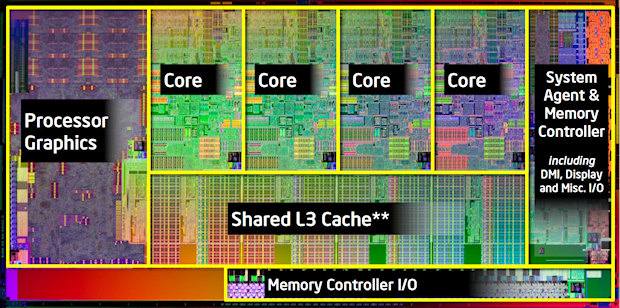
\includegraphics[scale=0.5]{sandy}
  \end{center}
  \caption{
    The figure depicts a quad-core Sandy Bridge microprocessor (or chip). The
    author was unable to locate an image of an octa-core chip.
  }
  \label{fig:p5}
\end{figure}

\subsection{Interconnecting chips to form larger SMPs}

Multiple Sandy Bridge chips can be connected to form larger modules in SMP
configurations. On Vilje, two chips are run in SMP mode on each compute node.
Thus, up to 16 (32) processors share memory.

\subsection{Interconnecting nodes to form a distributed SMP}

Multiple nodes may also be connected to form clusters or distributed SMPs. In
this case, data from one node to another must be passed across a high bandwidth
low-latency switch network. A system based on multiple nodes must therefore be
treated as a distributed memory system (at least globally).

\subsection{Key data for Vilje}

Vilje is based on 1404 nodes. The total number of processors (or cores) is
therefore 22464.

Each node represents a shared memory system with 2 octa-core Sandy Bridge chips
which share 32 GB memory (although a few nodes have 128 GB memory).

Each i7 processor operates at a clock rate of 2.6 GHz. The size of the L1 cache
(3 clocks) is 32 kbyte for data and 32 kbyte for instructions. The size of the
L2 cache (8 clocks) is 256 kbyte, while the size of the shared off-chip L3 cache
is 20 Mbyte.

\section{Programming models}

We have seen that a node (with 16 physical processors) on Vilje represents a
shared memory system where the aggregate memory for the node is globally
available to all the 16 processors. A shared memory programming model (i.e.
OpenMP) can therefore be used within a single node.

If we want to develop programs which can run on more than one node, we need to
use message-passing (i.e. MPI). This is also the programming model we will
emphasize in this course. Even though each node represents a shared memory
system, the message-passing programming model may still be used within a node.
However, the opposite is not true: a shared programming model cannot be used on
a ``pure'' distributed memory system (e.g. on a PC cluster).

Note that a system like Vilje, which represents a shared memory system within a
node, and a distributed memory system across the nodes, can also be programmed
using both programming models within a single program.


%-------------------------------------------------------------------------------
\newpage
\section{Distributed Memory Model: Message Passing}

Message passing is fundamentally processor-to-processor communication. Only a
local, unique memory is directly available to each processor. Both local and
remote processes must cooperate in order to exchange data and/or synchronize (at
least originally---some changes have been made in the extended version MPI-2).

Note that message-passing is a good way to use distributed shared memory
machines (ccNUMA) because it provides a way to express memory/data locality.

Some of the key advantages of the message-passing model are:
\begin{itemize}
\item {\em Portability}: the model can be used on a collection of
homogeneous or heterogeneous processors connected by a fast or a slow
communication network;
\item {\em Performance}: the approach exploits data locality, as well as the
availability of a large, aggregate memory;
\item {\em Expressiveness}: a limited communcation library suffices for most applications.
\end{itemize}

The Message Passing Interface (MPI) is the de facto standard for message
passing. It is a \emph{library}, not a language. MPI provides efficiency,
portability and functionality. It represents a standardized communcation library
running on a vast number of machines and architectures.
\autoref{fig:message_passing_model} illustrates the message passing model.

The original (1994) MPI-library represents the message passing model where both
the local and remote processes cooperate e.g. via a send and receive
operation. MPI-2 represents an extension of MPI where features like one-sided
messages, parallel I/O, etc. are included.

\begin{figure}
  \centering
  \begin{tikzpicture}[
  proc/.style={shape=circle, draw=darkblue, fill=cadet, thick},
  msg/.style={shape=rectangle, draw=darkblue, fill=cadet, thick, rounded corners=0.5mm},
  env/.style={minimum height=1.7cm, minimum width=1.7cm},
  scale=0.7,
  ]
  \node[proc] (p0) at (0,0) {$P_0$};
  \node[proc] (p1) at (1,3) {$P_1$};
  \node[proc] (p2) at (3,-0.6) {$P_2$};
  \node[proc] (p3) at (6,3.6) {$P_3$};
  \node[msg] (msg) at (4.0, 1.5) {\scriptsize Message};
  \node[msg, env, fill=cadet!55] (env) at (8, -2.0) {};
  \node[msg, very thin] (body) at (8, -1.7) {\scriptsize Body};
  \node[below of=body, node distance=6mm] {\scriptsize Envelope};
  \draw[->, thick] (p2) edge[bend right] node [right] {} (msg);
  \draw[->, thick] (msg) edge[bend right] node [right] {} (p1);
  \draw[->, thick] (env) edge[bend right] node [right] {} (msg);

  \node[msg] (smp) at (-2,-2) {\scriptsize SMP};
  \draw[->, thick] (smp) edge[bend left] node [right] {} (p0);
\end{tikzpicture}

  \caption{
    The message passing model. A number of processes, $P_0, P_1, \ldots,
    P_{n-1}$, are coupled together via a fast or a slow communication network.
    Each process has a local and unique memory/cache, and each process is
    associated with a particular computational task. The individual processes
    must communicate via explicit message passing. A message consists of an
    ``envelope'' which contains sufficient information about whether and when to
    open the message, as well as information regarding how to interpret the
    ``body'' of the message (the actual data). Note that the message is the only
    means of exchanging data between the processes and/or syncronizing the
    processes.
  }
  \label{fig:message_passing_model}
\end{figure}

The MPI operations can be classified in a few types of operations:
\begin{itemize}
\item one-to-one;
\item one-to-all;
\item all-to-one;
\item all-to-all.
\end{itemize}
The first type is also referred to as point-to-point operations (send and
receive), while the last three types are collective operations.

When we here talk about ``all'', we generally mean all processes $P_0, P_1,
\ldots, P_{n-1}$ within a group of $n$ processes. Such a group defines a
\emph{communicator} and the particular process number is referred to as the
\emph{rank} within that communicator. The default is to let all processes be
members of the same (default) communicator. However, it is also possible to have
some of the processes be members of one communicator (or group), while others be
members of a different communicator. In this context, ``all'' means all the
processes \emph{within} a particular communicator.

Finally, the collective operations can be further broken down into the
following categories:
\begin{itemize}
\item data movement (broadcast; gather/scatter);
\item collective computation (max/min; sum; etc.).
\end{itemize}

We will later explain in more detail the various MPI operations. A good way to
learn MPI is by implementing a few simple examples. The whole library contains
about 125 functions. However, as few as 6 may suffice for some problems. You
only need to learn the functions needed for your particular problem. You may not
have to learn the details of the whole library even for advanced applications.

\subsection{An example}

We now discuss a brief example of a program where the MPI library is used. The
program listed below does the following: processor 0 sends a text message
``Hello, world'' to all the other processors. The other processors receive the
message and all processors print out the message together with the their own
process number.

Listings \ref{lst:mpi-hello-c} and \ref{lst:mpi-hello-fortran} show how this is
done in both C and Fortran.

\begin{lstlisting}[style=c, float, caption={Hello world MPI in C.}, label=lst:mpi-hello-c]
  #include <stdio.h>
  #include "mpi.h"

  int main(int argc, char **argv)
  {
    int rank, size, tag, i;
    MPI_Status status;
    char message[20];

    MPI_Init(&argc, &argv);
    MPI_Comm_size(MPI_COMM_WORLD, &size);
    MPI_Comm_rank(MPI_COMM_WORLD, &rank);

    tag = 100;

    if (rank == 0) {
      strcpy(message, "Hello, world");
      for (i = 1; i < size; i++) {
        MPI_Send(message, 13, MPI_CHAR, i,
                 tag, MPI_COMM_WORLD);
      }
    }
    else {
      MPI_Recv(message, 13, MPI_CHAR, 0,
               tag, MPI_COMM_WORLD, &status);
    }

    printf("node %d: %13s\n", rank, message);

    MPI_Finalize();

    return 0;
  }
\end{lstlisting}

\begin{lstlisting}[style=fortran, float, caption={Hello world MPI in Fortran.}, label=lst:mpi-hello-fortran]
  program hello
  include 'mpif.h'

  integer rank, size, ierror, tag, status(MPI_STATUS_SIZE)
  character(12) message

  call MPI_INIT(ierror);
  call MPI_COMM_SIZE(MPI_COMM_WORLD, size, ierror);
  call MPI_COMM_RANK(MPI_COMM_WORLD, rank, ierror);

  tag = 100;

  if (rank .eq. 0) then
    message = 'Hello, world'
    do i=1,size-1
      call MPI_SEND(message, 12, MPI_CHARACTER, i, tag,
                    MPI_COMM_WORLD, ierror)
    enddo
  else
    call MPI_RECV(message, 12 MPI_CHARACTER, 0, tag
                  MPI_COMM_WORLD, status, ierror)
  endif

  print*, 'node', rank, ':', message

  call MPI_Finalize(ierror)
  end
\end{lstlisting}

The output of the C version on the SGI Origin using $P=4$ and $P=8$ processors
is shown in Listings \ref{lst:mpi-hello-4} and \ref{lst:mpi-hello-8}.

\begin{lstlisting}[float, caption={Hello world MPI in C: $4$ processors.}, label=lst:mpi-hello-4]
  node 1: Hello, world
  node 3: Hello, world
  node 2: Hello, world
\end{lstlisting}

\begin{lstlisting}[float, caption={Hello world MPI in C: $8$ processors.}, label=lst:mpi-hello-8]
  node 5: Hello, world
  node 1: Hello, world
  node 7: Hello, world
  node 2: Hello, world
  node 3: Hello, world
  node 6: Hello, world
  node 4: Hello, world
\end{lstlisting}

Let us now comment on some of the statements here. We start with
\begin{lstlisting}[style=c]
  #include <stdio.h>
  #include "mpi.h"
\end{lstlisting}
The first statement is just a standard statement about including the header file
associated with string (character) operations and I/O. The second statement is
required if we want to use the MPI library in our program. In C, we need the
statement
\begin{lstlisting}[style=c]
  #include "mpi.h"
\end{lstlisting}
The equivalent statement in Fortran is
\begin{lstlisting}[style=fortran]
  include 'mpi.f'
\end{lstlisting}
The MPI header file provides basic MPI definitions and MPI data types.

The first MPI statement needs to be:
\begin{lstlisting}[style=c]
  MPI_Init(&argc, &argv);
\end{lstlisting}
This statement should only be called once. The last MPI statement is always
\begin{lstlisting}[style=c]
  MPI_Finalize();
\end{lstlisting}
This statement does not have to be the very last statement in your program, but
it needs to be the last MPI statement. It statement ensures a clean exit.

Note that the command line arguments are passed to the C version of
\texttt{MPI\_Init}. The corresponding Fortran version reads:
\begin{lstlisting}[style=fortran]
  call MPI_INIT(ierror);
\end{lstlisting}
Similar to a standard subroutine call in Fortran, a call to an MPI operation
also starts with \texttt{call}. The parameter \texttt{ierror} is an integer and
will return an error code in case something goes wrong. The C version also
returns an error code. Instead of the statement used in the program listed
above, we could alternatively have written
\begin{lstlisting}[style=c]
  errorcode = MPI_Init(&argc, &argv);
\end{lstlisting}
In this case, the variable \texttt{errorcode} (an integer) will contain an error
code if something goes wrong.

In general, any MPI statement in C has the format
\begin{lstlisting}[style=c]
  errorcode = MPI_Xxxxx(parameters...);
\end{lstlisting}
or simply
\begin{lstlisting}[style=c]
  MPI_Xxxxx(parameters...);
\end{lstlisting}
The particular MPI operation is given by ``Xxxxx'' where the name of the operation
always starts with a capital letter and the remaining letters are lower-case.
The number and type of parameters vary from operation to operation. For example,
\texttt{MPI\_Finalize} does not have any parameters at all.

In Fortran, any MPI statement has the format.
\begin{lstlisting}[style=c]
  call MPI_XXXXX(parameters..., ierror)
\end{lstlisting}
where the parameter \emph{ierror} returns an error code. Note that the name of
the particular MPI operation is always in capital letters.

The next two statements after the initialization of MPI are:
\begin{lstlisting}[style=c]
  MPI_Comm_size (MPI_COMM_WORLD, &size);
  MPI_Comm_rank (MPI_COMM_WORLD, &rank);
\end{lstlisting}
The first of these statements returns the total number of MPI processes, while
the second one returns the individual process number (the ``rank''). More
precisely, the process number is stored in the location pointed to by the second
argument. \texttt{MPI\_COMM\_WORLD} is the default name of the communicator (the
``univertse'') and which include all the processes. This can be changed in order
to create several separate ``universes.''

Note that the program listed in this example runs separately and independently
on every processor on a multiprocessor. We also refer to this as SPMD -
\emph{Single Program Multiple Data}. All the problems we will study in this
course will be of this type: the program running on each processor will be the
same for all the processors. However, the data each processor will operate on
will typically be different. The synchronization of the program will be implicit
via the MPI operations. We will return to this issue later.

When this program runs on a particular processor, the program does not
automatically know how many other processors are involved; this issue is taken
care of by the MPI operation \texttt{MPI\_Comm\_size}. In the multiprocess
context, the program running on an individual processor does not automatically
know what its associated process number is (who am I?); this issue is taken care
of by the MPI operation \texttt{MPI\_Comm\_rank}.

Let us now proceed to the statements
\begin{lstlisting}[style=c]
  if (rank == 0) {
    strcpy (message, "Hello, world");
\end{lstlisting}
The if-statement will only be true for one of the processes, namely, the process
with process number 0. This is also referred to as the ``root'' process. On the
root process, the string ``Hello, world'' is copied into the string variable
\texttt{message}.

For all the other processes, the if-statement will not be true, and the program
execution will move on to the MPI statement \texttt{MPI\_Recv}. This means that
all of the other processes will be waiting for the root process to send them
data. The root process sends data to the other processes in the loop
\begin{lstlisting}[style=c]
  for (i=1; i < size; i++) {
    MPI_Send(message, 13, MPI_CHAR, i,
             tag, MPI_COMM_WORLD);
  }
\end{lstlisting}
Several comments are in order here. First, note that the root process sends out
the same message (string) to all the other processes. This is done in a loop.
However, note that this loop corresponds to a \emph{sequential} execution
meaning that a message will be sent to process $1$ before process $2$ etc.

Let us now discuss the particular format in the parameter list for the operation
\texttt{MPI\_Send}. The general format for this operation is
\begin{lstlisting}[style=c]
  MPI_Send(start, count, datatype, dest, tag, comm);
\end{lstlisting}
The first three parameters (start, count, datatype) represent \emph{the data},
while the last three parameters (dest, tag, comm) represent \emph{the envelope};
see \autoref{fig:message_passing_model}.

We now explain all these parameters in some more detail.
\begin{itemize}
\item \emph{start}: initial address of the send buffer
\item \emph{count}: number of elements sent (of type \texttt{datatype})
\item \emph{datatype}: e.g. \texttt{MPI\_INT}, \texttt{MPI\_FLOAT}, \texttt{MPI\_CHAR} etc.
\item \emph{dest}: destination process (integer)
\item \emph{tag}: integer message identifier (e.g., \texttt{MPI\_ANY\_TAG})
\item \emph{comm}: an ordered group of communication processes (same for send
  and receive)
\end{itemize}

Only the root process sends a message. All the other processes are waiting to
receive a message. This is expressed by the MPI operation \texttt{MPI\_Recv}.
The general format for this operation is
\begin{lstlisting}[style=c]
  MPI_Recv(start, count, datatype, source, tag, comm, &status);
\end{lstlisting}
The first three parameters (start, count, datatype) represent \emph{the data},
while the last three parameters (dest, tag, comm, status) represent \emph{the
envelope}; again, see \autoref{fig:message_passing_model}.

Most of the parameters are similar to the MPI\_Send operation:
\begin{itemize}
\item \emph{start}: initial address of the receive buffer
\item \emph{count}: number of elements sent (of type \emph{datatype})
\item \emph{datatype}: e.g. \texttt{MPI\_INT}, \texttt{MPI\_FLOAT}, \texttt{MPI\_CHAR} etc.
\item \emph{source}: source process (integer), i.e., the process sending the message
\item \emph{tag}: integer message identifier (e.g., \texttt{MPI\_ANY\_TAG})
\item \emph{comm}: an ordered group of communication processes (same for send and receive)
\item \emph{status}: a structure providing information on the completed communication
\end{itemize}

Note that in the small example program, an explicit source is given, namely, the
root process. Alternatively, we could have used \texttt{MPI\_ANY\_SOURCE} since
each process in receive mode only expects one message. Similarly, we note that
the ``tag'' is explicitly given. Alternatively, we could have used
\texttt{MPI\_ANY\_TAG} since this parameter is not critical in our case.

One additional comment regarding the send and receive statements. This is an
example of point-to-point communication. There exists several versions of send
and receive. The type used here is called \emph{blocking} send and receive. This
means that the program running on the root processor cannot proceed until each
message has been safely sent and the send buffer can be safely used again.
Similarly, the program running on each of the other processors cannot proceed
until the expected message has been received in the receive buffer.

Let us now comment on the parameter \emph{count} used in the send and receive
statements. In the C version, the count parameter is set equal to 13, while it
is 12 in the Fortran version. The reason for this is that the \texttt{strcpy}
function in C will append \texttt{\textbackslash 0} (the null character) at the
end of the message. This is a symbol which indicates the end of the string. Even
though ``Hello, world'' comprises 12 letters (one byte per letter), the message
buffer in C requires 13 bytes of memory.

The parameter ``datatype'' in the send and receive operations has to be the same.
In this case, the type is \texttt{MPI\_CHAR} (in Fortran the corresponding data
type is called \texttt{MPI\_CHARACTER}). This is one of several predefined data
types. Other important ones include \texttt{MPI\_DOUBLE} and \texttt{MPI\_INT}.

Finally, note that the output from the programs is not in a sequential order.
The order may also change if we run the program over again.


%-------------------------------------------------------------------------------
\newpage
\input{04-share-memory-model}

%-------------------------------------------------------------------------------
\newpage
\chapter{Basic linear algebra performance}

\section{Introduction}

Simulation-based science and technology require a rich set of numerical
algorithms. For example, in the context of numerical solution of partial
differential equations we have seen the need to solve linear systems of
algebraic equations. Solution algorithms for linear system of equations may
again be classified as direct methods or iterative methods. In either case, the
solution algorithms rely on basic linear algebra operations. Most of the
floating point operations in a typical simulation code are associated with such
operations.

Because of the importance of basis linear algebra operations, a special library
called BLAS (\emph{Basic Linear Algebra Subroutines}) has been developed to deal
with such operations. The BLAS library is again classified into three levels:
\begin{itemize}
\item Level 1 operations: vector-vector operations;
\item Level 2 operations: matrix-vector operations;
\item Level 3 operations: matrix-matrix operations.
\end{itemize}
Two examples of level 1 BLAS operations are
\begin{align}
  \bm y := a \bm x + \bm y
  \label{eq:daxpy}
\end{align}
and
\begin{align}
  \sigma = \bm x \cdot \bm y = \bm x^\intercal \bm y
  \label{eq:dot}
\end{align}
Operation \eqref{eq:daxpy} is called a {\em daxpy} operation. Here, the input
$\bm x$ of length $n$ is scaled with a constant $a$ and added to the second
input vector $\bm y$, which is also of length $n$. The result is then stored
back in the vector $\bm y$, i.e. the original values in $\bm y$ are overwritten.

Operation \eqref{eq:dot} represents a dot product (or inner product) which we
have discussed extensively earlier in the course. Here, from the two input
vectors $\bm x$ and $\bm y$ (both of length $n$) we compute the scalar $\sigma$.

An example of a level 2 BLAS operation is the matrix-vector product
\begin{align}
  \bm y = \bm A \bm x
  \label{eq:mvp}
\end{align}
Here, the output vector $\bm y$ (of length $m$) is computed from the given input
matrix $\bm A$ (of dimension $m \times n$) and the given input vector $\bm x$
(of length $n$).

An example of a level 3 BLAS operation is the matrix-matrix product
\begin{align}
  \bm C = \bm A \bm B
  \label{eq:mxm}
\end{align}
Here, the matrix $\bm X$ (of dimension $m\times n$) is computed as the product
of the matrix $\bm A$ (of dimension $m\times k$) and the matrix $\bm B$ (of
dimension $k\times n$).

In this set of lecture notes, we will discuss the performance of operations
\ref{eq:daxpy}, \ref{eq:dot} and \ref{eq:mxm} on Vilje. We will primarily focus
on the single-processor performance, but we will also consider the
multi-processor performance using the BLAS implementation included in the MKL
library developed at Intel.

In particular, we will discuss the performance as a function of:
\begin{itemize}
\item basic linear algebra operation;
\item programming aspects;
\item high level programming languages;
\item exploiting multiple threads.
\end{itemize}

\subsection{Key data for Vilje}

The current supercomputer at NTNU, Vilje, is based on 1404 nodes. The total
number of processors (or cores) is 22464 physical cores, each core being
hyperthreaded, thus having 44928 logical cores.

Each node represents a shared memory system with 2 octave-core Sandy Bridge
chips which share 32 GB memory (although a few nodes have 128 GB memory).

Each processor operates at a clock rate of 2.6 GHz. The size of the private L1
cache is 32 kbyte for data and 32 kbyte for instructions. The size of the
private L2 cache is 256 kB, while the size of the off-chip L3 cache is 20 Mbyte.

The latency associated with the different memory levels is: 8 clock cycles for
L2, 30 clock cycles for L3, and 150 clock cycles for main memory.

\subsection{Maximum theoretical performance}

The maximum theoretical performance (or peak performance) is the maximum number
of floating point operations completed per second. We may talk about the maximum
theoretical performance for a single CPU, a single node, or for the entire
machine.

The maximum theoretical performance of a single core of a Sandy Bridge chip is
found as follows. First, each physical has a separate SIMD floating point unit
(AVX). This is a superscalar/FMA capable (Fused Multiply and Add) vector unit
which can operate on 4 double precision number simultaneously. This performance
is achieved if the units can be filled fast enough with data, and after a
certain start-up period (recall the earlier discussion about pipelining). With 1
AVX per physical core, the maximum theoretical performance per core is thus 8
floating point operations per clock cycle. With a clock cycle of 2.6 GHz, this
translates into 21 Gflops per physical core. Note, since logical cores share AVX
units, we cannot expect additional performance from using the hyperthreads,
since in order to achieve this performance we are already using the full memory
bandwidth of the machine.

Unfortunately, many operations only achieve a fraction of the maximum
theoretical performance. The measured performance will typically depend on the
the reuse of data (a high degree of reuse means less memory traffic) and how
good the compiler is. For the basic linear algebra operations we will study
here, we will see a large variation in performance. Not surprisingly, the
specially developed BLAS library will typically give excellent performance.
However, some of the observed differences may come as a surprise.

\section{Compiling and running the programs}

The source code and the buildsystem for the tests are found in the git
repository at \url{https://github.com/TheBB/TMA4280}, in the
\url{code/performance} directory. CMake is used to generate the different
Fortran programs, and to generate a build system capable of building the testing
suite on most machines, including Vilje or your local Linux/OSX machine. There
is also a example job script, a script to postprocess the results and (for those
interested) the Octave/Matlab scripts used to generate the \LaTeX~code for the
tables in this document.

\section{Vector-vector operations}

In this section we briefly discuss some performance results for an important
vector-vector operation: the daxpy-operation \eqref{eq:daxpy}, which named as
such: \textbf{d}ouble precision \textbf{a}lpha $\bm x$ \textbf{p}lus $\bm y$.
\[
  \bm y := \alpha \bm x + \bm y,
\]
does exactly $n$ operations (additions) on $\mathcal{O}(n)$ data, and needs to
store $n$ floating point numbers back into memory. All this memory traffic will
severely influence the performance we can reach. In contrast to the
matrix-matrix multiplication, only $\mathcal{O}(1)$ floating point operations
are needed per floating point number stored. There is thus very little "reuse"
of data in vector-vector operations. From these general considerations we expect
vector-vector operations to perform significantly worse than the matrix-matrix
product multiplication.

\subsection{Performance results for daxpy}

\Autoref{tab:tab9, tab:tab10} show the performance results of the daxpy
operation. In general, a standard implementation of the daxpy operation in C
(i.e., a single loop), performs just fine. This is to be expected since this
operation is utterly memory bandwidth bound and not much can be done wrong.

\begin{table}
  \caption{
    Performance results (in MFlops) for a standard daxpy implementation in C
    (implemented as a single loop), compared with the performance using BLAS.
  }
  \label{tab:tab9}
  \begin{center}
  \bgroup\def\arraystretch{1.2}
  \begin{tabular}{c|rrrr|r}
    \hline
    $n$ & \texttt{-O0} & \texttt{-O1} & \texttt{-O2} & \texttt{-O3} & BLAS \\
    \hhline{======}
    $10^2$ & 45.92 & 63.69 & 82.82 & 68.37 & 0.10 \\
    $10^3$ & 227.13 & 363.00 & 457.12 & 434.61 & 0.81 \\
    $10^4$ & 403.55 & 1122.64 & 1217.60 & 1246.42 & 7.76 \\
    $10^5$ & 415.85 & 1300.58 & 1322.22 & 1338.98 & 79.71 \\
    $10^6$ & 379.52 & 418.88 & 413.65 & 413.65 & 341.52 \\
    $10^7$ & 376.78 & 420.55 & 413.65 & 420.36 & 341.52 \\
    \hline
  \end{tabular}
  \egroup
\end{center}

\end{table}

\begin{table}
  \caption{
    Performance results (in MFlops) for a standard daxpy implementation in
    Fortran (implemented as a single loop), compared with the performance using
    BLAS.
  }
  \label{tab:tab10}
  \begin{center}
  \bgroup\def\arraystretch{1.2}
  \begin{tabular}{c|rrrr|r}
    \hline
    $n$ & \texttt{-O0} & \texttt{-O1} & \texttt{-O2} & \texttt{-O3} & BLAS\\
    \hhline{======}
    $10^2$ & 0.07 & 0.07 & 0.08 & 0.07 & 0.10 \\
    $10^3$ & 0.89 & 0.83 & 0.67 & 0.69 & 0.80 \\
    $10^4$ & 9.37 & 7.23 & 8.17 & 7.30 & 7.75 \\
    $10^5$ & 70.96 & 66.18 & 70.65 & 87.33 & 79.70 \\
    $10^6$ & 353.27 & 356.28 & 385.78 & 402.52 & 341.51 \\
    $10^7$ & 513.54 & 514.07 & 514.52 & 512.66 & 341.51 \\
    \hline
  \end{tabular}
  \egroup
\end{center}

\end{table}

\section{Matrix-matrix multiplication}

Let us first consider the matrix-matrix multiplication \eqref{eq:mxm}. In
general, if $\bm A \in \mathbb{R}^{m \times k}$, $\bm B \in \mathbb{R}^{k \times
n}$ and $\bm C \in \mathbb{R}^{m \times n}$,
\[
  c_{ij} = \sum_{l=1}^k a_{il}b_{lj}, \qquad
  \forall\ i=1,\ldots,m, \qquad
  \forall\ j=1,\ldots,n.
\]
Written out, this is
\[
  c_{ij} = a_{i1}b_{1j} + a_{i2}b_{2j}+\cdots+a_{ik}b_{kj} \qquad
  \forall\ i=1,\ldots,m, \qquad
  \forall\ j=1,\ldots,n.
\]
Mathematically, there are thus $k$ multiplications and $k-1$ additions for each
index $i,j$. The total number of operations is then
\[
  \mathcal{N}_\text{op} = mn\left(2k-1\right).
\]

For the special case where $A,B,C\in \mathbb{R}^{nxn}$, the total number of operations is
\[
  \mathcal{N}_\text{op} = n^2²\left(2n-1\right) \approx 2n^3.
\]
Hence, if $m,n,k$ are of the same order (e.g., $m=k=n$),
\begin{align}
  \mathcal{N}_\text{op} = \mathcal{O}(n^3).
\end{align}

\subsection{Triple-nested loop}

In a numerical program, matrix multiplication can be implemented in several ways.
The most straightforward method is in a triple-nested loop as follows (using C).
\begin{lstlisting}[style=c]
  for(i=0; i<m; i++) {
    for(j=0; j<n; j++) {
      c[i][j] = 0.0;
      for(l=0; l<k; l++) {
        c[i][j] += a[i][l]*b[l][j];
      }
    }
  }
\end{lstlisting}
Here, the terms are accumulated relative to an initialized value of zero.
Counting the number of floating point operations in the inner-most loop, there
are one multiplication and one addition. The total number of floating point
operations for matrix multiplication then becomes $\mathcal{N}_\text{op} = 2mnk$
( $=2n^3$ when $m=k=n$).

\subsection{Loop unrolling}

Loop unrolling helps to make the data flow and the data dependencies more
explicit and prepare for good use of the floating point units. For example, when
$k=10$, the inner-most loop can be unrolled manually to get the following
alternative version:
\begin{lstlisting}[style=c]
  for (i=0; i<m; i++) {
    for (j=0; j<n; j++) {
      c[i][j] = a[i][0]*b[0][j]
              + a[i][1]*b[1][j]
              + a[i][2]*b[2][j]
              + a[i][3]*b[3][j]
              + a[i][4]*b[4][j]
              + a[i][5]*b[5][j]
              + a[i][6]*b[6][j]
              + a[i][7]*b[7][j]
              + a[i][8]*b[8][j]
              + a[i][9]*b[9][j];
    }
  }
\end{lstlisting}
Here, all the terms are written out explicitly, following the mathematical
definition. The computation of \texttt{c[i][j]} now takes one addition fewer.

Loop unrolling reveals independent operations that can be performed
concurrently, while reducing the index-related overhead of the loop. This makes
it possible to make better use of the pipelined, superscalar (vector) floating
point units of the processor. At high enough optimization levels, the compiler
will typically try to unroll loops where it sees this as beneficial.

\subsection{Performance results}

We now present performance measurements for the matrix-matrix multiplication.
The source codes used are given in the appendix. In all the tests we perform,
$m=k=n$ (i.e., we consider square matrices). Both a C version and a Fortran
version of the matrix-matrix operation will be tested and compared with the
performance using the \texttt{dgemm} routine from the BLAS library. We provide
the full program listings, together with a description of how the programs were
compiled and run on Vilje. For example, we will explore the effect of using
different levels of compiler optimization.

Note that we may call the Level 3 BLAS routine \texttt{dgemm} from either
Fortran or C. When we use this library routine, the optimization level or code
language should not matter. As long as $n$ is large enough, it is possible to
obtain a high degree of peak performance.

Finally, note that the performance results we list in the following are
approximate and may not be exactly reproducable. However, they represent typical
results and the conclusions we arrive at should be valid.

The programs were run on 16 processors even though the code contains no
communication between the processors. This gave 16 timing results per run.

These versions are single threaded; the difference is only the compiler
optimization level.

\begin{table}
  \caption{Standard mxm (triple-nested loop) using C, compared with BLAS.}
  \label{table:tab1}
  \begin{center}
  \bgroup\def\arraystretch{1.2}
  \begin{tabular}{c|rrrr|r}
    \hline
    $n$ & \texttt{-O0} & \texttt{-O1} & \texttt{-O2} & \texttt{-O3} & BLAS \\
    \hhline{======}
    100 & 274.55 & 566.00 & 562.76 & 563.32 & 775.64 \\
    500 & 226.53 & 503.96 & 496.40 & 496.84 & 14323.68 \\
    1000 & 180.78 & 214.33 & 214.37 & 214.36 & 16786.90 \\
    1500 & 169.95 & 205.26 & 204.69 & 204.55 & 17808.83 \\
    \hline
  \end{tabular}
  \egroup
\end{center}

\end{table}

As can be seen from \autoref{table:tab1}, the compiler optimization level had
really disappointing influence on the obtained performance---in fact, it
actually reduced it in some cases. These results looks far from flattering for
the C programming language. Fortunately, this can be overcome by using BLAS, in
this case through MKL. The BLAS version of the program was invoked by calling
e.g.

\begin{lstlisting}[style=shell]
  mpirun -np 16 timing-O3 1000 2
\end{lstlisting}

For the Fortran version of the programs, however, as can be seen from
\autoref{table:tab2}, the compiler optimization level greatly influences the
obtained performance.

\begin{table}
  \caption{
    Standard $m \times m$ (triple-nested loop) using Fortran, compared with
    BLAS.
  }
  \label{table:tab2}
  \begin{center}
  \bgroup\def\arraystretch{1.2}
  \begin{tabular}{c|rrrr|r}
    \hline
    $n$ & \texttt{-O0} & \texttt{-O1} & \texttt{-O2} & \texttt{-O3} & BLAS \\
    \hhline{======}
    100 & 247.37 & 1666.47 & 4800.47 & 7109.23 & 775.64 \\
    500 & 191.22 & 982.85 & 3375.70 & 7565.13 & 14323.68 \\
    1000 & 142.11 & 210.15 & 1356.46 & 7228.42 & 16786.90 \\
    1500 & 122.92 & 205.13 & 1357.79 & 7584.47 & 17808.83 \\
    \hline
  \end{tabular}
  \egroup
\end{center}

\end{table}

We see that the language utilized greatly influnces the performance of this
operation. This can be attributed to the fact that, given proper memory
handling, the matrix times matrix operation is dominated by floating point
operations. The BLAS and (and to some extent) Fortran realizations manage to
keep the pipelines filled with data, while the C version does not seem to be
able to keep the floating point units fully occupied.

Let us also compare these performance results with the manually unrolled
innermost loop (which we have done for the specific case $n=10$). The programs
are compiled and linked as before. When we activate \texttt{mxm\_unr}, we obtain
the results in \Autoref{table:convergence_C, table:convergence_F}.

\begin{table}
  \caption{``Manually'' unrolled innermost loop (\texttt{mxm\_unr}), C.}
  \label{table:convergence_C}
  \begin{center}
  \bgroup\def\arraystretch{1.2}
  \begin{tabular}{c|rrrr}
    \hline
    $n$ & \texttt{-O0} & \texttt{-O1} & \texttt{-O2} & \texttt{-O3} \\
    \hhline{=====}
    10 & 328.19 & 485.23 & 577.84 & 409.26 \\
    \hline
  \end{tabular}
  \egroup
\end{center}

\end{table}

\begin{table}
  \caption{``Manually'' unrolled innermost (\texttt{mxm\_unr}), Fortran.}
  \label{table:convergence_F}
  \begin{center}
  \bgroup\def\arraystretch{1.2}
  \begin{tabular}{c|rrrr}
    \hline
    $n$ & \texttt{-O0} & \texttt{-O1} & \texttt{-O2} & \texttt{-O3} \\
    \hhline{=====}
    10 & 189.17 & 292.61 & 674.69 & 621.29 \\
    \hline
  \end{tabular}
  \egroup
\end{center}

\end{table}

We do not observe much performance increase for either case. It seems that this is a trick
the compiler uses extensively on its own. Note that the Fortran version is still
about 50\% faster than the C version (for \texttt{-O3}).

We now try to use the parallel (multi-threaded version) of BLAS implemented in
the MKL library.
\begin{table}
  \caption{BLAS with 16 threads (SMP). All performance numbers are in MFlops.}
  \label{table:tab4}
  \begin{center}
    \bgroup\def\arraystretch{1.2}
    \begin{tabular}{cr}
      \hline
      $n$ & BLAS (16 threads) \\
      \hhline{==}
      100 & 1463.80 \\
      500 & 66599 \\
      1000 & 100527 \\
      1500 & 101389 \\
      \hline
    \end{tabular}
    \egroup
  \end{center}
\end{table}

From \autoref{table:tab4} we see that we obtain very impressive performance.
These numbers should be compared with the maximum theoretical performance for
the entire node (i.e., using 16 processors) which is $16\times 21$ GFlops $=
336$ GFlops. Note that the cannot get more than 21 GFlops per core since this
number corresponds to the maximum performance of the available multiply-and-add
units per core. We thus see that BLAS (using the SMP version of the \texttt{MKL}
library) achieves close to 33\% of the maximum theoretical performance over 16
processors. This is actually quite impressive since this was achieved only by
adding a few compile and run flags; the program itself is unchanged from
earlier. This might seem a bit disappointing, but it just shows the real
bottleneck in the computer: memory bandwidth.

Finally, we recall the reason for the excellent performance of the BLAS library
for the matrix-matrix multiplication operation: the mxm operation uses
$\mathcal{O}(n^2)$ data and $\mathcal{O}(n^3)$ operations, implying that we need
to do $\mathcal{O}(n)$ floating point operations per single floating point
number stored. Because of the significant "reuse" of data, there is a
significant potential to hide the memory latency and keep the floating point
units busy. In particular, BLAS is able to get close to optimal single-processor
performance, and a standard triple loop in Fortran is able to get fairly close
using two threads per core. Unfortunately, the C version is not able to keep the
floating point units busy enough.

\subsection{Combining Fortran and C}

We recall that memory is allocated column-wise in Fortran and row-wise in C. In
BLAS the Fortran convention is used. It is thus necessary to be careful when
using two-dimensional arrays when calling \texttt{dgemm} (or other routines
following the Fortran convention).

To ensure correctness, there are several ways to proceed. By switching indices
when accessing arrays in C, a ``pseduo'' column-wise allocation is achieved.
This is the approach we chose to use here (and in the rest of the course).
Sometimes it may be possible to use a version of the library that accepts
row-wise allocation, such as the CBLAS library. However, CBLAS is not as
universally available, so we have chosen the approach that is most portable.

% The standard inner product (or dot product) of two vectors $x$ and $y$
% of length $n$ is given by
% \[
%         \sigma = \underline{x}^T\underline{y} = \underline{x}\cdot \underline{y} =
%         \sum_{i=1}^n x_i y_i.
% \]
% This operation requires $\mathcal{O}(n)$ floating point operations
% ($n$ multiplications and $n-1$ additions) on
% $2n = \mathcal{O}(n)$ floating point numbers, and only a
% single number ($\sigma$) needs to be stored back to memory.

% \begin{figure}
% \centering
%         \subfigure[Fortran]{\includegraphics[width=10cm]{daxpy-smp-fortran}}\\
%         \subfigure[BLAS]{\includegraphics[width=10cm]{daxpy-smp-blas}}
%         \caption{Performance of the daxpy operation in SMP mode. All programs are compiled with full compiler optimizations.}
%         \label{fig:daxpy-smp}
% \end{figure}
% \input{Table12.tex}

% \subsection{Performance results: inner product}

% Tables 7-10 show the performance of the inner product on \texttt{njord}.

% \begin{center}
  \bgroup\def\arraystretch{1.2}
  \begin{tabular}{c|rrrr|r}
    \hline
    $n$ & \texttt{-O0} & \texttt{-O1} & \texttt{-O2} & \texttt{-O3} & BLAS \\
    \hhline{======}
    $10^2$ & 45.92 & 63.69 & 82.82 & 68.37 & 0.10 \\
    $10^3$ & 227.13 & 363.00 & 457.12 & 434.61 & 0.81 \\
    $10^4$ & 403.55 & 1122.64 & 1217.60 & 1246.42 & 7.76 \\
    $10^5$ & 415.85 & 1300.58 & 1322.22 & 1338.98 & 79.71 \\
    $10^6$ & 379.52 & 418.88 & 413.65 & 413.65 & 341.52 \\
    $10^7$ & 376.78 & 420.55 & 413.65 & 420.36 & 341.52 \\
    \hline
  \end{tabular}
  \egroup
\end{center}

% \begin{center}
  \bgroup\def\arraystretch{1.2}
  \begin{tabular}{c|rrrr|r}
    \hline
    $n$ & \texttt{-O0} & \texttt{-O1} & \texttt{-O2} & \texttt{-O3} & BLAS\\
    \hhline{======}
    $10^2$ & 0.07 & 0.07 & 0.08 & 0.07 & 0.10 \\
    $10^3$ & 0.89 & 0.83 & 0.67 & 0.69 & 0.80 \\
    $10^4$ & 9.37 & 7.23 & 8.17 & 7.30 & 7.75 \\
    $10^5$ & 70.96 & 66.18 & 70.65 & 87.33 & 79.70 \\
    $10^6$ & 353.27 & 356.28 & 385.78 & 402.52 & 341.51 \\
    $10^7$ & 513.54 & 514.07 & 514.52 & 512.66 & 341.51 \\
    \hline
  \end{tabular}
  \egroup
\end{center}

% \begin{figure}
%         \includegraphics{inner}
%         \caption{Performance of the inner product operation in a single core,
%         single thread mode.
%         All programs are compiled with full compiler optimizations.
%         We now see that the specific programming language has less influence
%         on the performance compared to the matrix-matrix operation.
%         This can be attributed to the fact that a vector-vector operation
%         is latency bound and that the main aspect limiting the performance is
%         how fast the machine can feed the processor data.}
%         \label{fig:inner}
% \end{figure}

% \input{Table7.tex}
% \begin{figure}
%         \includegraphics{inner-smt}
%         \caption{Performance of the inner product operation in single core, SMT mode.
%         All programs are compiled with full compiler optimizations.
%         We now see that the specific programming language has less influence
%         on the performance compared to the matrix-matrix operation.
%         This can be attributed to the fact that a vector-vector operation
%         is latency bound and that the main aspect limiting the performance is
%         how fast the machine can feed the processor data.}
%         \label{fig:inner-smt}
% \end{figure}

% \input{Table8.tex}
% \begin{figure}
% \centering
%         \subfigure[FORTRAN]{\includegraphics[width=10cm]{inner-smp-fortran}}\\
%         \subfigure[BLAS]{\includegraphics[width=10cm]{inner-smp-blas}}
%         \caption{Performance of the inner product operation with $x \neq y$ in SMP mode. All programs are compiled with full compiler optimizations.}
%         \label{fig:inner-smp}
% \end{figure}


% \clearpage
% \subsection{Performance results: inner product (x=y)}

% Finally Tables 13-16 show the performance of an inner product
% when $x$ and $y$ is the same vector.

% \input{Table13.tex}
% \input{Table14.tex}
% \begin{figure}
%         \includegraphics{dot}
%         \caption{Performance of the inner product operation where $x = y$.
%                          All programs are compiled with full compiler optimizations.
%                          We see that this time the language utilized has less influnces
%                          on the performance of the operation. This can be attributed to the fact that this
%                          operation is latency bound and that the main thing limiting the performance is
%                          how fast the machine can feed the processor data.}
%         \label{fig:dot}
% \end{figure}
% \input{Table15.tex}
% \begin{figure}
%         \includegraphics{dot-smt}
%         \caption{Performance of the inner product operation where $x = y$ in SMT mode.
%                          All programs are compiled with full compiler optimizations.
%                          We see that this time the language utilized has less influnces
%                          on the performance of the operation. This can be attributed to the fact that this
%                          operation is latency bound and that the main thing limiting the performance is
%                          how fast the machine can feed the processor data.}
%         \label{fig:dot-smt}
% \end{figure}

% \input{Table16.tex}
% \begin{figure}
%         \subfigure[Fortran]{\includegraphics[width=6.5cm]{dot-smp-fortran}}
%         \subfigure[BLAS]{\includegraphics[width=6.5cm]{dot-smp-blas}}
%         \caption{Performance of the inner product operation where $x = y$ in SMP mode. All programs are compiled with full compiler optimizations.}
%         \label{fig:dot-smp}
% \end{figure}

% \end{document}

% \clearpage
% \section{Discussion}


% \subsection*{Memory limitations}
% In the vector-vector operation \emph{daxpy} a vector is multiplied with a scalar,
% and the result is added to another vector, overwriting the second vector. In Fortran
% language this will look like the following loop:
% \begin{lstlisting}[language=Fortran]
% real*8 a, x(n), y(n)
% do i = 1,n
%         y(i) = y(i) + a*x(i)
% enddo
% \end{lstlisting}
% Each iteration of the loop, the two elements $x(i)$ and $y(i)$ are loaded to registers,
% a multiply-add operation is performed on the data, and the result $y(i)$ is stored
% to memory. (In addition, some indexing work and a test for completion of the loop must be
% performed. The scalar constant a can be held in a register, without any need for extra
% memory operations.)

% The load/store unit can be used concurrently with the floating-point units.
% Each cycle, it can perform either a load or a store operation. At best,
% a store operatin in this example can be performed every third cycle, with two
% loads in between. Since the stored value is the result of one multiply-add operation,
% the maximum achievable performance for \emph {daxpy} is one third of peak performance.

% Figure \ref{fig:daxpy} demonstrates achievable performance of the daxpy operation on Njord.



% \subsection*{Data reuse in matrix multiplication}
% The key to higher performance than what was possible in the pervious example, is to perform
% more operations on the data that is being loaded, before storing the results.

% In matrix multiplication the amount of work is $\mathcal{O}\left(N^3\right)$, while the amount
% of data is $\mathcal{O}\left(N^2\right)$. Therefore, this problem has a potential for
% data resue. By rewriting the nested loop, the number of load and store operations
% can be reduce to the same as the nmber of multiply-add operations (or lower).

% The way this is accomplished is by performing outer loop unrolling. When this technique
% is used, a small block of values from one of the arrays is stored in registers for reuse.

% If both the outer loops are unrolled twice, the Fotran matrix multiplication
% loop would look similar to the following:
% \begin{lstlisting}
% do j = 1,n, 2
%         do l=1,k,2
%                 b00 = b(l,j)
%                 b01 = b(l,j+1)
%                 b01 = b(l+1,j)
%                 b11 = b(l+1,j+1)
%                 do i= 1,m
%                         c(i,j)   = c(i,j)   + a(i,1)  *b00
%                         c(i,j+1) = c(i,j+1) + a(i,1)  *b01
%                         c(i,j)   = c(i,j)   + a(i,1+1)*b10
%                         c(i,j+1) = c(i,j+1) + a(i,1+1)*b11
%                 enddo
%         enddo
% enddo
% \end{lstlisting}

% In the inner loop, there are now 6 memory operations (4 loads and 2 stores),
% whle there are 4 multiply-add operations. Four registers are needed to hold
% the constant array elements from the \emph{b} array. As the degree of unrolling
% increases, the number of memory operations can be reduced further. However,
% the number of available registers eventually becomes a bottleneck.

% The SGI compiler system has a Loop Nest Optimizer (LNO) module that
% performs outer loop unrolling at \emph{-O3} and higher, in an early
% compilation stage. The inner loop is unrolled if necessary in the final stages
% of the compilation, using so-called software pipelining principles.

% \subsection*{Cache optimizations}
% The outer loop unrolling enables the processor to reach performance levels
% close to the theoretical maximum, by converting the loop from memory
% bound to floating point bound. However, when the matrix dimension increases,
% performance will fall as lower levels of the memory hierarchy are accessed.

% The LNO module will use other forms of optimizations to improve cache and
% memory behavior. Loop interchange may enabled stride-1 acess to arrays.
% If the data structures are too big to fin in (usually) L2 cache, cache blocking
% is performed. The matrices or arrays are split into smaller pieces or blocks
% that fits in cache. The matrix multiplication is then performed in a series
% of sub-matrix multiplies.

% Another type of optimization the LNO module performs is prefetching. Data
% can be moved from meory into cache befroe use, hiding the meory acess
% time. In a similar way load operations can be performed as early as possible
% to hide the load latency from L1 cache.

% The combined effect of the optimizations performed by the LNO module can
% greatly enhance performance. However, it can be hard to understand the transformed
% version of a loop like the matrix multiplication.

% \subsection*{Measured performance of matrix multiplication}
% The most obvious factor in performance is the matrix dimension. For $n=10$,
% high overhead costs can make performance sub-optimal. For $n=100$, and
% particular $n=500$, a good version of the code will be able to achieve
% high performance, as the data fits in L2 cache.

% As the matrix dimensions approaches 600, there is an increasing pressure
% on L2 cache. At $n=1000$, the performance will to a large degree be a measure
% of how effective the cache optimization techniques have been.

% Except for the smallest problem size, \emph{dgemm} delivers high performance.
% The BLAS library is optimized for problems sizes that needs good use of the lower
% levels of the memory herarchy. BLAS exists for all platforms used in scientific
% computing, and is often tuned by the system vendor using automated optimization techniques.

% For smaller problem sizes, the best performance may be achieve by the
% compiler, by carefully writing an unrolled or cache blocked version, or by a
% combination of these. The Fortran compiler was able to produce code that
% gave high performance for a range of problems sizes. The manually unrolled versions
% had decent performance as well.

% \subsection*{Language differences}
% It is apparent that the Fortran version of the code delivers much higher
% performance than the C version. The reason is inherent difficulties with optimization
% of C code. While performing optimizations, the particular optimal scheduling of
% instructions in an inner loop, the compiler bust be certain that the correctness of results
% are not effected.

% The use of pointers in C introduces a difficulty for the compiler. Two pointer
% variables may in principle refer to identical memory locations. There is no way
% for the compiler to know whether such aliasing does in fact occur. It is possible
% to specify that pointers do not point to overlapping regions of memory.

% For the \emph{daxpy} operation, this made it possible to achieve equal performance
% levels under C and Fortran. For the matrix multiplication, the C version showed
% improved performance using this compiler option, but the results
% were still not as good as under Fortran. This probably had to do with the use of
% two-dimentional arrays.

% \subsection*{Pitfalls when combining Fortran and C}
% Memory is allocated column-wise in Fortran and row-wise in C. In the BLAS library
% the Fortran convention is used. It is necessary to be careful when using two-dimensional
% arrays when call \emph{dgemm} (or other routines following the Fortran convention).

% To ensure correctness, there are several ways to proceed. By switching indices
% when accessing arrays in C, a ``pseduo'' column-wise allocation is achieved.
% Sometimes it may be possible to use a version of the library that accepts row-wise
% allocation, such as the CBLAS library.

% It is also possible to rewrite the original matrix computation using transposed terms.
% This was done in the C version here. Since \emph{dgemm} can handle transposed arrays,
% in reality we used dgemm to compute $C^T = A^T\cdot B^T$.

% \subsection*{Conclusion}
% The matrix multiplication operation is an interesting problem in numerical programming.
% In principle, it may deliver high performance, by exploiting
% the potential of data reuse. However, this will not happen automatically. An
% implementation that is performing well fro some problem sizes, may not be appropriate
% for others.

% One option is to use the \emph{dgemm} routing from the BLAS Level 3 library. This may in
% particular be a good choice for large matrices. Figure \ref{fig:mxm} demonstrates
% that the compiler may produce fast code for a range of matrix dimensions that is L2 cache friendly.
% However, this may be language dependent.

% The compiler was able to produce very fast code from the simple Fortran triple-nested loop.
% Often bloated code is slow code. However, for the smallest problem sizes, it is possible
% to demonstrate that a carefully manually unrolled version delivers even better performance,
% even though it is using many lines of code (This is not shown here.) Performance measurements
% can help decide what will be the right way to implement a routine such as matrix multiplication.


%-------------------------------------------------------------------------------
\newpage
\chapter{The Poisson problem}

\section{The Poisson problem}

The Poisson problem typically models a diffusion process, and is a very
important model problem in science and engineering. This is related to the fact
that the Poisson problem may constitute the whole, or more commonly, part of a
mathematical model describing a physical system.

Numerical algorithms for solving partial differential equations often decouple a
complex problem into subproblems, of which the Poisson problem is an important
one.

We now give a few examples. We start by considering the Poisson equation
\begin{align}
  \label{poisson-eq}
  - \nabla^2 u = f
\end{align}
defined in a domain $\Omega$.

A physical example where this type of equation represents the governing equation
can be found in electrostatics. In this case, the differential forms for the
electric field $\bm $ are
\begin{align}
\nabla \cdot  {\bm E} &= 4 \pi \rho,\\
\nabla \times {\bm E} &= 0,
\end{align}
where $\rho$ is the charge density. It follows that the electric field
$\bm E$ can be expressed as the gradient of a scalar field
$\phi$, i.e., ${\bm E}= - \nabla \phi$. Hence,
\begin{align}
  \nabla \cdot  {\bm E} =
  - \nabla \cdot \nabla \phi = - \nabla^2 \phi = 4 \pi \rho.
\end{align}

The Poisson equation \eqref{poisson-eq} is an example of an elliptic partial
differential equation. It is typically solved on a bounded domain $\Omega$, in
which case we need to specify boundary conditions for $u$ on the domain boundary
$\partial \Omega$, e.g., the potential function $\phi$ defined on $\partial
\Omega$. Note that the potential $\phi$ at any point in the domain $\Omega$ will
depend on the specified potential along the entire boundary $\partial \Omega$.

A similar example is the potential flow approximation in fluid mechanics. If the
velocity field $\bm U$ is irrotational and incompressible, i.e.
\begin{align}
  \nabla \times {\bm U} &= 0, \\
  \nabla \cdot  {\bm U} &= 0,
\end{align}
it follows that ${\bm U}= \nabla \phi$, where $\phi$ represents a scalar
velocity potential and satisfies the Laplace equation
\begin{align}
  \nabla^2 \phi = 0.
\end{align}

A third example where the Poisson equation represents the governing equation is
{\em steady} heat transfer. In this case, the Poisson equation represents energy
conservation in differential form. This can readily be derived by noting that
the net energy transfered out of an arbitrary domain $\Omega$ can be expressed
as
\begin{align}
  \label{energy-int}
  \int_{\partial\Omega} {\bm q}\cdot {\bm n}\, \mathrm{d}S =
  \int_{\Omega}f\, \mathrm{d}\Omega \,\, ,
\end{align}
where $\mathbf{q}$ represents the heat flux, $\mathbf{n}$ is the surface normal
along the domain boundary $\partial\Omega$ and $f$ represents a volumetric heat
source. In short, Equation \eqref{energy-int} says that the net energy out of
the domain must equal the net heat generation inside the domain; see
\autoref{fig:HeatFlux}. Using Gauss' divergence theorem, we can write
\begin{align}
  \int_{\partial\Omega} {\bm q}\cdot {\bm n}\, \mathrm{d}S =
  \int_{\Omega} \nabla \cdot {\bm q}\, \mathrm{d}\Omega = \int_{\Omega}f\,
  \mathrm{d}\Omega,
\end{align}
from which we obtain that
\begin{align}
  \label{energy-div}
  \nabla \cdot {\bm q} = f.
\end{align}
The most common {\em constitutive model} to use is Fourier's law, which states
that the heat flux is proportional to the temperature gradient, i.e., ${\bm q} =
- \kappa \nabla u$ with $\kappa > 0$. Substituting this relationship
into \eqref{energy-div} gives
\begin{align}
  - \nabla\cdot\kappa\nabla u = f \qquad \text{in} \  \Omega
\end{align}
to be solved for the temperature $u$.

\begin{figure}
  \centering
  \begin{tikzpicture}
  \draw[thick] plot [smooth cycle, tension=1.0] coordinates {
    (0,-0.1) (1.5,-1.3) (5.3,0.4) (2.5,1)};
  \node at (2.5,0) {$\Omega$};
  \draw[darkblue, thick, ->] (5.3,0.4) -- (5.8,0.28);
  \node[anchor=west] at (5.8,0.28) {$\bm n$};
  \draw[darkblue, thick, ->] (5.3,0.4) -- (5.6,0.9);
  \node[anchor=south] at (5.6,0.9) {$\bm q$};
  \draw[darkblue, fill=cadet, thick] (5.3,0.4) circle (0.07);
\end{tikzpicture}

  \caption{
    The domain $\Omega$ and a surface element on the boundary
    $\partial\Omega$. The outward unit normal vector ${\bm n}$ is indicated,
    together with the heat flux ${\bm q}$.
  }
  \label{fig:HeatFlux}
\end{figure}

In the case of constant thermal diffusivity $\kappa$, the governing equation
reduces to the Poisson equation
\begin{align}
  \label{steady-heat}
  - \kappa\nabla^2 u = f.
\end{align}

\section {Unsteady Heat Transfer Problems}

Assuming no fluid flow, energy conservation in the unsteady case is described by
the the unsteady (parabolic) heat equation
\begin{align}
  \label{heat-eq}
  \frac{\partial u}{\partial t}
  = \kappa \nabla^2 u + f \qquad \text{in}\,\Omega.
\end{align}

If we discretize this equation in time using the Euler Backward method, we
obtain
\begin{align}
  \frac{u^{n+1}- u^n}{\Delta t}
  = \kappa\nabla^2 u^{n+1} + f^{n+1},
\end{align}
where superscript $n$ refers to a quantity at time $t^n,\, n=0,1,2,\ldots$. This
can also be expressed as
\begin{align}
  \label{helm-eq}
  \left[- \kappa\nabla^2 +\frac{1}{\Delta t} \right] u^{n+1} =
  \frac{u^n}{\Delta t} + f^{n+1}.
\end{align}
Hence, a typical evolution problem discretized in time using implicit finite
differences will necessitate the solution of a Helmholtz type equation at each
time step. Note that the Helmholtz operator (the operator inside the
parentheses) corresponds to the Laplace operator plus a multiple of the identity
operator.

\section{Eigenvalue problems}

Eigenvalue calculations also form an important application area in science and
engineering. A typical example is the computation of the first eigenmodes or
eigenvibrations in a structure, e.g. a building, a bridge or a turbine. In
order to avoid resonance phenomena in the structure, one can precompute the most
important eigenmodes numerically, and design the structure such that resonance
is avoided for a typical external load or excitation.

To illustrate a typical analysis, consider the following simple model problem:
\begin{align*}
  -\nabla^2 u = \lambda u
\end{align*}
with proper boundary conditions, e.g. the solution specified along the domain
boundary. A numerical model is then constructed for this eigenvalue problem.
This discretization will typically result in a large set of algebraic equations.
The smallest eigenvalues/eigenmodes will give information of \emph{physical
significance}; for our specific model problem, they will approximate the
eigenmodes for a diffusive system and the time constants associated with the
decay of these.

\section{Outputs from partial differential equations}

In many engineering applications, the primary interest may not be the details of
the solution $u$ everywhere in the domain $\Omega$, but rather some very
specific output, e.g. the average temperature over part of the domain boundary,
the drag on an underwater cable due to currents in the sea, or an eigenvalue
(e.g. the lowest eigenfrequency). In these cases, the ultimate interest may
just be a single number. However, in order to compute this output of interest, a
numerical approximation $u_h$ to $u$ needs to be computed on the entire
computational domain $\Omega$, perhaps involving thousands or millions of
unknowns.

\section{Other important issues}

There are many topics that are important in order to successfully obtain
accurate numerical solutions for realistic physical problems.

\subsection{Grid generation}

In this course, we will primarily consider problems in one and two space
dimensions. In one space dimension, the grid generation is trivial. However, for
realistic two and three-dimensional domains, the grid generation itself may pose
a major challenge. In the past, there has been much effort put into the
construction of automatic mesh generators, however, this is still an ongoing
research topic. It turns out that it is easier to decompose a general
computational domain into triangles and tetrahedral elements than it is to
decompose it into quadrilateral or hexahedral elements. This is the main reason
why the use of triangular and tetrahedral (finite) elements tends to be fairly
popular for representing general geometries; e.g. see \autoref{fig:dd_grid}.

\begin{figure}[htbp]
  \begin{center}
    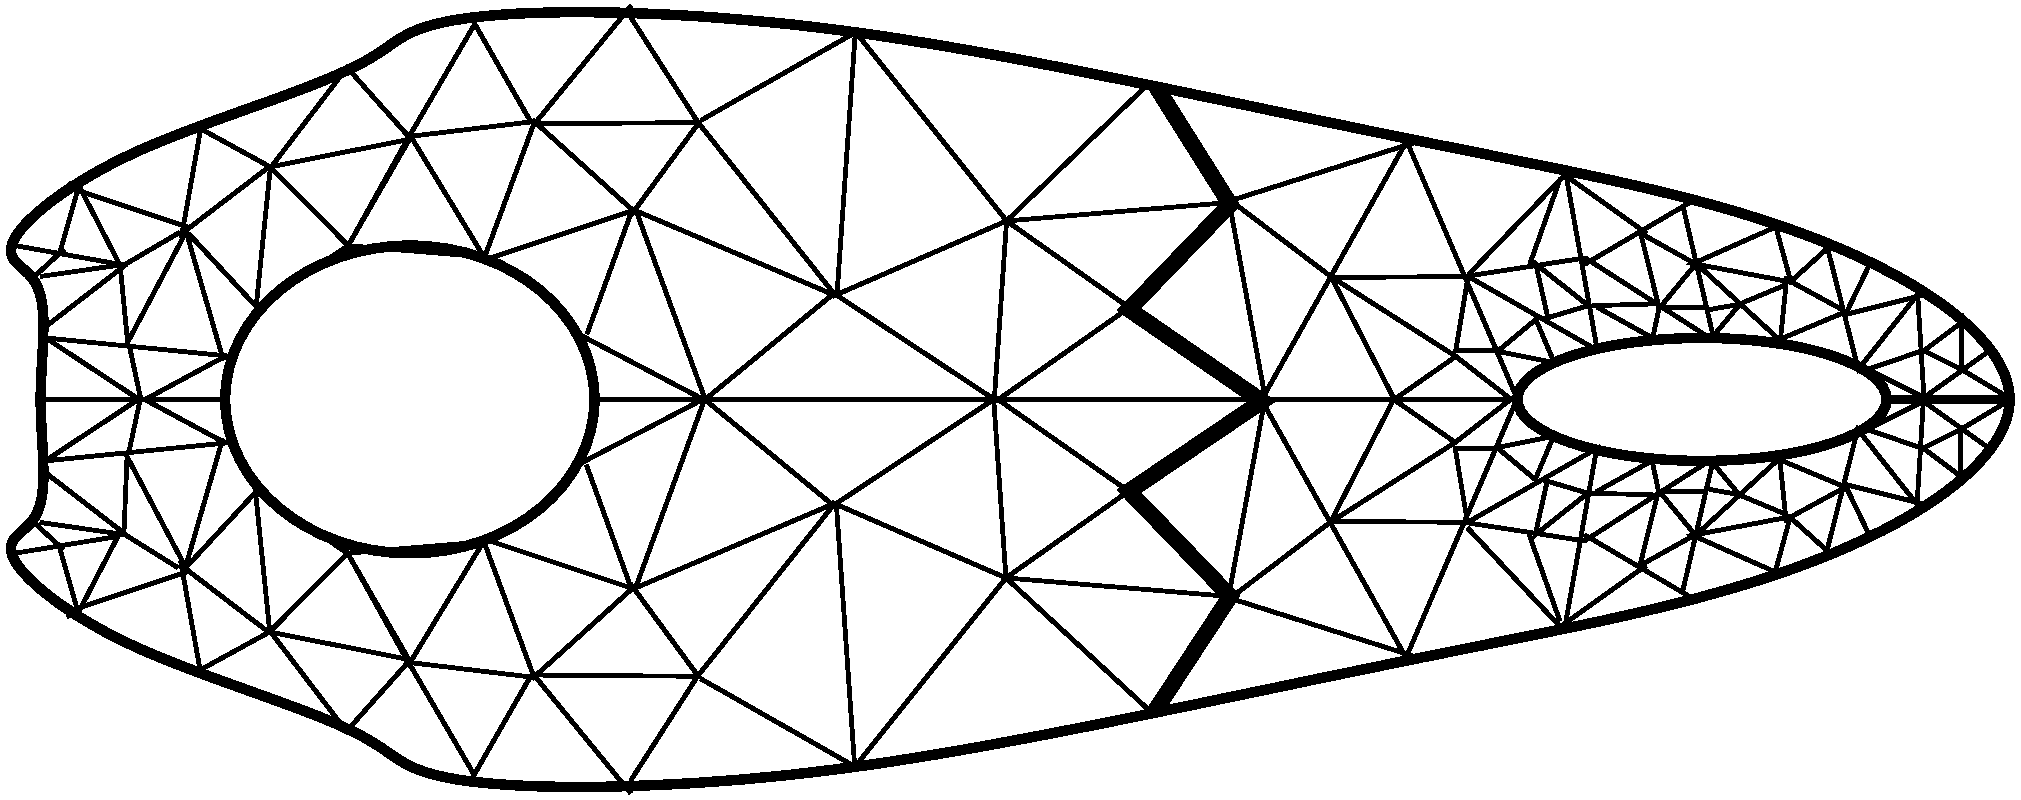
\includegraphics[scale=0.25]{dd_grid}
  \end{center}
  \caption{
    A triangulation of a two-dimensional domains and a partitioning of this
    domain into two subdomains (the bold line represents the subdomain
    interface).
  }
  \label{fig:dd_grid}
\end{figure}

We will not focus on these issues in this course, and stick to simple,
rectangular domains with cartesian meshes.

\subsection{Domain decomposition and parallel computing}

A second important issue related to grid generation is \emph{domain
decomposition}. This is the decompostion of the computational grid into
subdomains, where each subdomain again represents many degrees-of-freedom; see
\autoref{fig:dd_grid}.

Domain decomposition may be important for several reasons. If one is interested
in using a parallel computer with a distributed memory, the global problem
(including the grid) needs to be distributed among the processors. In this
context, each individual subdomain may be associated with a single processor.
However, even on a single process computer, domain decomposition may prove very
useful in the construction of preconditioners for iterative solution methods,
i.e. methods that will speed up the convergence rate when solving the system of
algebraic equations.

Creating a good decomposition from a given grid is not always a trivial task for
general meshes. This is also a field where much progress has been made over the
past few years.

We will come back to this in the course, both in the context of solving the
discretized equation using parallel computers as well as in the context of
preconditioner construction.

\subsection{Adaptivity}

For complex problems, the initial grid is typically generated such that areas
where one expects the solution to exhibit large gradients are well resolved
(i.e. a higher density of elements or degrees-of-freedom is used in those
areas). This approach is very heuristic, and the quality of the underlying mesh
depends strongly on how well one is able to predict the solution structure.

An improved strategy is to use the initial (perhaps coarse) mesh to obtain a
temporary solution which is subsequently used for the purpose of refining the
mesh where the error is expected (or estimated) to be large. This is called
\emph{a posteriori} error estimation and \emph{adaptive} grid refinement (or
perhaps unrefinement). It is an area of considerable research effort since it
promises better error control and reduced computational cost for a fixed error
target. However, adaptive grid refinement is not a trivial task to analyze or to
implement, in particular, for unsteady problems where the solution structure may
change as a function of time.

We will not focus on adaptivity in this course.

\subsection{Visualization}

Once a numerical solution has been computed, the computational results need to
be interpreted. For a multi-dimensional problem, one typically ends up with a
large amount of data. Visualization of these data is often essential in order to
extract useful information from the simulation. Even though the final answer we
are looking for may just be a single number (e.g. the drag), we often want to
understand some of the main features in the solution. With huge amount of data,
visualization (including feature extraction) are invaluable tools. In the
context of parallel computing, visualization is particularly important due to
the very high volume of raw data.

We will consider how to handle the output in this course, but will not focus on
visualization tools. Matlab and Octave will suffice for our needs.

\subsection{Software development}

The effort needed to design and implement a software package for large-scale
simulation of physical systems is typically significant. The associated cost is
therefore also very high. Hence, it is very important to consider good ways to
break down the global problem into smaller modules which can interact in a
flexible and efficient manner.

The use of \emph{object-oriented design} has become popular in recent years. One
of the key issues when designing and implementing a large software package is to
be able to identify commonalities between the various computational tasks, and
to properly encapsulate these so that they may be made into more generic modules
which can be reused for different purposes. An example of this is the solution
of the Poisson equation, which may be used for multiple purposes in the same
simulation package. Another key issue is the concept of data abstraction where
one tries to implement higher-level functionality without necessarily having to
worry about all the details in the lower-level tasks.

\section{Final comments}

It is common to consider the numerical solution of partial differential
equations in the following conceptual model:
\begin{enumerate}
\item we know the computational domain $\Omega$ and the various parameters and
  input data (e.g. the thermal diffusivity $\kappa$ and the volumetric heat
  source $f$);
\item we compute a discrete approximation over the entire domain;
\item we compute the actual output of interest and otherwise interpret and
  visualize the results.
\end{enumerate}

The above approach is often referred to as a \emph{forward problem}, and it may
be sufficient for many problems. However, for certain applications, this mode of
analysis and computation will not suffice. We may not always know the precise
shape of the computational domain, e.g. an airplane wing. In fact, finding the
shape which minimizes the drag may be part of the objective with the simulation.
In such a case, many forward problems are solved, each one hopefully getting
closer to an optimal solution. This type of application represents an example of
an optimization problem. In this context, we note that computing the solution of
a partial differential equation may only give a single data point in a larger
optimization algorithm.

Another area where numerous forward problems may be required is for applications
where the input parameters (e.g. the thermal diffusivity $\kappa$) are not
known, but in fact the quantity of main interest. For such applications, one
will typically have available a certain number of \emph{measurements}
corresponding to multiple \emph{outputs} from the governing equation. The
objective is then to find a distribution of the thermal diffusivity inside the
computational domain such that the difference between the simulated outputs and
the real, physical outputs (or measurements) is minimized. This type of
application represents an example of an \emph{inverse problem}, and is of
significant importance in areas such as medical imaging, estimation of rock
properties etc.


%-------------------------------------------------------------------------------
\newpage
\chapter{Finite differences for Poisson}

\section{Discretization of equations}

When we want to solve a partial differential equation on a computer, we can
typically only do so in an approximate sense, since a computer can only deal
with a finite amount of data. The process of turning a continuous equation into
a finite-dimensional equation suitable for solving on a computer is referred to
as \emph{discretizing} an equation.

There are several ways to go about this, the most popular being \emph{finite
differences}, \emph{finite elements} and \emph{finite volume} discretizations.
Common to all of these approaches is that at the end of the day, the partial
differential equation is turned into a set of linear equations to solve, i.e.
you end up with something on the form
\[
  \bm A \bm u = \bm g
\]
where $\bm A$ is the matrix of linear equations, $\bm u$ is the vector of
unknowns we seek and $\bm g$ is the load (the right hand side in the equation
system).

The simplest and least technical of these are the finite difference approach.
Since this is not a course in numerical solution of partial differential
equations, we will focus on this approach only in this course. But most of what
we consider is also applicable to the other forms of discretization due to the
fact that we will mostly focus on the solution of the linear system of
equations.

\section{Finite difference approximations}

\begin{figure}
  \centering
  \begin{tikzpicture}
  \begin{axis}[
    xmin=-1,
    xmax=1,
    ymin=0,
    ymax=6,
    axis lines=middle,
    axis x line=center,
    hide y axis,
    xtick={-0.7,0.001,0.7},
    xticklabels={$x_i-h$,$x_i$,$x_i+h$},
    xlabel={$x$},
    ]
    \addplot[darkblue, thick, domain=-1:1, samples=100]{x^3+3};
    \draw[thin, densely dashed] (axis cs:0.001,0) -- (axis cs:0,3);
    \draw[thin, densely dashed] (axis cs:-0.7,0) -- (axis cs:-0.7,2.657);
    \draw[thin, densely dashed] (axis cs:0.7,0) -- (axis cs:0.7,3.343);
    \node[shape=circle, draw=darkblue, thick, fill=cadet, inner sep=0.5mm] at (axis cs:-0.7,2.657) {};
    \node[shape=circle, draw=darkblue, thick, fill=cadet, inner sep=0.5mm] at (axis cs:0,3) {};
    \node[shape=circle, draw=darkblue, thick, fill=cadet, inner sep=0.5mm] at (axis cs:0.7,3.343) {};
    \node[anchor=east, xshift=-3mm] at (axis cs:1,4) {$u(x)$};
  \end{axis}
\end{tikzpicture}

  \caption{The function $u(x)$ sampled at a finite difference grid.}
  \label{fig:FiniteDifference}
\end{figure}

Consider the function $u(x)$ depicted in \autoref{fig:FiniteDifference}. A grid
has been introduced---that is, we only consider the function in a discrete sets
of points, $\left\{x_i\right\}_{i=0}^N$, with $x_i = x_0+ih$. Here $h$ is the
grid spacing, here taken as a constant, but in principle we can have a different
spacing between each discrete grid point. We then estimate the derivatives of
this function, only using the values of the function in the discrete sets of
points. This approximation is called a \emph{finite difference}. We now give
alternative finite difference approximations of $u'(x)$ and $u''(x)$ at $x=x_i$.
\begin{align*}
  \intertext{a forward difference approximation:}
  \frac{u(x_i+h)-u(x_i)}{h} &= u'(x_i) + \mathcal{O}(h); \\
  \intertext{two central difference approximations:}
  \frac{u(x_i+h)-u(x_i-h)}{2 h} &= u'(x_i) + \mathcal{O}(h^2), \\ \\
  \frac{u(x_i+h)-2 u(x_i)+u(x_i-h)}{h^2} &= u''(x_i) + \mathcal{O}(h^2).
\end{align*}
The forward difference approximation of $u'(x_i)$ is of first order, meaning
that the error in approximating the first derivative scales linearly with $h$:
if $h$ is reduced by a factor of two, the error is reduced by a factor of two.
The central difference approximations of $u'(x_i)$ and $u''(x_i)$ are of second
order, meaning that the error in approximating the first and second derivatives
scales quadratically with $h$: if $h$ is reduced by a factor of two, the error
is reduced by a factor of four.

We can also generate higher-order approximations to the first and second
derivative of $u(x)$. Higher-order approximations will involve couplings between
more neighboring points.

\section{The one-dimensional Poisson problem}

\subsection{Homogeneous Dirichlet boundary conditions}

We consider here the Poisson equation (or diffusion equation) in one space
dimension,
\begin{align*}
  -u_{xx} = f \qquad \text{in}\,\Omega=(0,1)
\end{align*}
and with homogeneous boundary conditions,
\begin{align*}
  u(0) = u(1) = 0.
\end{align*}

In the following, we will denote the derivative of $u$ with respect to $x$ as
$u_x$, and the second derivative of $u$ with respect to $x$ as $u_{xx}$. This
will prove useful when we later consider two- and three-dimensional problems.

In the Poisson equation, the right hand side $f(x)$ is assumed to be known;
$f(x)$ is often referred to as the source term. In the particular case when
$f=0$, the Poisson equation reduces to the Laplace equation.

In general, the Poisson equation is a partial differential equation (PDE), which
in one space dimension reduces to a standard ordinary differential equation. In
order to obtain a unique solution, we need to specify boundary conditions. In
our case, $u$ is specified at the end points $x=0$ and $x=1$. When $u$ is
specified on the boundary, we say that we have prescribed Dirichlet boundary
conditions. When the prescribed values are zero, as in our case, we say that we
have prescribed homogeneous Dirichlet boundary conditions. The Poisson equation
together with the boundary conditions constitute the Poisson problem.

\begin{figure}
  \centering
  \begin{tikzpicture}
  \begin{axis}[
    xmin=-10,
    xmax=190,
    ymin=0,
    ymax=3,
    axis lines=middle,
    axis x line=center,
    hide y axis,
    xtick={1,180},
    xticklabels={$x=0$, $x=1$},
    ]
    \addplot[darkblue, thick, domain=0:180, samples=100]{sin(x) - 0.4*sin(2*x)};
    \node[anchor=west] at (axis cs:140,1.2) {$u(x)$};
  \end{axis}
\end{tikzpicture}

  \caption{Domain and solution of the one-dimensional Poisson problem.}
  \label{fig:Poisson1D_Domain}
\end{figure}

\begin{figure}
  \centering
  \begin{tikzpicture}
  \draw[thick, darkblue] (0,0) -- (9,0);
  \foreach \i in {0, 1, 5, 9} {
    \draw[thin] (\i,-0.1) -- (\i,0.1);
  }
  \node[anchor=north] at (0,-0.1) {$x_0$};
  \node[anchor=north] at (1,-0.1) {$x_1$};
  \node[anchor=north] at (3,-0.2) {$\cdots$};
  \node[anchor=north] at (5,-0.1) {$x_i$};
  \node[anchor=north] at (7,-0.2) {$\cdots$};
  \node[anchor=north] at (9,-0.1) {$x_N$};
\end{tikzpicture}

  \caption{A finite difference grid.}
  \label{fig:Poisson1D_Grid}
\end{figure}

Let $u_i$ be an approximation to $u(x_i)$, $i=1,\ldots,n-1$, and let $f_i =
f(x_i)$. A finite difference approximation of the Poisson problem can then be
expressed as
\begin{align}
  -\left( \frac{u_{i+1} - 2u_i + u_{i-1}}{h^2} \right) &= f_i, \qquad i=1,\ldots,n-1,
  \label{eq:Poisson_int_1d}\\
  u_0 &= 0, \\
  u_{n} &= 0.
\end{align}
We have here $n-1$ unknown values to determine, namely, $u_1, u_2, \ldots,
u_{n-1}$, and we have $n-1$ conditions by requiring that the Poisson equation be
approximated at all the internal grid points $x_1, x_2, \ldots,x_{n-1}$. The
values $u_0$ and $u_{n}$ follow from satisfying the boundary conditions. Note
that we have here used a second order finite difference approximation of
$u_{xx}$.

The equations (\ref{eq:Poisson_int_1d}) can also be expressed as the system
\begin{align*}
  2 u_1 - u_2 &= h^2 f_1, \\
  -u_1 + 2 u_2 - u_3 &= h^2 f_2, \\
  &\vdots \\
  -u_{n-2} + 2 u_{n-1} &= h^2 f_{n-1}.
\end{align*}
We have here already used the fact that $u_0=0$ and $u_{n}=0$.

In matrix form, this system can be expressed as
\begin{align}
 \underbrace{ \begin{pmatrix}
    2 & -1 & & & \\
    -1 & 2 & -1 & & \\
    & & \ddots & & \\
    & & -1 & 2 & -1 \\
    & & & -1 & 2
  \end{pmatrix}
  }_{\bm A}
  \underbrace{ \begin{pmatrix}
    u_1 \\
    u_2 \\
    \vdots \\
    u_{n-2} \\
    u_{n-1}
  \end{pmatrix}
  }_{\bm u}
  &= h^2
  \underbrace{ \begin{pmatrix}
    f_1 \\
    f_2 \\
    \vdots \\
    f_{n-2} \\
    f_{n-1}
  \end{pmatrix}
  }_{\bm f} ,
  \label{eq:A}
\end{align}
or, more succinctly as
\begin{align*}
  \bm A \bm u = \bm g
\end{align*}
where $\bm g = h^2 \bm f$.

It is common to represent the finite difference formula as a stencil, see
\autoref{fig:ThreePointStencil}. By sweeping this across the grid points on our
mesh, it will generate the linear equations given in \eqref{eq:A}.
\begin{figure}
  \centering
  \begin{tikzpicture}[
  every node/.style={
    shape=circle,
    thick,
    fill=cadet,
    draw=darkblue,
    minimum size=1cm,
  }]
  \draw[thick, darkblue] (-2,0) -- (2,0);
  \node at (-2,0) {$-1$};
  \node at (0,0) {$+2$};
  \node at (2,0) {$-1$};
\end{tikzpicture}

  \caption{
    Weights in the three-point finite difference stencil for the approximation
    of $-h^2u_{xx}$.
  }
  \label{fig:ThreePointStencil}
\end{figure}

We now make some remarks regarding the properties of $\bm A$:
it is a sparse matrix;  more precisely, it is a tridiagonal matrix.
We also note that $\bm A$ is symmetric (i.e., $\bm A = \bm A^\intercal$) and
positive definite (i.e., $\bm v^\intercal \bm A \bm v > 0$ for all vectors $\bm
v \in \mathbb{R}^{n-1}$, $\bm v \not= \bm 0$).

The system of $n-1$ equations is solvable and has a unique solution
\[
  \bm u = \begin{pmatrix} u_1 & u_2 & \cdots & u_{n-1} \end{pmatrix}^\intercal.
\]

The error at the grid points is of second order, i.e.
$|u(x_i)-u_i| \sim \mathcal{O}(h^2)$.

\subsection{Nonhomogeneous Dirichlet boundary conditions}

If $u_0, u_{n} \not= 0$, we can write the $n-1$ equations
\eqref{eq:Poisson_int_1d} as
\begin{align}
  \begin{pmatrix}
    2 & -1 & & & \\
    -1 & 2 & -1 & & \\
    & & \ddots & & \\
    & & -1 & 2 & -1 \\
    & & & -1 & 2
  \end{pmatrix}
  \begin{pmatrix}
    u_1 \\
    u_2 \\
    \vdots \\
    u_{n-2} \\
    u_{n-1}
  \end{pmatrix}
  &= h^2
  \begin{pmatrix}
    f_1 \\
    f_2 \\
    \vdots \\
    f_{n-2} \\
    f_{n-1}
  \end{pmatrix}
  +
  \underbrace{ \begin{pmatrix}
    u_0 \\
    0 \\
    \vdots \\
    0 \\
    u_{n}
  \end{pmatrix}
  }_{\bm b}.
  \label{eq:Poisson1D_DirBC}
\end{align}
This system can again be expressed on the form
\begin{align*}
  \bm A \bm u = \bm g,
\end{align*}
where the left hand side is the same as before. However, the right hand side is
now $\bm g = h^2 \bm f + \bm b$, where the additional vector $\bm b$ is defined
in \eqref{eq:Poisson1D_DirBC}.

\section{Two-dimensional Poisson problem}

We now consider the Poisson problem in a rectangular domain with lengths $L_x$
and $L_y$; see \autoref{fig:Poisson2D_Domain}. The Poisson problem we consider
can be expressed as
\begin{alignat*}{2}
  -\nabla^2 u &= f & \qquad &\text{in}\, \Omega, \\
  u &= 0 & \qquad & \text{on}\, \partial \Omega.
\end{alignat*}
where the right hand side $f(x,y)$ (the source term) is assumed to be known.

\begin{figure}
  \centering
  \begin{tikzpicture}
    \begin{axis}[
      width=8cm,
      height=6cm,
      scale=0.8,
      xmin=0, xmax=4,
      ymin=0, ymax=3,
      axis lines=middle,
      ticks=none,
      xlabel=$x$,
      ylabel=$y$,
      ]
      \draw[darkblue, fill=cadet] (axis cs:0,0) rectangle (axis cs:3,2);
      \node[anchor=south] at (axis cs:3,2) {$(L_x,L_y)$};
      \node at (axis cs:1.5,1) {$\Omega$};
    \end{axis}
  \end{tikzpicture}
  \caption{A rectangular domain for the two-dimensional Poisson problem.}
  \label{fig:Poisson2D_Domain}
\end{figure}

\begin{figure}
  \centering
  \begin{tikzpicture}[scale=0.5]
  \foreach \i in {0,2,4,6,8,10} {
    \draw[thick, darkblue] (\i,0) -- (\i,8);
  }
  \foreach \j in {0,2,4,6,8} {
    \draw[thick, darkblue] (0,\j) -- (10,\j);
  }
  \draw[thick, darkblue, fill=cadet] (4,4) circle (2mm);
  \node[anchor=east] at (0,0) {$y_0$};
  \node[anchor=east] at (0,4) {$y_j$};
  \node[anchor=east] at (0,8) {$y_m$};
  \node[anchor=north] at (0,0) {$x_0$};
  \node[anchor=north] at (4,0) {$x_i$};
  \node[anchor=north] at (10,0) {$x_n$};
\end{tikzpicture}

  \caption{Finite difference grid: a structured grid.}
  \label{fig:Poisson2D_Grid}
\end{figure}

\subsection{Finite difference discretization}

The finite difference grid points (or nodes) in \autoref{fig:Poisson2D_Grid} are
given by
\begin{align*}
  x_i &= i \cdot h_x, \quad i=0,1,\ldots,m, \qquad h_x = \frac{L_x}{m}, \\
  y_j &= j \cdot h_y, \quad j=0,1,\ldots,n, \qquad h_y = \frac{L_y}{n}.
\end{align*}
Let $u_{i,j}$ be an approximation to $u(x_i,y_j)$, $1\leq i\leq m-1$, $1\leq
j\leq n-1$, and let $f_{i,j} = f(x_i,y_j)$. Then
\begin{align*}
  \frac{u_{i+1,j} - 2 u_{i,j} + u_{i-1,j}}{h_x^2}
  &\simeq \left( \frac{\partial^2 u}{\partial x^2} \right) \biggl|_{(x_i,y_j)} + \mathcal{O}(h_x^2), \\
  \frac{u_{i,j+1} - 2 u_{i,j} + u_{i,j-1}}{h_y^2}
  &\simeq \left( \frac{\partial^2 u}{\partial y^2} \right) \biggl|_{(x_i,y_j)} + \mathcal{O}(h_y^2).
\end{align*}

Assuming (for simplicity) that $m=n$, and that $h_x=h_y=h$, the approximation of
the Poisson problem at the internal grid points can be expressed as
\begin{align*}
  -\frac{(u_{i+1,j}-2u_{i,j}+u_{i-1,j})}{h^2}
  -\frac{(u_{i,j+1}-2u_{i,j}+u_{i,j-1})}{h^2}
  &= f_{i,j}, \qquad i,j=1,\ldots,n-1,
\end{align*}
or
\begin{align}
  -u_{i+1,j}-u_{i-1,j}-u_{i,j+1}-u_{i,j-1}+4u_{i,j} &= h^2 f_{i,j}, \qquad i,j=1,\ldots,n-1.
  \label{eq:Poisson2D_disc}
\end{align}
We note that each unknown value $u_{i,j}$ is coupled to its nearest neighbors
(north, south, east, west) according to the five-point stencil we are using; see
\autoref{fig:FivePointStencil}.

\begin{figure}
  \centering
  \begin{tikzpicture}[
  every node/.style={
    shape=circle,
    thick,
    fill=cadet,
    draw=darkblue,
    minimum size=1cm,
  }]
  \draw[thick, darkblue] (-2,0) -- (2,0);
  \draw[thick, darkblue] (0,-2) -- (0,2);
  \node at (-2,0) {$-1$};
  \node at (2,0) {$-1$};
  \node at (0,-2) {$-1$};
  \node at (0,2) {$-1$};
  \node at (0,0) {$+4$};
\end{tikzpicture}

  \caption{
    Weights in the five-point finite difference stencil for the approximation of
    $-h^2\nabla^2$.
  }
  \label{fig:FivePointStencil}
\end{figure}

\subsection{Global numbering scheme}

In order to generate a matrix system as in the one-dimensional case, we need to
define a unique ordering of all the degrees-of-freedom. We will here use a
``natural'' ordering in the sense that we number the \emph{internal} nodes along
the $x$-direction first, i.e.
\begin{align*}
  u_{k=(n-1)(j-1)+i} & \equiv u_{i,j} \\
  f_{k=(n-1)(j-1)+i} &\equiv f_{i,j}
\end{align*}
Here, $k = 1,\ldots,N$ with $N=(n-1)^2$. We see that the ordering maps each
node, $(i,j)$, in the grid to a unique, global index, $k$; see
\autoref{fig:NaturalOrdering}.

\begin{figure}
  \centering
  \begin{tikzpicture}[
  block/.style={
    shape=circle,
    thick,
    draw=darkblue,
    fill=cadet,
    inner sep=0.2mm,
    minimum size=8mm,
  }]
  \node[block] at (0,0) {\tiny $1$};
  \node[block] at (1,0) {\tiny $2$};
  \node[block] at (2,0) {\tiny $3$};
  \node[block] at (3,0) {\tiny $4$};
  \node at (4,0) {\ldots};
  \node[block] at (5,0) {\tiny $n$};

  \node[block] at (0,1) {\tiny $n+1$};
  \node[block] at (1,1) {\tiny $n+2$};
  \node[block] at (2,1) {\tiny $n+3$};
  \node[block] at (3,1) {\tiny $n+4$};
  \node at (4,1) {\ldots};
  \node[block] at (5,1) {\tiny $2n$};

  \node[yshift=1mm] at (5,2) {$\vdots$};
  \node[block] at (5,3) {\tiny $mn$};

  \node at (0,-0.7) {\tiny $i=1$};
  \node at (1,-0.7) {\tiny $i=2$};
  \node at (2,-0.7) {\tiny $i=3$};
  \node at (3,-0.7) {\tiny $i=4$};
  \node at (5,-0.7) {\tiny $i=n$};
  \node at (-0.9,-0.05) {\tiny $j=1$};
  \node at (-0.9,0.95) {\tiny $j=2$};
  \node at (-0.9,2.95) {\tiny $j=m$};
\end{tikzpicture}

  \caption{
    We use a ``natural'' ordering of the unknowns: we first number all the
    \emph{internal} nodes along ``row'' 1 (in the $x$-direction), followed by
    the nodes in ``row'' 2, etc. The boundary nodes are not counted since these
    values are assumed to be known.
  }
  \label{fig:NaturalOrdering}
\end{figure}

\subsection{System of equations}

With the chosen numbering scheme of the unknowns, we can express the discrete
equations \autoref{eq:Poisson2D_disc} as
\begin{equation}
  \underbrace{
    \begin{pmatrix}
      \bm A_0 & \bm A_1 & & & \\
      \bm A_1 & \bm A_0 & \bm A_1 & & \\
      & \bm A_1 & \bm A_0 & \ddots & \\
      & & \ddots & \ddots & \bm A_1 \\
      & & & \bm A_1 & \bm A_0
    \end{pmatrix}}_{\bm A}
  \underbrace{
    \begin{pmatrix}
      u_1 \\ u_2 \\ u_3 \\ \vdots \\ u_N
    \end{pmatrix}}_{\bm u}
  =
  \underbrace{
    \begin{pmatrix}
      f_1 \\ f_2 \\ f_3 \\ \vdots \\ f_N
    \end{pmatrix}}_{\bm g}
  \label{eq:Poisson2D_sys}
\end{equation}
where the matrices $\bm A_0$ and $\bm A_1$ are defined as
\begin{equation}
  \bm A_0 =
  \begin{pmatrix}
    4 & -1 & & & \\
    -1 & 4 & -1 & & \\
    & -1 & 4 & \ddots & \\
    & & \ddots & \ddots & -1 \\
    & & & -1 & 4
  \end{pmatrix}
  \qquad
  \bm A_1 =
  \begin{pmatrix}
    -1 & & & & \\
    & -1 & & & \\
    & & -1 & & \\
    & & & \ddots & \\
    & & & & -1
  \end{pmatrix}.
\end{equation}
The dimension of this system is $N=(n-1)^2$. The matrix $\bm A$ is still sparse;
in particular, it is pentadiagonal, reflecting the use of a five-point stencil
for the approximation of the Laplace operator. However, while the bandwidth in
the one-dimensional case is one, the bandwidth is now $n$.

Finally, we remark that the matrix $\bm A$ is symmetric and positive definite as
in the one-dimensional case. This will guarantee that the system
\eqref{eq:Poisson2D_sys} is solvable and will yield a unique solution
$\bm u = \begin{pmatrix}u_1&\cdots&u_N\end{pmatrix}^\intercal$. The
discretization error is still quadratic in the grid spacing $h$,
\begin{align*}
  |u(x_i,y_j)-u_{i,j}| \sim \mathcal{O}(h^2). \\
\end{align*}

\subsection{Solution methods for $\bm A \bm u = \bm g$}

Once we have generated the system of equations $\bm A \bm u = \bm g$, we need to
solve this system. There are two main classes of solution methods: direct and
iterative methods. We now give a brief discussion of each of these classes.

\subsubsection{Direct methods}

A direct solution method is method which solves the system of algebraic
equations in a finite, predictable number of steps, e.g., Gaussian elimination,
FFT, etc. This class of the solution methods is often robust, especially when
$\bm A$ is symmetric and positive definite.

In the following, we will use the following notation:
\begin{align*}
  \mathcal{N}_\text{op} &= \text{number of floating-point operations} \\
  \mathcal{M} &= \text{memory requirement (in number of bytes)}
\end{align*}

We will also assume that $\bm A \in \mathbb{R}^{N \times N}$.

As an example, consider full LU-factorization (Gaussian elimination). In this
case, we do not exploit any information about sparsity of $\bm A$, but treat
this as a full matrix. For this solution approach, we have
\begin{align*}
  \mathcal{N}_\text{op} &\sim \mathcal{O}(N^3), \\
  \mathcal{M} &\sim \mathcal{O}(N^2).
\end{align*}
Full LU-factorization is robust and easy to use, however the cost does not scale
very well since we need $\mathcal{O}(N^2)$ operations per unknown. For large
systems, this cost becomes prohibitive.

A better approach is to exploit the banded structure of $\bm A$. For a banded
LU-factorization of bandwidth $b$, we have
\begin{align*}
  \mathcal{N}_\text{op} &\sim \mathcal{O}(N b^2) ,\\
  \mathcal{M} &\sim \mathcal{O}(N b) .
\end{align*}

We remark that, since $\bm A$ is symmetric and positive definite, no pivoting is
necessary during the Gaussian elimination process.

\begin{figure}
  \centering
  \begin{tikzpicture}
    \foreach \i in {0,...,4} {
      \draw[darkblue, very thick] (0,\i) -- (4,\i);
      \draw[darkblue, very thick] (\i,0) -- (\i,4);
    }
    \node[anchor=east] at (0,2) {$n$};
    \node[anchor=north] at (2,0) {$n$};
  \end{tikzpicture}
  \caption{
    The two-dimensional grid associated with the finite difference solution of
    the Poisson problem. Here, $N \sim n^2$, while the bandwidth of
    $\bm A$ using a natural numbering scheme is $b\sim n$.
  }
  \label{fig:Poisson_nxn}
\end{figure}

Let us now revisit \eqref{eq:Poisson2D_sys} which we arrived at based on a
finite difference discretization of the two-dimensional Poisson problem. If we
exploit the banded structure of $\bm A$ during the LU-factorization, see
\autoref{fig:Poisson_nxn}, the cost of this method is
\begin{align*}
  \mathcal{N}_\text{op} &\sim \mathcal{O}(N b^2)
                          \sim \mathcal{O}(n^4) \sim \mathcal{O}(N^2)\\
  \mathcal{M} &\sim \mathcal{O}(N b) \sim \mathcal{O}(n^3) \sim \mathcal{O}(N^{3/2})
\end{align*}

However, if we instead use FFT (The Fast Fourier Transform), as we will discuss
later, the cost of solving \eqref{eq:Poisson2D_sys} is only
\begin{align*}
  \mathcal{N}_{op} &\sim \mathcal{O}(N \log N), \\
  \mathcal{M} &\sim \mathcal{O}(N).
\end{align*}
This is approximately optimal since the computational cost is $\mathcal{O}(\log
N)$ per unknown, and the memory requirement is constant per unknown, independent
of the value of $N$.

\subsubsection{Iterative methods}

An iterative method will give a new estimate or update of the solution at each
iteration. In most cases, the exact solution to $\bm A \bm u = \bm g$ will never
be reached. However, one can get as close as one wishes, but this may require
many iterations and imply a high computational cost. Unlike a direct method, the
solution is not reached after a finite, predictable number of floating point
operations. In order to stop the iteration, a stop criterion has to be specified
by the user. This can be some kind of tolerance, e.g. that the residual (i.e.
the difference between the left hand side and the right hand side of the
equation system) is less than a tolerance. Typically, when the tolerance is
reduced, the number of iterations increases.

Another aspect with iterative methods is that the computational cost can be
problem dependent; see \autoref{fig:Poisson_aspect}. This is different from
direct solution methods which often only depends on the problem size, $N$.

\begin{figure}
  \centering
  \begin{tikzpicture}
    \foreach \i in {0,...,4} {
      \draw[darkblue, very thick] (-2,\i) -- (2,\i);
      \draw[darkblue, very thick] (-2+\i,0) -- (-2+\i,4);
      \draw[darkblue, very thick] (-6,-5+\i) -- (6,-5+\i);
      \draw[darkblue, very thick] (-6+3*\i,-5) -- (-6+3*\i,-1);
    }
  \end{tikzpicture}
  \caption{
    Two different computational domains for the Poisson problem, but with the
    same number of unknowns after discretization. The problem size, $N$, is
    therefore the same. The number of iterations required to solve the system of
    algebraic equations will depend on the aspect ratio (the ratio $L_x/L_y$) of
    the domains. Hence, the computational cost for solving the problem on the
    right will be higher than for the problem on the left. This is in contrast
    to a direct method where the computational cost for solving the two systems
    will be the same.
  }
  \label{fig:Poisson_aspect}
\end{figure}

A great advantage of many iterative methods is that they often have a
\emph{scalable} memory requirement, i.e. that the memory requirement is
proportional to $N$ and not some power of $N$.

Another characteristics with iterative methods is that much of the computational
cost is related to performing basic linear algebra operations such as
matrix-vector products, inner products, etc.

Finally, we remark that iterative methods are very suitable for parallel
processing, and are often the only viable alternative for large,
three-dimensional problems.

Some examples of iterations methods suitable for symmetric and positive definite
problems are: Jacobi iteration, Gauss-Seidel iteration, the conjugate gradient
method, and multigrid methods (where the last two methods are commonly used
today).


%-------------------------------------------------------------------------------
\newpage
\chapter{Diagonalization for Poisson}

\section{Direct method based on diagonalization}

Let us now consider a different way of solving the finite difference equations
we derived in the context of discretizing the Poisson problem. The method is
based on \emph{diagonalization}, and we first explain the approach in the context
of the one-dimensional Poisson problem:

\begin{align*}
  -u_{xx} &= f \quad \text{in}\, \Omega = (0,1), \\
  u(0) = u(1) &= 0.
\end{align*}
Assume that we use a uniform finite difference grid given by:
\begin{equation*}
  x_i = x_0 + ih, \quad i=0,1,\ldots,n.
\end{equation*}

The corresponding system of algebraic equations can be written as
\begin{align*}
  \frac{1}{h^2}
  \begin{pmatrix}
    2 & -1 & & & \\
    -1 & 2 & -1 & & \\
    & -1 & 2 & -1 & \\
    & & & \ddots & -1 \\
    & & & -1 & 2
  \end{pmatrix}
  \begin{pmatrix}
    u_1 \\
    u_2 \\
    \vdots \\
    u_{n-1}
  \end{pmatrix}
  =
  \begin{pmatrix}
    f_1 \\
    f_2 \\
    \vdots \\
    f_{n-1}
  \end{pmatrix},
\end{align*}
where $u_i$ is an approximation to $u(x_i) = u(ih),$ $i=1,\ldots,n-1$,
$f_i=f(x_i)$, and $u_0 = u_n = 0$ due to the specified boundary conditions. Let us write this system as

\begin{align*}
  \frac{1}{h^2} \matT \uu = \bff
\end{align*}
where
\begin{align*}
  \matT =
  \begin{pmatrix}
    2 & -1 & & & \\
    -1 & 2 & -1 & & \\
    & -1 & 2 & -1 & \\
    & & & \ddots & -1 \\
    & & & -1 & 2
  \end{pmatrix} , \qquad
  \uu =
  \begin{pmatrix}
    u_1 \\
    \vdots \\
    u_{n-1}
  \end{pmatrix} , \qquad
  \bff =
  \begin{pmatrix}
    f_1 \\
    \vdots \\
    f_{n-1}
  \end{pmatrix},
\end{align*}
and $h$ is the grid size or mesh size. Since $\matT$ is symmetric
positive definite, it can be \emph{diagonalized}.

\subsection{Diagonalization of $\matT$}

Diagonalization of $\matT$ means that we wish to find the eigenvalues
$\lambda_j$ and the eigenvectors $\matQ_j$ of $\matT$,
\begin{align*}
  \matT \matQ_j &= \lambda_j \matQ_j \quad j=1,\ldots,n-1,
\end{align*}
where
\begin{align*}
  \lambda_j &> 0 \qquad &\text{(positive eigenvalues)}, \\
  \matQ_k^\intercal \matQ_j &= \delta_{jk} \qquad &\text{(orthonormal eigenvectors)}.
\end{align*}

We collect all the eigenvectors $\matQ_j$ into the orthogonal matrix $\matQ$,
\begin{equation*}
  \matQ = \begin{pmatrix} \matQ_1 & \matQ_2 & \cdots & \matQ_{n-1}\end{pmatrix}.
\end{equation*}
Then
\begin{align*}
  \matT \matQ &= \matQ \bm \Lambda
\end{align*}
where
\begin{align*}
  \bm \Lambda &= \operatorname{diag}(\lambda_1, \ldots, \lambda_{n-1}) =
  \begin{pmatrix}
    \lambda_1 & & \\
     & \ddots & \\
    & & \lambda_{n-1}
  \end{pmatrix}.
\end{align*}
Since
\begin{align*}
  \matQ^\intercal \matQ = \bm I =
  \begin{pmatrix}
    1 & & \\
    & \ddots & \\
    & & 1
  \end{pmatrix} \qquad
  \Rightarrow \quad \matQ^\intercal = \matQ^{-1},
\end{align*}
and
\begin{align}
  \matT &= \matQ \bm \Lambda \matQ^\intercal
  \label{eq:T_diag}
\end{align}
or
\begin{align*}
  \matQ^\intercal \matT \matQ = \bm \Lambda \qquad \text{(diagonal)}.
\end{align*}

Following this approach the finite difference approximation can be computed as
follows:
\begin{alignat*}{2}
  \bm g &\equiv  h^2 \bff \quad &  \qquad \qquad \bm g
  &: \; \mathcal{O}(n) ~ \text{operations} \\
  \\
  \matT \, \uu &= \bm g \\
  \matQ \, \bm \Lambda \, \matQ^\intercal \uu &= \bm g \\
  \bm \Lambda \underbrace{\matQ^\intercal \uu}_{\tilde{\uu}}
  &= \underbrace{\matQ^\intercal \bm g}_{\tilde{\bm g}}
  & \tilde{\bm g} &: \; \mathcal{O}(n^2) ~ \text{operations} \\
  \\
  \bm \Lambda \tilde{\uu} &= \tilde{\bm g} \\
  \tilde{\uu} &= \bm \Lambda^{-1} \tilde{\bm g}
  & \tilde{\uu} &: \; \mathcal{O}(n) ~ \text{operations} \\
  \\
  \matQ^\intercal \uu &= \tilde{\uu} \\
  \uu &= \matQ \tilde{\uu} & \uu
  &: \; \mathcal{O}(n^2) ~ \text{operations}
\end{alignat*}
Note that the transformations
\begin{equation*}
  \tilde{\bm g} = \matQ^\intercal \bm g \quad \text{and} \quad \uu = \matQ \tilde{\uu}
\end{equation*}
are \emph{matrix-vector products}. In summary, we can compute $\uu$ in
\begin{equation*}
  \mathcal{O}(n) + \mathcal{O}(n^2) + \mathcal{O}(n) + \mathcal{O}(n^2)
  \sim \mathcal{O}(n^2) ~ \text{floating-point operations}.
\end{equation*}
Hence, we can solve our finite difference system in $(n-1)$ unknowns in
$\mathcal{O}(n^2)$ operations. This is \emph{not} competitive with a direct
solution algorithm based upon LU-factorization (Gaussian elimination) of a
tridiagonal matrix, which can be done in $\mathcal{O}(n)$ operations (since the
bandwidth is equal to one).

Let us also compare the memory requirement:
\begin{align*}
  &\mathcal{O}(n^2) ~\text{for the diagonalization approach
  (we need to store $\matQ$)}; \\
  &\mathcal{O}(n) ~\text{for a tridiagonal direct solver}.
\end{align*}
Again, the diagonalization approach is {\em not} competitive.

So, why bother? The answer is that the diagonalization approach becomes more
interesting in $\mathbb{R}^2$. In addition, we will later see how we can use the
Fast Fourier Transform (FFT) to lower the computational complexity.

\section{The Poisson problem in $\mathbb{R}^2$}

The two-dimensional Poisson problem on the unit square is given by

\begin{equation}
  \begin{split}
    -\nabla^2 u &= f \qquad \text{in} ~ \Omega=(0,1) \times (0,1), \\
    u &= 0 \qquad \text{on} ~ \partial \Omega, \\
  \end{split}
  \label{eq:Poisson2D}
\end{equation}
where
\[
  \nabla^2 u = \frac{\partial^2 u}{\partial x^2}
  + \frac{\partial^2 u}{\partial y^2}.
\]

%XXX
%\begin{figure}
%  \centering
%  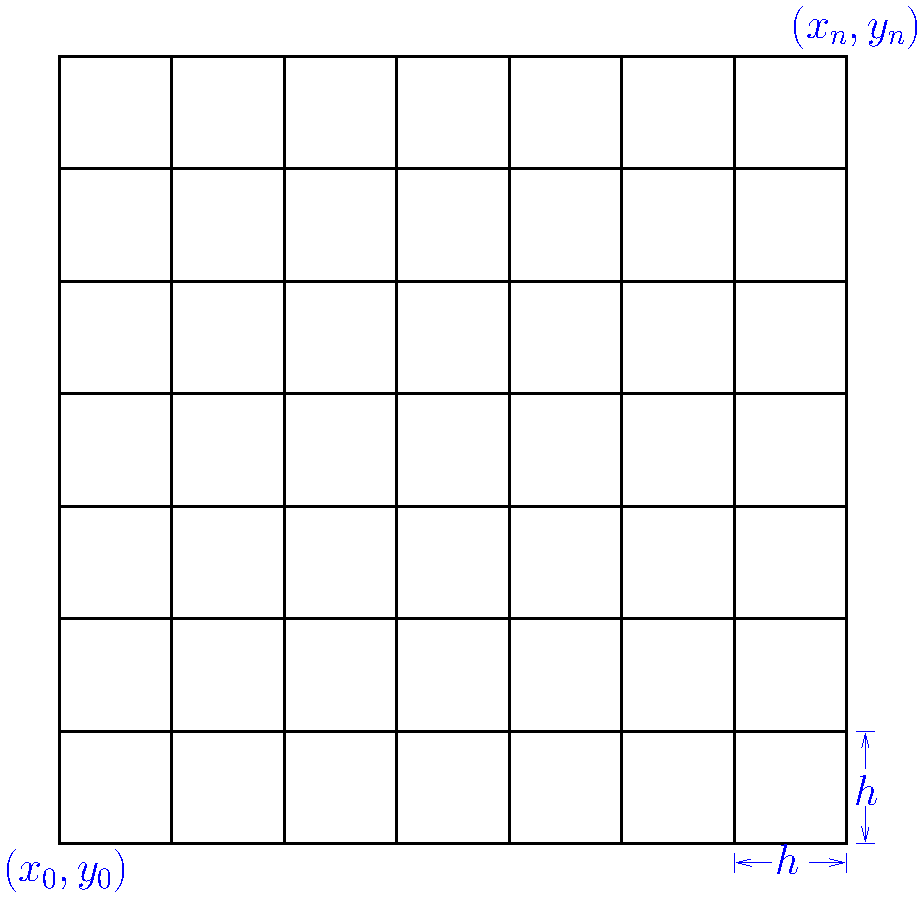
\includegraphics[width=8cm]{FiniteDifferenceGrid}
%    \caption{A uniform finite difference grid.}
%  \label{fig:FDM_grid_2D}
%\end{figure}

Again, using the notation $u_{i,j} \simeq u(x_i,y_j) = u(i h, j h)$ and
$f_{i,j}=f(x_i,y_j)$, and discretizing \eqref{eq:Poisson2D} using the 5-point
stencil (see Figure \ref{fig:FDM_grid_2D}), the discrete equations read
\begin{equation}
  -\frac{(u_{i+1,j}-2u_{i,j}+u_{i-1,j})}{h^2} - \frac{(u_{i,j+1}-2u_{i,j}+u_{i,j-1})}{h^2} = f_{i,j}
  \label{eq:FDM_sys}
\end{equation}
for $1 \leq i,j \leq n-1$.

\subsection{Diagonalization}

Let
\begin{equation*}
  \uu =
  \begin{pmatrix}
    u_{1,1} & \cdots & u_{1,n-1} \\
    \vdots & \ddots & \vdots \\
    u_{n-1,1} & \cdots & u_{n-1,n-1}
  \end{pmatrix}
\end{equation*}
and
\begin{equation*}
  \matT =
  \begin{pmatrix}
    2 & -1 & & & \\
    -1 & 2 & -1 & & \\
    & & \ddots & & \\
    & & -1 & 2 & -1 \\
    & & & -1 & 2
  \end{pmatrix}.
\end{equation*}

Then,
\begin{alignat*}{2}
  (\matT \uu)_{ij} &= 2u_{i,j} - u_{i+1,j}, & \qquad i=1, \\
  (\matT \uu)_{ij} &= -u_{i-1,j}+2u_{i,j} - u_{i+1,j}, &\qquad 2 \leq i \leq n-2, \\
  (\matT \uu)_{ij} &= -u_{i-1,j}+2u_{i,j}, &\qquad i=n-1.
\end{alignat*}
and thus,
\begin{equation}
  \frac{1}{h^2} (\matT \uu)_{ij} \simeq
  - \left( \frac{\partial^2 u}{\partial x^2} \right)_{i,j}.
\end{equation}

Similarly in the other direction,
\begin{equation}
  \frac{1}{h^2} (\uu \matT)_{ij} \simeq
  - \left( \frac{\partial^2 u}{\partial y^2} \right)_{i,j}.
\end{equation}

Our finite difference system (\ref{eq:FDM_sys}) can thus be expressed as
\begin{equation*}
  \frac{1}{h^2} (\matT \uu + \uu \matT)_{ij} = f_{i,j}
  \qquad \text{for} \qquad 1 \leq i,j \leq n-1, \\
\end{equation*}
or
\begin{equation}
  \matT \uu + \uu \matT = \bm G
  \label{eq:Poisson2D_TUUT}
\end{equation}
where
\begin{equation*}
  \bm G = h^2
  \begin{pmatrix}
    f_{1,1} & \ldots & f_{1,n-1} \\
    \vdots & \ddots & \vdots \\
    f_{n-1,1} & \ldots & f_{n-1,n-1}
  \end{pmatrix}.
\end{equation*}

Combining \eqref{eq:T_diag} and \eqref{eq:Poisson2D_TUUT} we get
\begin{equation}
  \matQ \bm \Lambda \matQ^\intercal \uu + \uu \matQ \bm \Lambda \matQ^\intercal = \bm {G}.
  \label{eq:Poisson2D_T_diag}
\end{equation}

Multiplying \eqref{eq:Poisson2D_T_diag} from the right with $\matQ$ and from the
left with $\matQ^\intercal$, and using the fact that $\matQ^\intercal \matQ =
\bm I$, we get
\begin{equation*}
  \bm \Lambda \underbrace{\matQ^\intercal \uu \matQ}_{\tilde{\uu}} +
  \underbrace{\matQ^\intercal \uu \matQ}_{\tilde{\uu}} \bm \Lambda =
  \underbrace{\matQ^\intercal \bm G \matQ}_{\tilde{\bm G}}.
\end{equation*}

Hence, (\ref{eq:Poisson2D_TUUT}) may be solved in three steps:

\begin{enumerate}
\item Compute $\tilde{\bm G}$ using matrix-matrix products
  \begin{equation*}
    \tilde{\bm G} = \matQ^\intercal \bm G \matQ.
  \end{equation*}
\item Solve for $\tilde{\uu}$.
  \begin{align*}
    \bm \Lambda \tilde{\uu} + \tilde{\uu} \bm \Lambda &= \tilde{\bm G} \\
    \lambda_i \tilde{u}_{ij} + \tilde{u}_{ij} \lambda_j &= \tilde{g}_{ij} \\
    \tilde{u}_{ij} &= \frac{\tilde{g}_{ij}}{\lambda_i + \lambda_j}
  \end{align*}
\item Compute $\uu$ using matrix-matrix products
  \begin{equation*}
    \uu = \matQ \tilde{\uu} \matQ^\intercal
  \end{equation*}
\end{enumerate}

Here,
\begin{equation*}
  \uu, \tilde{\uu}, \tilde{\bm G}, \matQ \in \mathbb{R}^{(n-1) \times (n-1)}
\end{equation*}

\subsubsection{Computational cost}

The number of degrees of freedom (or unknowns) $N$ is
\begin{align*}
N = (n-1)^2 \sim \mathcal{O}(n^2) \quad (n \gg 1).\\
\end{align*}

\begin{enumerate}
\item Two matrix-matrix products give $\mathcal{O}(n^3)$ operations.
\item $\mathcal{O}(n^2)$ scalar constant time operations give $\mathcal{O}(n^2)$.
\item Two matrix-matrix products give $\mathcal{O}(n^3)$ operations.
\end{enumerate}
In summary, we can compute the discrete solution, $\uu$, in
$\mathcal{O}(n^3)=\mathcal{O}(N^{3/2})$ operations.

Note: this method is an example of a {\em direct method}.

\subsubsection{Comparison with other direct methods}

\begin{table}
    \caption{
      Computational cost and memory requirement for three different
      direct methods. The number of unknowns is $N=\mathcal{O}(n^2)$. For the
      banded solver, we have used a bandwidth $b \sim \mathcal{O}(n)$. Full LU
      means LU-factorization without exploiting sparsity.
    }
    \label{tab:DirectMethods_ComputationalCost}
  \begin{center}
    \bgroup\def\arraystretch{1.2}
    \begin{tabular}{lrr}
      \hline
      Method & Operations ($\mathcal{N}_\text{op}$) & Memory requirement ($\mathcal{M}$) \\
      \hline
      Diagonalization & $\mathcal{O}(N^{3/2}) = \mathcal{O}(n^3)$ & $\mathcal{O}(N) = \mathcal{O}(n^2)$ \\
      Banded LU & $\mathcal{O}(N b^2) = \mathcal{O}(n^4)$ & $\mathcal{O}(Nb) = \mathcal{O}(n^3)$ \\
      Full LU & $\mathcal{O}(N^3) = \mathcal{O}(n^6)$ & $\mathcal{O}(N^2) = \mathcal{O}(n^4)$ \\
      \hline
    \end{tabular}
    \egroup
  \end{center}
\end{table}

We conclude that the diagonalization method is much more attractive in
$\mathbb{R}^2$ than in $\mathbb{R}^1$. The number of floating-point operations
per degree of freedom is $\mathcal{O}(n)$, while the memory requirement is close to optimal (i.e. scalable).

\subsubsection{The matrices $\matQ$ and $\bm \Lambda$}

The computational cost associated with the diagonalization approach tacitly
assumes that we know the eigenvector matrix $\matQ$ and the corresponding
eigenvalues. Let us therefore derive explicit expressions for these. To this
end, consider first the continuous eigenvalue problem
\begin{equation*}
  \begin{split}
    -u_{xx} &= \lambda u \qquad \qquad \text{in } \Omega=(0,1), \\
    u(0) = u(1) &= 0,
  \end{split}
\end{equation*}
with solutions
\begin{equation*}
  \begin{split}
    \bar{u}_j(x) &= \sin(j \pi x), \\
    \bar{\lambda}_j &= j^2 \pi^2,
  \end{split}
  \qquad j=1,2,\ldots,\infty.
\end{equation*}

Consider now the discrete eigenvalue problem
\begin{equation*}
  \matT \tilde{\matQ}_j =
  \lambda_j \tilde{\matQ}_j
\end{equation*}
Try eigenvector solutions which correspond to the continuous eigenfunctions
$\bar{u}_j(x)$ sampled at the grid points $x_i, i=1,\ldots,n-1$, i.e.
\begin{equation*}
  \begin{split}
    (\tilde{\matQ}_j)_i &= \bar{u}_j (x_i) \\
    &= \sin(j \pi x_i) \\
    &= \sin(j \pi (i h)), \\
    &= \sin \left(\frac{i j \pi}{n} \right)
  \end{split}
\end{equation*}

Operating on $\tilde{\matQ}_j$ with $\matT$ gives
\begin{equation*}
  (\matT \tilde{\matQ}_j)_i =
  \underbrace{2\left( 1 - \cos\left( \frac{j\pi}{n} \right) \right)}_{\lambda_j}
  \underbrace{\sin\left( \frac{i j \pi}{n} \right)}_{(\tilde{\matQ}_j)_i}
\end{equation*}

Hence, our try was successful: operating on $\tilde{\matQ}_j$ with $\matT$ gives
a multiple of $\tilde{\matQ}_j$.

In order to proceed, set $\matQ_j = \alpha \tilde{\matQ}_j$, and choose $\alpha$
such that $\matQ_j$ is normalized:

\begin{align*}
  (\matQ_j)_i &= \sqrt{\frac{2}{n}} \sin \left( \frac{ij \pi}{n} \right),
                \qquad \qquad 1 \leq i,j \leq n-1, \\
  \lambda_j &= 2 \left( 1 - \cos \left( \frac{j \pi}{n} \right) \right).
\end{align*}

For ${j \ll n}$, we observe that
\begin{align*}
  \lambda_j
  &\simeq 2 \left( 1 - \left( 1 -\frac{1}{2} \frac{j^2 \pi^2}{n^2} + \ldots \right) \right)
    \simeq \frac{j^2 \pi^2}{n^2}. \\
  \intertext{Since $h=1/n$, we have}
  \lambda_j &\simeq h^2j^2 \pi^2 = h^2 \bar{\lambda}_j \qquad \text{ for } j \ll n.
\end{align*}

Since the approximation of the one-dimensional Laplace operator on our finite
difference grid is equal to $\matT / h^2$, this is the same as saying that the
first, lowest eigenvalues (and eigenvectors) for the continuous case are well
approximated by our finite difference formulation.

Note that
\begin{align*}
 \matQ_{ij}
  &= (\matQ_j)_i = \sqrt{\frac{2}{n}} \sin \left( \frac{ij \pi}{n} \right),
    \qquad 1 \leq i,j \leq n-1, \\
\end{align*}
and that indeed
\begin{align*}
  \matQ^\intercal = \matQ, \qquad \matQ^\intercal \matQ = \bm I.
\end{align*}

From the comparison of the computational cost shown earlier, the diagonalization
approach to solving the discrete Poisson problem appears promising.

\textbf{Questions}:
\begin{enumerate}
\item Can the matrix-matrix multiplications be done fast?
\item Can the matrix-matrix multiplications be parallelized?
\item Can we do better?
\end{enumerate}

\subsubsection{Numerical results}

A diagonalization solver based on ``standard'' matrix-matrix product code (i.e.
no special library was used). The code was run on a PC, Pentium III with 512 MB
RAM (2000) and on a single processor on Gridur, MIPS R14000 with 1 GM RAM
(2006).

We define $\tau(n)$ as the total simulation time (in seconds), $\tau_1(n) =
\tau(n)/n^2$ as the time spent per degree of freedom, and
\[
  r(n) = \frac{\tau_1(n)}{\tau_1(n/2)}
\]
as the slowdown factor when doubling the problem size.

See \autoref{tbl:numres-diag}. The source code follows.

\begin{table}
  \caption{
    Simulation results for the numerical approximation of the two-dimensional
    Poisson equation by finite differences. The solution of the system of
    discrete equations is based on diagonalization techniques and matrix-matrix
    products. A listing of the FORTRAN program used in these tests is given
    below. It is interesting to note that the elapsed time on a single processor
    on Gridur is reduced by a factor of more than 80 compared to using the PC
    from 2000 when $n=1024$.
  }
  \label{tbl:numres-diag}
  \begin{center}
    \bgroup\def\arraystretch{1.2}
    \begin{tabular}{r|lll|ll}
      \hline
      \multicolumn{1}{r}{}
      & \multicolumn{3}{|c|}{PC (2000)}
      & \multicolumn{2}{c}{Gridur (2006)} \\
      \hline
      $n$ & $\tau(n)$ & $\tau_1(n)$ & $r(n)$ & $\tau(n)$ & $\tau_1(n)$ \\
      \hhline{======}
      $32$ & $1.80 \cdot 10^{-2}$ & $1.76 \cdot 10^{-5}$ & & &\\
      $64$ & $1.50 \cdot 10^{-1}$ & $3.66 \cdot 10^{-5}$ & $2.1$ & & \\
      $128$ & $1.20$ & $7.34 \cdot 10^{-5}$ & $2.0$ & $2.45 \cdot 10^{-2}$ & $1.50 \cdot 10^{-6}$ \\
      $256$ & $9.84$ & $1.50 \cdot 10^{-4}$ & $2.0$ & $0.167$ & $2.55 \cdot 10^{-6}$ \\
      $512$ & $103.9$ & $3.96 \cdot 10^{-4}$ & $2.6$ & $1.33$ & $5.08 \cdot 10^{-6}$ \\
      $1024$ & $873.2$ & $8.33 \cdot 10^{-4}$ & $2.1$ & $10.33$ & $9.85 \cdot 10^{-6}$ \\
      \hline
      & $\sim \mathcal{O}(n^3)$ & $\sim \mathcal{O}(n)$ & & & \\
      \hline
    \end{tabular}
    \egroup
  \end{center}
\end{table}

\begin{lstlisting}[style=fortran]
  program poisson

  ! Program to solve the two-dimensional Poisson equation on
  ! a unit square using one-dimensional eigenvalue decompositions
  ! and matrix-vector products.
  ! In this example, the right hand side f=1.

  ! Einar M. Ronquist
  ! NTNU, October 2000

  parameter (n = 256)
  parameter (m = n-1)

  real*8 diag(m), q(m,m), qt(m,m), b(m,m), u(m,m), w(m,m), pi
  real*4 tarray(2), t1, t2, dt

  t1 = etime(tarray)

  h  = 1./n
  pi = 4.*atan(1.)

  do i=1,m
    diag(i) = 2*(1-cos(i*pi/n))
  enddo

  do j=1,m
    do i=1,m
      q(i,j) = sin(i*j*pi/n) * sqrt((2./n))
    enddo
  enddo

  do j=1,m
    do i=1,m
      qt(i,j) = q(j,i)
    enddo
  enddo

  do j=1,m
    do i=1,m
      b(i,j) = h*h
    enddo
  enddo

  call mxm(b,m,q,m,w,m)
  call mxm(qt,m,w,m,b,m)

  do j=1,m
    do i=1,m
      u(i,j) = b(i,j)/(diag(i)+diag(j))
    enddo
  enddo

  call mxm(u,m,qt,m,w,m)
  call mxm(q,m,w,m,u,m)

  t2 = etime(tarray)
  dt = t2-t1
  write(6,*) ' '
  write(6,*) 'dt (total)= ',dt
  dt = dt/(n*n)
  write(6,*) 'dt (per dof)= ',dt

  stop
  end

  subroutine mxm (a,n1,b,n2,c,n3)

  ! matrix-matrix product c = a*b

  real*8 a(n1,n2), b(n2,n3), c(n1,n3)
  do j=1,n3
    do i=1,n1
      c(i,j) = 0.0
      do k=1,n2
        c(i,j) = c(i,j) + a(i,k)*b(k,j)
      enddo
    enddo
  enddo

  return
  end
\end{lstlisting}

\subsection{Fast diagonalization methods}

The most expensive operation in the diagonalization method introduced in the
previous section is of the type
\begin{align*}
  \bm v^* &= \matQ \bm v = \matQ^\intercal \bm v, \\
  \intertext{where}
  Q_{ij} &= \sqrt{\frac{2}{n}} \sin \left( \frac{ij \pi}{n} \right) \qquad \qquad 1 \leq i,j \leq n-1.
\end{align*}

We will now consider ways to obtain $\bm v^*$ in $\mathcal{O}(n \log n)$
operations instead of $\mathcal{O}(n^2)$.

\subsubsection{Discrete Fourier Transform (DFT)}

Consider a periodic function $v(x)$ with period $2 \pi$. Consider sampling this
function at the equidistant points $x_j$, $j=0,1,\ldots,N$ with $x_j=j h$,
$\quad h=2 \pi / N$. Let $v_j = v(x_j) = v(j h)$, $j=0,1,\ldots,N$.
\begin{figure}[h]
  \centering
  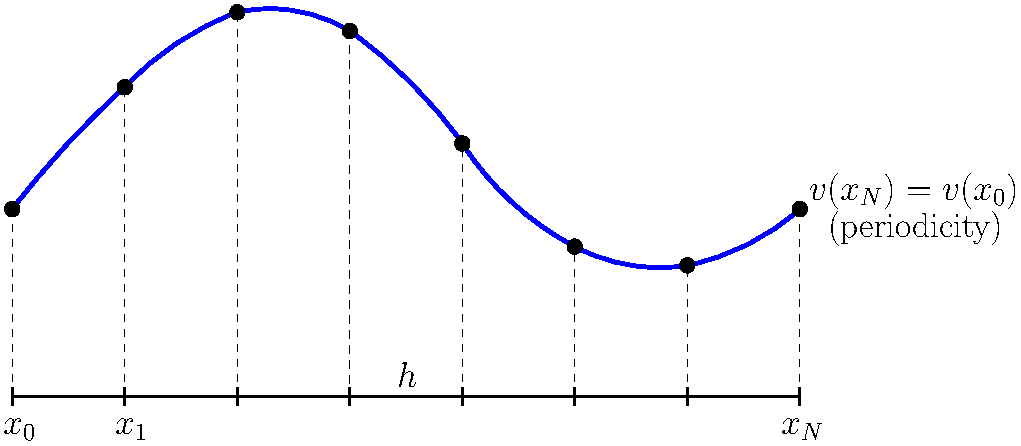
\includegraphics[width=10cm]{PeriodicFunction}
\end{figure}

Consider the vectors $\bm \varphi_k$, where
\begin{equation*}
  (\bm \varphi_k)_j = \text{e}^{\text{i} k x_j}, \qquad j,k=0,1,\ldots,N-1.
\end{equation*}

Note that the vector elements in $\bm \varphi_k$ represent the values of the
function $\varphi_k(x) = \text{e}^{\text{i}kx}$ sampled at the discrete points
$x_j, \quad j=0,1,\ldots,N-1$. Note also that the function $\varphi_k(x) =
\text{e}^{\text{i}kx}$ is an eigenfunction of the Laplace operator with periodic
boundary conditions.

The vectors $\{ \bm \varphi_k \}_{k=0}^{N-1}$ form a basis for the
$N$-dimensional vector space $\mathbb{C}^N$. In particular, we have that
\begin{equation*}
  \bm \varphi_k^\mathsf{H} \bm \varphi_l = N\delta_{kl},
  \qquad \qquad k,l=0,1,\ldots,N-1.
\end{equation*}

The vector
\begin{equation*}
  \bm v =
  \begin{pmatrix}
    v_0 & \cdots & v_{N-1}
  \end{pmatrix}^\intercal
  \in \mathbb{R}^N
\end{equation*}
can be expressed in this basis as
\begin{equation*}
  \bm v = \sum_{k=0}^{N-1} \hat{v}_k \bm \varphi_k \qquad \Rightarrow \qquad
  v_j = \sum_{k=0}^{N-1} \hat{v}_k (\bm \varphi_k)_j
        = \sum_{k=0}^{N-1} \hat{v}_k \text{e}^{\text{i} k x_j},
\end{equation*}
where $\hat{v}_k$, are the discrete Fourier coefficients given by
\begin{equation*}
  \hat{v}_k = \frac{1}{N} \sum_{j=0}^{N-1} v_j \text{e}^{-\text{i}k x_j}, \qquad \qquad
  \begin{matrix}
    x_j = j h \\
    h = 2\pi / N
  \end{matrix}
  \qquad k=0,1,\ldots,N-1
\end{equation*}

\subsubsection{Discrete Sine Transform (DST)}

The Discrete Sine Transform is applicable to a function $v(x)$ which is
\emph{periodic} with period $2 \pi$ and \emph{odd}. Discretize the function on
an equidistant grid on $[0,\pi]$ with $h=\pi/n$. Set
\begin{equation*}
  v_j = v(x_j) = v(jh) = v \left(\frac{j \pi}{n} \right), \qquad \qquad j=0,1,\ldots,n.
\end{equation*}

Since $v$ is odd,
\begin{equation*}
  v(x_0) = v(x_n) = 0.
\end{equation*}

The discretized function is therefore represented by the $(n-1)$ real values
$v_1,\ldots,v_{n-1}$, i.e. by the vector
\begin{equation*}
  \bm v = \begin{pmatrix} v_1 & \vdots & v_{n-1} \end{pmatrix}^\intercal
  \in \mathbb{R}^{n-1}.
\end{equation*}

An orthogonal basis for $\mathbb{R}^{n-1}$ is given by the vectors
$\bm \psi_k$, $k=1,\ldots,n-1$, where
\begin{align*}
  (\bm \psi_k)_j &= \sin \left( \frac{k j \pi}{n} \right), \qquad j=1,\ldots,n-1,
\end{align*}
and with
\begin{align*}
  \bm \psi_k^\intercal \bm \psi_l &=
  \begin{cases}
    \frac{n}{2}, & k=l, \\
    0, & k \not= 0.
  \end{cases}
\end{align*}

In terms of this basis, we can write $\bm v$ as
\begin{align*}
  v_j
  &= \sum_{k=1}^{n-1} \tilde{v}_k \sin \left( \frac{k j \pi}{n} \right), &\qquad j&=1,\ldots,n-1,
\end{align*}
where
\begin{align*}{2}
  \tilde{v}_k
  &= \frac{2}{n} \sum_{j=1}^{n-1} v_j \sin \left( \frac{j k \pi}{n} \right), &\qquad  k&=1,\ldots,n-1.
\end{align*}

We can also write this as $\tilde{\bm v} = \bm S \bm v$ (DST) and $\bm v = \bm
S^{-1} \tilde{\bm v}$ (inverse DST). Note that $\bm S$ and $\bm S^{-1}$ are
related as
\begin{equation*}
  \bm S = \frac{2}{n} \bm S^{-1}
\end{equation*}

Also note that
\begin{align*}
  \matQ = \sqrt{\frac{2}{n}} \bm S^{-1} = \sqrt{\frac{n}{2}} \bm S.
\end{align*}

Now, consider the matrix $\bff^{(N)}$ where
\begin{equation*}
  \begin{split}
    F_{k,j}^{(N)} &= \text{e}^{-\text{i}jkh} \\
    &= \cos \left( \frac{j k 2 \pi}{N} \right) -
    i \sin \left( \frac{j k 2 \pi}{N} \right),
    \qquad 0 \leq j,k \leq N-1.
  \end{split}
\end{equation*}

Note that
\begin{equation*}
  F_{k,j}^{(2 n)} = \cos \left( \frac{j k \pi}{n} \right)
  - i \sin \left( \frac{j k \pi}{n} \right), \qquad 0 \leq j,k \leq 2n-1.
\end{equation*}

Now, consider
\begin{align*}
  \bm v &= \begin{pmatrix} v_1 & \cdots & v_{n-1} \end{pmatrix}^\intercal \in \mathbb{R}^{n-1}.
\end{align*}
Construct the extended vector as an ``odd'' extension
\begin{align*}
  \bm w &= \begin{pmatrix} 0 & v_1 & \cdots & v_{n-1} & 0 & -v_{n-1} & \cdots & -v_1 \end{pmatrix}^\intercal
  \in \mathbb{R}^{2n}.
\end{align*}

First, note that
\begin{equation*}
  (\bff^{(2n)} \bm w)_k
  = \sum_{j=0}^{2n-1} \text{e}^{\frac{-\text{i}jk \pi}{n}} w_j
  = 2n \hat{w}_k,
\end{equation*}
where $\hat{w}$, $\quad k=0,1,\ldots,2n-1$ are the discrete Fourier coefficients. Second,
\begin{align*}
  (\bff^{(2n)} \bm w)_k
  &= \sum_{j=0}^{2n-1} \left[
    \cos \left( \frac{j k \pi}{n} \right)
    - i \sin \left( \frac{jk \pi}{n} \right)
    \right] w_j \\
  &= \sum_{j=0}^{2n-1} w_j \cos \left( \frac{jk \pi}{n} \right)
    - i \sum_{j=0}^{2n-1} w_j \sin \left( \frac{j k \pi}{n} \right) \\
  &= -2i \sum_{j=0}^{n-1} w_j \sin \left( \frac{j k \pi}{n} \right) \\
  &= -2i \sum_{j=1}^{n-1} w_j \sin \left( \frac{j k \pi}{n} \right) \qquad (\text{since } w_0=0),
\end{align*}
where the first sum vanishes because it is a product of an odd and an even sequence.

Hence
\begin{equation*}
  \frac{i}{2} ( \bff^{(2n)} \bm w)_k =
  \sum_{j=1}^{n-1} w_j \sin \left( \frac{j k \pi}{n} \right) = \frac{n}{2} \tilde{w}_k.
\end{equation*}

Since
\begin{equation*}
  w_j=v_j, \qquad j=1,\ldots,n-1,
\end{equation*}
it follows that
\begin{equation*}
  \widetilde{w}_k = \widetilde{v}_k, \qquad k=1,\ldots,n-1.
\end{equation*}

In summary, for $k=1,\ldots,n-1$,
\begin{align*}
  \tilde{v}_k = \tilde{w}_k
  &= \frac{2}{n} \cdot \frac{\text{i}}{2} (\bff^{(2n)} \bm w)_k \\
  &= \frac{\text{i}}{n} (\bff^{(2n)} \bm w)_k \\
  &= \frac{\text{i}}{n} 2n \hat{w}_k \\
  &= 2\text{i} \hat{w}_k.
\end{align*}

By computing the discrete Fourier coefficients $\hat{w}_k$, we can find the
discrete sine coefficients $\widetilde{v}_k$, $k=1,\ldots,n-1,$ where
\begin{equation*}
  \tilde{\bm v} = \bm S \bm v = \sqrt{\frac{2}{n}} \matQ \bm v.
\end{equation*}

The operator $(\bff^{(2n)} \bm w)$ can be computed efficiently by a FFT in
$\mathcal{O}(2n \log 2n) \sim \mathcal{O} (n \log n)$ operations.

This leads to the \emph{modified algorithm} for Poisson:
\begin{enumerate}
\item Compute $\tilde{\bm G}^\intercal$ in $\mathcal{O}(n^2\log n)$.
  \begin{align*}
    \tilde{\bm G} &= \matQ^\intercal \bm G \matQ \\
    \Rightarrow \quad \tilde{\bm G}^\intercal &= \matQ^\intercal \bm G^\intercal \matQ\\
                  &= \matQ \bm G^\intercal \matQ^\intercal \qquad (\matQ = \matQ^\intercal) \\
                  &= \matQ (\matQ \bm G)^\intercal \\
                  &= \sqrt{\frac{2}{n}}\bm S^{-1} \sqrt{\frac{n}{2}} (\bm S \bm G)^\intercal \\
                  &= \bm S^{-1} (\bm S \bm G)^\intercal
  \end{align*}
\item Compute $\tilde{\uu}^\intercal$ in $\mathcal{O}(n^2)$.
  \begin{align*}
    \tilde{U}_{ji} = \frac{\tilde{G}_{ji}}{\lambda_j + \lambda_i}
  \end{align*}
\item Compute $\uu$ in $\mathcal{O}(n^2\log n)$.
  \begin{align*}
    \uu &= \matQ \tilde{\uu} \matQ^\intercal \\
          &= \matQ (\matQ \tilde{\uu}^\intercal)^\intercal \\
          &= \bm S^{-1} (\bm S \tilde{\uu}^\intercal)^\intercal
  \end{align*}
\end{enumerate}

Again, recall that
\begin{equation*}
  \bm S = \frac{2}{n}\bm S^{-1}
\end{equation*}
and $\tilde{\bm v} = \bm S \bm v$ is obtained as
\begin{enumerate}
\item $\bm v \in \mathbb{R}^{n-1} \quad \rightarrow \quad \bm w \in \mathbb{R}^{2n}$
\item Compute $\hat{\bm w}$ via FFT in $\mathcal{O}(n \log n)$.
\item $\tilde{v}_k = 2\text{i} \hat{w}_k, \qquad k=1,\ldots,n-1.$
\end{enumerate}

\subsubsection{Numerical results}

A diagonalization solver based on the FFT. The code was run on a PC, Pentium III
with 512 MB RAM.

We define $\tau(n)$ as the total simulation time (in seconds) and $\tau_1(n) =
\tau(n)/n^2$ as the time spent per degree of freedom.

\begin{table}[h]
  \caption{
    Simulation results for the numerical approximation of the two-dimensional
    Poisson equation by the use of fast diagonalization techniques.
  }
  \label{tbl:numres-fft}
  \begin{center}
    \bgroup\def\arraystretch{1.2}
    \begin{tabular}{r|lll}
      \hline
      $n$ & $\tau(n)$ & $\tau_1(n)$ & $\tau_1(n) (m \times m)$ \\
      \hhline{====}
      $32$ & $2.36 \cdot 10^{-2}$ & $2.31 \cdot 10^{-5}$ & $1.76 \cdot 10^{-5}$ \\
      $64$ & $1.11 \cdot 10^{-1}$ & $2.71 \cdot 10^{-5}$ & $3.66 \cdot 10^{-5}$ \\
      $128$ & $5.19 \cdot 10^{-1}$ & $3.17 \cdot 10^{-5}$ & $7.34 \cdot 10^{-5}$ \\
      $256$ & $2.35$ & $3.58 \cdot 10^{-5}$ & $1.50 \cdot 10^{-4}$ \\
      $512$ & $10.5$ & $3.99 \cdot 10^{-5}$ & $3.96 \cdot 10^{-4}$ \\
      $1024$ & $46.2$ & $4.41 \cdot 10^{-5}$ & $8.33 \cdot 10^{-4}$ \\
      \hline
      & $\sim \mathcal{O}(n^2 \log n)$ & $\sim \mathcal{O}(\log n)$ & $\sim \mathcal{O}(n) $ \\
      \hline
    \end{tabular}
    \egroup
  \end{center}

\end{table}

See \autoref{tbl:numres-fft}. The source code follows.

\begin{lstlisting}[style=fortran]
  program poisson

  ! FORTRAN-program to solve the two-dimensional Poisson equation
  ! on a unit square using finite differences (five-point stencil),
  ! one-dimensional eigenvalue decompositions and fast sine transforms.
  ! In this example, the right hand side f=1.

  ! note: n needs to be a power of 2

  ! Einar M. Ronquist
  ! NTNU, October 2000

  parameter (n  = 256)
  parameter (m  = n-1)
  parameter (nn = 4*n)

  real*8    diag(m), b(m,m), bt(m,m)
  real*8    pi
  real*8    z(0:nn-1)
  real*4    tarray(2), t1, t2, dt

  h    = 1./n
  pi   = 4.*datan(1.)

  do i=1,m
    diag(i) = 2*(1-dcos(i*pi/n))
  enddo

  do j=1,m
    do i=1,m
      b(i,j) = h*h
    enddo
  enddo

  do j=1,m
    call fst (b(1,j), n, z, nn)
  enddo
  call transp (bt, b, m)
  do i=1,m
    call fstinv (bt(1,i), n, z, nn)
  enddo

  do j=1,m
    do i=1,m
      bt(i,j) = bt(i,j)/(diag(i)+diag(j))
    enddo
  enddo

  do i=1,m
    call fst (bt(1,i), n, z, nn)
  enddo
  call transp (b, bt, m)
  do j=1,m
    call fstinv (b(1,j), n, z, nn)
  enddo

  umax = 0.0
  do j=1,m
    do i=1,m
      if (b(i,j) .gt. umax) umax = b(i,j)
    enddo
  enddo

  write(6,*) ' '
  write(6,*) umax

  stop
  end

  subroutine transp (at, a, m)

  ! set at equal to the transpose of a

  real*8 a(m,m), at(m,m)

  do j=1,m
    do i=1,m
      at(j,i) = a(i,j)
    enddo
  enddo

  return
  end
\end{lstlisting}


%-------------------------------------------------------------------------------
\newpage
\input{09-finite-element-method}

%-------------------------------------------------------------------------------
\newpage

\newcommand{\xC}{\mathbb{C}}
\newcommand{\xR}{\mathbb{R}}
\newcommand{\xRd}{{\xR^d}}
\newcommand{\xRN}{{\xR^N}}
\newcommand{\xMNR}{{M_N(\xR)}}
\newcommand{\bb}{{\boldsymbol b}}
\newcommand{\ee}{{\boldsymbol e}}
\newcommand{\ev}{{\boldsymbol \epsilon}}
\newcommand{\rr}{{\boldsymbol r}}
\newcommand{\xx}{{\boldsymbol x}}
\newcommand{\hx}{\hat{\boldsymbol x}}
\newcommand{\yy}{{\boldsymbol y}}
\newcommand{\ww}{{\boldsymbol w}}
\newcommand{\zz}{{\boldsymbol z}}
\newcommand{\mA}{{\mathrm A}}
\newcommand{\mB}{{\mathrm B}}
\newcommand{\mC}{{\mathrm C}}
\newcommand{\mD}{{\mathrm D}}
\newcommand{\mG}{{\mathrm G}}
\newcommand{\mH}{{\mathrm H}}
\newcommand{\mJ}{{\mathrm J}}
\newcommand{\mL}{{\mathrm L}}
\newcommand{\mLs}{{\mathrm L_0}}
\newcommand{\mM}{{\mathrm M}}
\newcommand{\mRs}{{\mathrm R_0}}
\newcommand{\mR}{{\mathrm R}}
\newcommand{\mP}{{\mathrm P}}
\newcommand{\mQ}{{\mathrm Q}}
\newcommand{\mU}{{\mathrm U}}
\newcommand{\mId}{{\mathbf{Id}}}
\newcommand{\mII}{{\mathbf{\mathbb{I}}}}
\newcommand{\Seq}[1]{\bigl(#1\bigr)}
\newcommand{\Cond}[1]{\mathcal{C}(#1)}
\newcommand{\Order}[1]{\mathcal{O}\left(#1\right)}
\newcommand{\norm}[1]{{\lVert #1 \rVert}}
\newcommand{\norminf}[1]{\norm{#1}_{\infty}}

\newcommand{\InnerK}[2]{{{\mathbf\langle}\;#1\:,\: #2 \;{\rangle}}}
\newcommand{\Inner}[2]{{{\scriptstyle\mathbf{(}}\;#1\:,\: #2 \;{\scriptstyle\mathbf{)}}}}

\newcommand{\argmin}[1]{\mathop{\underset{#1}{\mathrm{argmin}}}\:}

\chapter{Linear Solvers}

\section{Direct methods}

\section{Iterative methods}

As seen in the previous lecture, direct methods can theoretically compute exact solutions $\xx\xRN$ to linear systems in the form of:
\[
\mA \xx = \bb
\]
with matrix with real coefficients $\mA\in\xMNR$ and given data $\bb\in\xRN$, in a determined finite number of steps.

As computing the inverse of the matrix is unrealistic, several methods were introduced based on factorizations of the type $\mA = \mP\;\mQ$ where $\mP$ and $\mQ$ have a structure simplifying the resolution of the system: diagonal, banded, triangular.

Methods like $\mL\mU$, Cholevski take advantage of the existence of a decomposition involving triangular matrices while $\mQ\mR$ for example, involves the construcion of an orthogonal basis.
All methods prove to be quite expensive, hard to parallelize due to the sequential nature of the algorithm and prone to error propagation.

Iterative methods have been developed for:
\begin{itemize}
\item solving very large linear systems with direct methods is in practice not possible due to the complexity in term of computational operations and data,
\item taking advantage of sparse system for which the structure of the matrix can result in dramatic speed-up (this is the case for numerical schemes for PDEs),
\item using the fact that some systems like PDEs discretizations are already formulated in an iterative fashion.
\end{itemize}

\medskip
In this section, we discuss briefly the computational properties of iterative methods for solving linear systems.
Computing the exact solution is not a requirement anymore but instead the algorithm is supposed to converge asymptotically to the exact solution: the algorithm is stopped when the approximate solution is deemed \textit{close enough} to the exact solution in a sense to be defined.
A parameter used as stopping criterion triggers the completion of the algorithm.

\medskip
The general idea of these methods is to introduce a splitting of the form:
\[
\mA = \mG - \mH
\]
such the solution $\xx$ satisfies:
\[
\mG \xx = \bb + \mH \xx
\]

Similarly to fixed-point methods we can define a sequence of approximate solutions $\Seq{\xx^k}$ satisfying relations of the form:
\[
\mG \hx^{k+1} = \bb + \mH \hx^{k}
\]
with $\mG$ invertible.

The matrix viewed as a linear mapping in $\xRN$, the counterpart of such approaches is given by the Brouwer Theorem in finite dimension, where a continuous mapping $f : \Omega \rightarrow \Omega$ with $\Omega$ compact of $\xRN$ admits a fixed-point $\xx^\star$ satisfying $f(\xx^\star) = \xx^\star$ and is contracting.

\medskip
Methods introduced depend on the iteration defined by the splitting and call for several questions regarding the computational aspects:
\begin{enumerate}
\item How can the convergence be ensure?
\item How fast is the convergence?
\item How expensive is each iteration?
\item How does the algorithm behave with respect to numerical error?
\end{enumerate}

\medskip
The question of the convergence is addressed by proving an estimate on error vectors in terms of iteration error $\hat{\ev}^k = \hx^{k+1}-\hx^{k}$ or global error: $\ev^k = \hx^{k}-\xx$. The convergence rate $\alpha$ means that $C > 0$, $\lvert\ev^{k+1}\rvert \leq C \lvert\ev^{k}\rvert^\alpha$.

\medskip
For example, substituting $\hx^{k+1} = \mG^{-1}\bb + \mG^{-1}\mH \hx^{k}$ in $\hat{\ev}^k = \hx^{k+1}-\hx^{k}$ gives a relation between successive iteration errors:
\[
\hat{\ev}^{k} = \mG^{-1}\mH\;\hat{\ev}^{k-1}
\]
with $\mM = \mG^{-1}\mH$ the iteration matrix, and recursively $\hat{\ev}^{k} = (\mG^{-1}\mH)^{k+1}\hat{\ev}^{0}$.
Convergence is then conditioned to the existence of a contraction factor $K < 1$ such that $\norminf{\hat{\ev}^{k}} \leq K\;\norminf{\hat{\ev}^{k-1}}$ ensuring decrease of the error.

\medskip
In terms of the matrix $\mM$, this translate for the spectral radius $\rho(\mM)$ as $\rho(\mM) < 1$ since in that case $\lim_{k\rightarrow\infty} M^k \hat{\ev}^{0} = 0_{\xRN}$.
The smaller the spectral radius, the faster the convergence.

\medskip
Each method is described briefly and qualitatively with just the necessary ingredients to discuss practical implementations.

\section{Relaxation methods}

Consider the relations for each row $i=1,\dots,N$:
\begin{equation}
\xx_i = \frac{1}{a_{ii}}\Bigl( b_i - \sum_{i\neq j} a_{ij} \xx_j \Bigr)
\end{equation}

Let us introduce two methods based on constructing sequences of approximate solutions $\Seq{\hx^k}$, $k\geq1$ given an initial guess $\hx^0 \in \xRN$ and then associated relaxation methods.

\section{Jacobi, methods of simultaneous displacements}

\begin{equation}
\hx^{k+1}_i = \frac{1}{a_{ii}}\Bigl( b_i - \sum_{i\neq j} a_{ij} \hx^{k}_j \Bigr)
\end{equation}

\medskip
\textbf{Convergence:} the global error $\ev^k$ is controlled by
\begin{equation*}
\norm{\ev^{k+1}} \leq \sum_{i\neq j} \Bigl\lvert\frac{a_{ij}}{a_{ii}}\Bigr\rvert\;\norm{\ev^{k}} \leq K^k \; \norm{\ev^{1}}
\end{equation*}
It is then enough if the matrix is strictly diagonally dominant.
Expressing the iteration error gives directly that $\mM = \mG^{-1}\mH$ such that $\rho(\mM)< 1$.

\medskip
\textbf{Algorithm:} the splitting is
\[
\mA = \mD - \mH
\]
with $\mD = \mathrm{diag}(A)$, thus
\[
\hx^{k+1} = \mD^{-1}(\bb + \mH \hx^{k})
\]

\medskip
\textbf{Implementation:}
\begin{enumerate}
\item Parallelization component by component is possible since there is only dependency on $\hx^{k}$.
\item Memory requirement for storing both $\hx^{k+1}$ and $\hx^{k}$ at each iteration.
\end{enumerate}

\section{Gauss--Seidel, methods of sucessive displacements}

In Jacobi iterations, notice that sequential ordered computation of terms
\begin{equation}
\hx^{k+1}_i = \frac{1}{a_{ii}}\Bigl( b_i - \sum_{i\neq j} a_{ij} \hx^{k}_j \Bigr)
\end{equation}
involves components $\hx^{k}_j$ which are also computed for $\hx^{k+1}$ if $j < i$.
\begin{equation}
\hx^{k+1}_i = \frac{1}{a_{ii}}\Bigl( b_i - \sum_{i < j} a_{ij} \hx^{k+1}_j - \sum_{i > j} a_{ij} \hx^{k}_j \Bigr)
\end{equation}

\medskip
\textbf{Algorithm:} the splitting is
\[
\mA = \mL - \mRs
\]
with $\mL = \mD + \mLs$ lower-triangular matrix and $\mRs$ strict upper-triangular matrix, thus
\[
\hx^{k+1} = \mD^{-1}(\bb - \mLs \hx^{k+1} + \mRs \hx^{k})
\]
or
\[
\mL\;\hx^{k+1} = \mD^{-1}(\bb + \mRs \hx^{k})
\]
Recast under the usual form:
\[
\hx^{k+1} = \mL^{-1}(\bb + \mRs \hx^{k})
\]
and the iteration matrix is $\bar \mM = \mL^{-1}\mRs$.

\medskip
\textbf{Convergence:} the global error $\ev^k$ is controlled by
\begin{equation*}
\norm{\ev^{k+1}} \leq \frac{\displaystyle\sum_{i > j} \Bigl\lvert\frac{a_{ij}}{a_{ii}}\Bigr\rvert}{1 - \displaystyle\sum_{i < j} \Bigl\lvert\frac{a_{ij}}{a_{ii}}\Bigr\rvert}\;\norm{\ev^{k}} \leq \bar{K}^k \; \norm{\ev^{1}}
\end{equation*}
If the Jacobi contraction factor $K < 1$ then $\bar{K} < 1$.
Expressing the iteration error gives directly that $\bar\mM = \mL^{-1}\mRs$ such that $\rho(\bar\mM)< 1$.


\medskip
\textbf{Implementation:}
\begin{enumerate}
\item Parallelization component by component is not possible easily since there is serialization for each row $i$ due to the dependency on $\hx_j^{k+1}$, $j < i$.
\item Memory requirement is only for storing one vector of $\xRN$ at each iteration.
\end{enumerate}


\section{Relaxation of Jacobi and Gauss-Seidel}

Relaxation methods consists of adding a linear combination of the approximate solution at the previous iteration to minimize the spectral radius for convergence, using the relaxation parameter $\gamma \in (0,1)$.

\medskip
\begin{enumerate}
\item Jacobi Over-Relaxation (JOR):
\begin{equation}
\hx^{k+1}_i = (1 - \gamma)\;\hx^{k}_i + \gamma \frac{1}{a_{ii}}\Bigl( b_i - \sum_{i\neq j} a_{ij} \hx^{k}_j \Bigr)
\end{equation}
which reads in matricial form
\[
\hx^{k+1} = \mM_\gamma \hx^{k} + \gamma\mD^{-1}\;\bb
\]
with $\mM_\gamma = (1-\gamma)\mII + \gamma\mD^{-1} \mH$

\medskip
\item Successive Over-Relaxation (SOR):
\begin{equation}
\hx^{k+1}_i = (1-\gamma)\;\hx^{k}_i + \gamma \frac{1}{a_{ii}}\Bigl( b_i - \sum_{i < j} a_{ij} \hx^{k+1}_j - \sum_{i > j} a_{ij} \hx^{k}_j \Bigr)
\end{equation}
which reads in matricial form
\[
\hx^{k+1} = \mM_\gamma \hx^{k} + \gamma\mC\;\bb
\]
with $\mM_\gamma = (1 + \gamma\mD^{-1}\mLs^{-1} )^{-1} \bigl[(1-\gamma)\mII + \gamma\mD^{-1} \mRs \bigr]$ and $\mC = (1 + \gamma\mD^{-1}\mLs^{-1} )^{-1} \mD^{-1}$
\end{enumerate}

\medskip
The relaxation parameter $\gamma$ cannot be known \textit{a priori} and is usually determined by heuristics.

\section{Parallelization of Gauss--Seidel}

Overcoming the serialization in Gauss--Seidel is possible if the matrix is sparse.
Taking advantage of the fact that components does not all possess connectivities with each other: such dependencies can be built from the sparsity pattern then decoupled graphs identified:
\begin{enumerate}
\item Component Dependency-Graph: generate a graph to reorder entries such that dependencies are avoided.
\item Red--Black coloring: special case for two-dimensional problems.
\end{enumerate}



\section{Krylov-subspace methods}

The idea of these methods is that the solution is decomposed on a sequence of orthogonal subspaces.

If $\mA$ is symmetric definite positive it induces the corresponding scalar product:
\[
\InnerK{\xx}{\yy}_A = \Inner{\mA \xx}{\yy} = \yy^T\mA\xx
\]
with $\Inner{\mA \cdot}{\cdot}$ canonical scalar product in $\xRN$.
The vectors $(\ee_1, \dots, \ee_N)$ are said $\mA$-conjugate if $\ee_j^T\mA\ee_i = 0$ for $i\neq j$: they are orthogonal for the scalar-product induced by $\mA$.

\section{Principle of descent methods: Steepest Gradient }

Minimisation of the residual:
\begin{equation*}
\xx^\star = \argmin{\xx}\mJ(\xx) : \mJ(\xx) = \frac{1}{2}\InnerK{\xx}{\xx}_A - \Inner{\bb}{\xx}
\end{equation*}

Construct a sequence of solutions to approximate minimization problems, given $\hx^k$:
\[
\mJ(\hx^{k+1}) \leq \mJ(\hx^k)
\]
where $\hx^{k+1} = \hx^{k} + \alpha_{k+1} \ee^{k+1}$, with $\alpha_{k+1}$ a descent factor and $\ee_{k+1}$ a direction.

\medskip
For the Steepest Gradient:
\begin{enumerate}
\item take the direction given by $-\nabla\mJ(\hx^k) = \bb - \mA \hx^k$ which is the residual $\rr_k = \bb - \mA\hx^k$, thus $\hx^{k+1} = \hx^{k} + \alpha_{k+1} \rr_k$.
\item choose the descent factor $\alpha^{k+1}$ minimizing the functional $\mJ(\hx^{k} + \alpha_{k+1} \rr_k)$:
\[
\alpha_{k+1} = \frac{\rr_k^T\bb}{\rr_k^T\mA\rr_k}
\]
\end{enumerate}

\medskip
The speed of convergence is bounded by $\Order{1- \Cond{\mA}^{-1}}$ with $\Cond{\mA}$ the condition number of $\mA$.
The gradient direction may not be optimal, Conjugate Gradient methods improve the choice of $\Seq{\ee_k}$.

\section{Conjugate Gradient}

The Conjugate Gradient (CG) is a Krylov-subspace algorithm for symmetric positive definite matrices.

\medskip
Given $\hx^0$, $\Seq{\hx^k}$ is a sequence of solutions to approximate $k$-dimensional minimisation problems.

\medskip
For the Conjugate Gradient:
\begin{enumerate}
\item take the direction $\ee_{k+1}$ such that $\bigl(\ee_1, \dots, \ee_{k}, \ee_{k+1}\bigr)$ is $A$-conjugate, thus $\hx^{k+1} = \hx^{k} + \alpha_{k+1} \ee_{k+1}$.
\item choose the descent factor $\alpha^{k+1}$ minimizing the functional $\mJ(\hx^{k} + \alpha_{k+1} \ee_k)$, which is defined by
\[
\alpha_j = \frac{\ee^T_j\rr_{k-1}}{\ee^T_j\mA\ee_j}
\]
and with $\ee^T_j\rr_{k-1} \neq 0$ (unless the exact solution is reached).
\end{enumerate}

\medskip
The construction of $\bigl(\ee_1, \dots, \ee_{k+1}\bigr)$ is done by orthogonalization of residuals by Gram--Schmidt:
\[
\ee_{k+1} = \rr_k - \frac{\ee^T_k\mA\rr_{k-1}}{\ee^T_k\mA\ee_k}\ee_k
\]
so that $\rr_{k+1} = \bb - \mA\hx^{k+1} = \rr^k - \alpha_{k+1}\mA\ee_{k+1}$

\medskip
After $N$ steps, the $A$-conjugate basis of $\xRN$ is done and the exact solution is reached:
\[
 \xx = \sum_{j=1}^N \alpha_j \ee_j
\]

\medskip
For any $k$, the speed of convergence is bounded by
\[
\Order{ \frac{ 1-\sqrt{\Cond{\mA}} } { 1+\sqrt{\Cond{\mA}} } }^{2k}
\]
in the norm induced by $A$, with $\Cond{\mA}$ the conditioning of $\mA$.

\medskip
The Conjugate Gradient can therefore be seen as a direct methods but in practice:
\begin{itemize}
\item the iterative computation of the $A$-conjugate basis suffers from the same issue of numerical error propagation as the $\mQ\mR$ factorization leading to a loss of orthogonality,
\item the convergence is slow, which makes it unrealistic to compute the exact solution for large systems,
\end{itemize}
so it is used as an iterative method.

\medskip
Example algorithm on first steps:
\begin{enumerate}
\item Given $\hx^0 = 0$, set $\rr_0 = \bb - \mA \hx^0$ and $\ee_1 = \rr_0$,
\item Take $\hx_1 = \alpha_1 \ee_1$, then $\alpha_1\ee_1^T \mA \ee_1 = \ee_1^T \bb$, thus
\[
\alpha_1 = \frac{\rr^T_0\bb}{\rr^T_0\mA\rr_0}
\]
\item Compute the residual:
\[
\rr_1 = \bb - \mA \hx^1
\]
\item Compute the direction:
\[
\ee_{2} = \rr_1 - \frac{\ee^T_1\mA\rr_{0}}{\ee^T_1\mA\ee_1}\ee_1
\]
\item Compute the factor:
\[
\alpha_2 = \frac{\ee^T_2\bb}{\ee^T_2\mA\ee_2}
\]
\item Update the solution:
\[
\hx^2 = \hx^1 + \alpha_2 \ee_2
\]
\item \dots
\end{enumerate}

\medskip
The algorithm iteration reads:
\begin{enumerate}
\item Compute the residual:
\[
\rr_k = \bb - \mA \hx^{k}
\]
\item Compute the direction:
\[
\ee_{k+1} = \rr_k - \frac{\ee^T_{k}\mA\rr_{k-1}}{\ee^T_k\mA\ee_k}
\]
\item Compute the factor:
\[
\alpha_{k+1} = \frac{\ee^T_{k+1}\bb}{\ee^T_{k+1}\mA\ee_{k+1}}
\]
\item Update the solution:
\[
\hx^{k+1} = \hx^k + \alpha_{k+1} \ee_{k+1}
\]\end{enumerate}
which requires two matrix-vector multiplications per loop, $\mA\hx^{k}$ then $\mA\ee_{k+1}$
Using $\rr_{k+1} = \rr^k - \alpha_{k+1}\mA\ee_{k+1}$ saves one matrix-vector multiplication.


\medskip
While the residual norm $\varrho_k = \norm{\rr_k}^2_2$ is big:
\begin{enumerate}
\item Compute the projection:
\[
\beta_k = \frac{\varrho_k}{\varrho_{k-1}}
\]
\item Compute the direction:
\[
\ee_{k+1} = \rr_k + \beta_k\ee_k
\]
\item Compute the factor:
\[
\ww = \mA\ee_{k+1};\quad \alpha_{k+1} = \frac{\varrho_k}{\ee^T_{k+1}\ww}
\]
\item Update the solution:
\[
\hx^{k+1} = \hx^k + \alpha_{k+1} \ee_{k+1}
\]
\item Update the residual:
\[
\rr^{k+1} = \rr^k - \alpha_{k+1} \ww
\]
\end{enumerate}

\section{Preconditioners}

While seeing the Conjugate Gradient as a pure iterative method relieves from concerns regarding orthogonality loss, the convergence is still slow as soon as the condition number of the matrix is bad.

\medskip
Preconditioning the system consists in finding a non-singular symmetric matrix $\mC$ such that $\tilde \mA = \mC^{-1}\mA\mC^{-1}$ and the conjugate gradient is applied to
\[
\tilde\mA \tilde\xx = \tilde\bb
\]
with $\tilde\xx = \mC^{-1}\xx$ and $\tilde\bb = \mC^{-1}\bb$.

\medskip
With:
\begin{itemize}
\item $\mM = \mC^2$
\item $\ee_k = \mC^{-1}\tilde\ee_k$
\item $\hx_k = \mC^{-1}\tilde\hx_k$
\item $\zz_k = \mC^{-1}\tilde\rr_k$
\item $\rr_k = \mC\tilde\rr_k = \bb - \mA\hx_k$
\end{itemize}
and $\mM$ is a symmetric positive definite matrix called the preconditioner.

\medskip
While the residual norm $\varrho_k = \norm{\rr_k}^2_2$ is big:
\begin{enumerate}

\item Solve:
\[
\mM\zz_{k} = \rr_k
\]
\item Compute the projection:
\[
\beta_k = \frac{\zz_{k}^T\rr_k}{\zz_{k-1}^T\rr_{k-1}}
\]
\item Compute the direction:
\[
\ee_{k+1} = \zz_k + \beta_k\ee_k
\]
\item Compute the factor:
\[
\alpha_{k+1} = \frac{\zz_{k}^T\rr_k}{\ee^T_{k+1}\mA\ee_{k+1}}
\]
\item Update the solution:
\[
\hx^{k+1} = \hx^k + \alpha_{k+1} \ee_{k+1}
\]
\item Update the residual:
\[
\rr^{k+1} = \rr^k - \alpha_{k+1} \ww
\]
\end{enumerate}

\medskip
The linear system $\mM\zz_{k} = \rr_k$ should be easy to solve and can lead to fast convergence, typically $\Order(\sqrt{N})$.
Since
\[
\mM\zz_{k} = \bb - \mA\hx_k
\]
Then an iterative relation appears:
\[
\hx_{k+1} = \mM^{-1}\bigl(\bb - \mA\hx_k\bigr)
\]
therefore iterative methods like Jacobi, Gauss-Seidel and relaxation methods can be used.

\section{Power method}

This method is used for finding the dominant eigenvalues of a matrix $\mA \in \xMNR$ of $N$ eigenvectors $\Seq{\vv_i}$ with associated eigenvalues $\Seq{\lambda_i}$ ordered in decreasing module.
The eigenvalues are either real or conjugate complex pairs.

\medskip
Given a random vector $\xx^0$, construct a sequence of vectors $\Seq{\hx^k}$ such that
\[
\hx^{k+1} = \mA \hx^k
\]
then $\forall k \geq 0$
\[
\hx^k = \sum_{i=0}^{N-1} \lambda_i^k \xi_i \vv_i
\]
for some coefficients $\Seq{\vv_i}$.

\medskip
Assume that $\lambda_0$ is a dominant real eigenvalue and $\xi_0 \neq 0$, then
\[
\hx^k = \lambda_0^k \bigl(\xi_0 \vv_0 + \rr_k \bigr)
\]
with the residual $\rr_k$ defined as
\[
\rr_k = \lambda_0^{-k} \sum_{i=1}^{N-1} \lambda_i^k \xi_i \vv_i
\]
and $\lim_{k\rightarrow\infty} \rr_k = O_{\xRN}$.
To the limit $\hx_{k+1} \approx \lambda_0 \hx^k \approx \lambda_0\xi_0\vv0$ almost parallel to the first eigenvector.

\medskip
\begin{itemize}
\item This method is fast to compute the spectral radius for the Jacobi method and relaxation parameters.
\item The convergence is geometric and the speed depends on the ratio $\lvert \lambda_1 / \lambda_0\rvert$.
\item If the matrix is symmetric, the convergence speed can be doubled.
\item If $\lambda_0$ is very large or very small then taking high powers lead to numerical issues, the algorithm requires a normalization.
\end{itemize}


%-------------------------------------------------------------------------------
\newpage
\input{11-parallel-io}

%===============================================================================
\newpage
\bibliography{main}

\end{document}

